\documentclass[a4paper]{article}

\def\npart {IA}
\def\nterm {Lent}
\def\nyear {2015}
\def\nlecturer {G.\ I.\ Ogilvie}
\def\ncourse {Dynamics and Relativity}

\input{header}

\begin{document}
\maketitle
{\small
\noindent\emph{Familiarity with the topics covered in the non-examinable Mechanics course is assumed.}
\vspace{10pt}

\noindent\textbf{Basic concepts}\\
Space and time, frames of reference, Galilean transformations. Newton's laws. Dimensional analysis. Examples of forces, including gravity, friction and Lorentz.\hspace*{\fill} [4]

\vspace{10pt}
\noindent\textbf{Newtonian dynamics of a single particle}\\
Equation of motion in Cartesian and plane polar coordinates. Work, conservative forces and potential energy, motion and the shape of the potential energy function; stable equilibria and small oscillations; effect of damping.

\vspace{5pt}
\noindent Angular velocity, angular momentum, torque.

\vspace{5pt}
\noindent Orbits: the $u(\theta)$ equation; escape velocity; Kepler's laws; stability of orbits; motion in a repulsive potential (Rutherford scattering). Rotating frames: centrifugal and coriolis forces. *Brief discussion of Foucault pendulum.*\hspace*{\fill} [8]

\vspace{10pt}
\noindent\textbf{Newtonian dynamics of systems of particles}\\
Momentum, angular momentum, energy. Motion relative to the centre of mass; the two body problem. Variable mass problems; the rocket equation.\hspace*{\fill} [2]

\vspace{10pt}
\noindent\textbf{Rigid bodies}\\
Moments of inertia, angular momentum and energy of a rigid body. Parallel axes theorem. Simple examples of motion involving both rotation and translation (e.g.\ rolling).\hspace*{\fill} [3]

\vspace{10pt}
\noindent\textbf{Special relativity}\\
The principle of relativity. Relativity and simultaneity. The invariant interval. Lorentz transformations in $(1 + 1)$-dimensional spacetime. Time dilation and length contraction. The Minkowski metric for $(1 + 1)$-dimensional spacetime. Lorentz transformations in $(3 + 1)$ dimensions. 4-vectors and Lorentz invariants. Proper time. 4-velocity and 4-momentum. Conservation of 4-momentum in particle decay. Collisions. The Newtonian limit.\hspace*{\fill} [7]}

\tableofcontents
\setcounter{section}{-1}
\section{Introduction}
You've been lied to. You thought you applied for mathematics. And here you have a course on physics. No, this course is not created for students taking the ``Maths with Physics'' option. They don't have to take this course (don't ask why).

Ever since Newton invented calculus, mathematics is becoming more and more important in physics. Physicists seek to describe the universe in a few equations, and derive everyday (physical) phenomena as mathematical consequences of these equations.

In this course, we will start with Newton's laws of motion and use it to derive a lot of physical phenomena, including planetary orbits, centrifugal forces\footnote{Yes, they exist.} and the motion of rotating bodies.

The important thing to note is that we can ``prove'' all these phenomena just under the assumption that Newton's laws are correct (plus the formulas for, say, the strength of the gravitational force). We are just doing mathematics here. We don't need to do any experiments to obtain the results (of course, we need experiments to verify that Newton's laws are indeed the equations that describe this universe).

However, it turns out that Newton was wrong. While his theories were accurate for most everyday phenomena, they weren't able to adequately describe electromagnetism. This lead to Einstein discovering \emph{special relativity}. Special relativity is also required to describe motion that is very fast. We will have a brief introduction to special relativity at the end of the course.

\section{Newtonian dynamics of particles}
Newton's equations describe the motion of a \emph{(point) particle}.
\begin{defi}[Particle]
  A \emph{particle} is an object of insignificant size, hence it can be regarded as a point. It has a \emph{mass} $m > 0$, and an \emph{electric charge} $q$.

  Its position at time $t$ is described by its \emph{position vector}, $\mathbf{r}(t)$ or $\mathbf{x}(t)$ with respect to an origin $O$.
\end{defi}
Depending on context, different things can be considered as particles. We could consider an electron to be a point particle, even though it is more accurately described by the laws of quantum mechanics than those of Newtonian mechanics. If we are studying the orbit of planets, we can consider the Sun and the Earth to be particles.

An important property of a particle is that it has no \emph{internal structure}. It can be completely described by its position, momentum, mass and electric charge. For example, if we model the Earth as a particle, we will have to ignore its own rotation, temperature etc.

If we want to actually describe a rotating object, we usually consider it as a collection of point particles connected together, and apply Newton's law to the individual particles.

As mentioned above, the position of a particle is described by a position \emph{vector}. This requires us to pick an origin of the coordinate system, as well as an orientation of the axes. Each choice is known as a frame of reference.

\begin{defi}[Frame of reference]
  A \emph{frame of reference} is a choice of coordinate axes for $\mathbf{r}$.
\end{defi}
We don't impose many restrictions on the choice of coordinate axes. They can be fixed, moving, rotating, or even accelerating.

Using the position vector $\mathbf{r}$, we can define various interesting quantities which describe the particle.
\begin{defi}[Velocity]
  The \emph{velocity} of the particle is
  \[
    \mathbf{v} = \dot{\mathbf{r}} = \frac{\d \mathbf{r}}{\d t}.
  \]
\end{defi}

\begin{defi}[Acceleration]
  The \emph{acceleration} of the particle is
  \[
    \mathbf{a} = \dot{\mathbf{v}} = \ddot{\mathbf{r}} = \frac{\d^2 \mathbf{r}}{d t^2}.
  \]
\end{defi}

\begin{defi}[Momentum]
  The \emph{momentum} of a particle is
  \[
    \mathbf{p} = m\mathbf{v} = m\dot{\mathbf{r}}.
  \]
  $m$ is the \emph{inertial mass} of the particle, and measures its reluctance to accelerate, as described by Newton's second law.
\end{defi}

\subsection{Newton's laws of motion}
We will first state Newton's three laws of motion, and then discuss them individually.
\begin{law}[Newton's First Law of Motion]
  A body remains at rest, or moves uniformly in a straight line, unless acted on by a force. (This is in fact Galileo's Law of Inertia)
\end{law}

\begin{law}[Newton's Second Law of Motion]
   The rate of change of momentum of a body is equal to the force acting on it (in both magnitude and direction).
\end{law}

\begin{law}[Newton's Third Law of Motion]
  To every action there is an equal and opposite reaction: the forces of two bodies on each other are equal and in opposite directions.
\end{law}
The first law might seem redundant given the second if interpreted literally. According to the second law, if there is no force, then the momentum doesn't change. Hence the body remains at rest or moves uniformly in a straight line.

So why do we have the first law? Historically, it might be there to explicitly counter Aristotle's idea that objects naturally slow down to rest. However, some (modern) physicists give it an alternative interpretation:

Note that the first law isn't always true. Take yourself as a frame of reference. When you move around your room, things will seem like they are moving around (relative to you). When you sit down, they stop moving. However, in reality, they've always been sitting there still. On second thought, this is because you, the frame of reference, is accelerating, not the objects. The first law only holds in frames that are themselves not accelerating. We call these \emph{inertial frames}.
\begin{defi}[Inertial frames]
  \emph{Inertial frames} are frames of references in which the frames themselves are not accelerating. Newton's Laws only hold in inertial frames.
\end{defi}
Then we can take the first law to assert that inertial frames exists. Even though the Earth itself is rotating and orbiting the sun, for most purposes, any fixed place on the Earth counts as an inertial frame.

\subsection{Galilean transformations}
The goal of this section is to investigate inertial frames. We know that inertial frames are not unique. Given an inertial frame, what other inertial frames can we obtain?

First of all, we can rotate our axes or move our origin. In particular, we can perform the following operations:
\begin{itemize}
  \item Translations of space:
    \[
      \mathbf{r}' = \mathbf{r} - \mathbf{r}_0
    \]
  \item Translations of time:
    \[
      t' = t - t_0
    \]
  \item Rotation (and reflection):
    \[
      \mathbf{r}' = R\mathbf{r}
    \]
    with $R\in \Or(3)$.
\end{itemize}
These are not very interesting. They are simply symmetries of space itself.

The last possible transformation is \emph{uniform motion}. Suppose that $S$ is an inertial frame. Then any other frame $S'$ in uniform motion relative to $S$ is also inertial:
\begin{center}
  \begin{tikzpicture}
    \node at (0, 1.5) [left] {$S$};
    \node at (4, 1.5) [left] {$S'$};
    \draw [->] (0, 0) -- (0, 3) node [above] {$y$};
    \draw [->] (0, 0) -- (3, 0) node [right] {$x$};
    \draw [->] (4, 0) -- (4, 3) node [above] {$y'$};
    \draw [->] (4, 0) -- (7, 0) node [right] {$x'$};
    \draw [->] (4, 1.5) -- (4.5, 1.5) node [right] {$\mathbf{v}$};
  \end{tikzpicture}
\end{center}
Assuming the frames coincide at $t = 0$, then
\begin{align*}
  x' &= x - vt\\
  y' &= y\\
  z' &= z\\
  t' &= t
\end{align*}
Generally, the position vector transforms as
\[
  \mathbf{r}' = \mathbf{r} - \mathbf{v}t,
\]
where $\mathbf{v}$ is the (constant) velocity of $S'$ relative to $S$. The velocity and acceleration transform as follows:
\begin{align*}
  \dot{\mathbf{r}}' &= \dot{\mathbf{r}} - \mathbf{v}\\
  \ddot{\mathbf{r}}' &= \ddot{\mathbf{r}}
\end{align*}
\begin{defi}[Galilean boost]
  A \emph{Galilean boost} is a change in frame of reference by
  \begin{align*}
    \mathbf{r}' &= \mathbf{r} - \mathbf{v}t\\
    t' &= t
  \end{align*}
  for a fixed, constant $\mathbf{v}$.
\end{defi}

All these transformations together generate the \emph{Galilean group}, which describes the symmetry of Newtonian equations of motion.

\begin{law}[Galilean relativity]
  The \emph{principle of relativity} asserts that the laws of physics are the same in inertial frames.
\end{law}

This implies that physical processes work the same
\begin{itemize}
  \item at every point of space
  \item at all times
  \item in whichever direction we face
  \item at whatever constant velocity we travel.
\end{itemize}

In other words, the equations of Newtonian physics must have \emph{Galilean invariance}.

Since the laws of physics are the same regardless of your velocity, velocity must be a \emph{relative concept}, and there is no such thing as an ``absolute velocity'' that all inertial frames agree on.

However, all inertial frames must agree on whether you are accelerating or not (even though they need not agree on the direction of acceleration since you can rotate your frame). So acceleration is an \emph{absolute} concept.

\subsection{Newton's Second Law}
Newton's second law is often written in the form of an equation.
\begin{law}
  The \emph{equation of motion} for a particle subject to a force $\mathbf{F}$ is
  \[
    \frac{\d \mathbf{p}}{\d t} = \mathbf{F},
  \]
  where $\mathbf{p} = m\mathbf{v} = m\dot{\mathbf{r}}$ is the (linear) momentum of the particle. We say $m$ is the (inertial) mass of the particle, which is a measure of its reluctance to accelerate.
\end{law}

Usually, $m$ is constant. Then
\[
  \mathbf{F} = m\mathbf{a} = m\ddot{\mathbf{r}}.
\]
Usually, $\mathbf{F}$ is specified as a function of $\mathbf{r}, \dot{\mathbf{r}}$ and $t$. Then we have a second-order ordinary differential equation for $\mathbf{r}$.

To determine the solution, we need to specify the initial values of $\mathbf{r}$ and $\dot{\mathbf{r}}$, i.e.\ the initial position and velocity. The trajectory of the particle is then uniquely determined for all future (and past) times.

\section{Dimensional analysis}
When considering physical theories, it is important to be aware that physical quantities are not pure numbers. Each physical quantity has a \emph{dimension}. Roughly speaking, dimensions are what units represent, such as length, mass and time. In any equation relating physical quantities, the dimensions must be consistent, i.e.\ the dimensions on both sides of the equation must be equal.

For many problems in dynamics, the three basic dimensions are sufficient:
\begin{itemize}
  \item length, $L$
  \item mass, $M$
  \item time, $T$
\end{itemize}

The dimensions of a physical quantity $X$, denoted by $[X]$ are expressible uniquely in terms of $L$, $M$ and $T$. For example,
\begin{itemize}
  \item $[\text{area}] = L^2$
  \item $[\text{density}] = L^{-3} M$
  \item $[\text{velocity}] = LT^{-1}$
  \item $[\text{acceleration}] = LT^{-2}$
  \item $[\text{force}] = LMT^{-2}$ since the dimensions must satisfy the equation $F = ma$.
  \item $[\text{energy}] = L^2MT^{-2}$, e.g.\ consider $E = mv^2/2$.
\end{itemize}

Physical constants also have dimensions, e.g.\ $[G] = L^3M^{-1}T^{-2}$ by $F = GMm/r^2$.

The only allowed operations on quantities with dimensions are sums and products (and subtraction and division), and if we sum two terms, they must have the same dimension. For example, it does not make sense to add a length with an area. More complicated functions of dimensional quantities are not allowed, e.g.\ $e^{x}$ again makes no sense if $x$ has a dimension, since
\[
  e^x = 1 + x + \frac{1}{2}x^2 + \cdots
\]
and if $x$ had a dimension, we would be summing up terms of different dimensions.
\subsection{Units}
People use \emph{units} to represent dimensional quantities. A unit is a convenient standard physical quantity, e.g.\ a fixed amount of mass. In the SI system, there are base units corresponding to the basics dimensions. The three we need are
\begin{itemize}
  \item meter (m) for length
  \item kilogram (kg) for mass
  \item second (s) for time
\end{itemize}
A physical quantity can be expressed as a pure number times a unit with the correct dimensions, e.g.
\[
  G = \SI{6.67e-11}{\meter\cubed\per\kilogram\per\second\squared}.
\]
It is important to realize that SI units are chosen arbitrarily for historical reasons only. The equation of physics must work in any consistent system of units. This is captured by the fact that physical equations must be dimensionally consistent.

\subsection{Scaling}
We've had so many restrictions on dimensional quantities --- equations must be dimensionally consistent, and we cannot sum terms of different dimensions. However, this is \emph{not} a hindrance when developing new theories. In fact, it is a very useful tool. First of all, it allows us to immediately rule out equations that do not make sense dimensionally. More importantly, it allows us to guess the form of the equation we want.

Suppose we believe that a physical quantity $Y$ depends on $3$ other physical quantities $X_1, X_2, X_3$, i.e.\ $Y = Y(X_1, X_2, X_3)$. Let their dimensions be as follows:
\begin{itemize}
  \item $[Y] = L^aM^bT^c$
  \item $[X_i] = L^{a_i}M^{b_i}T^{c_i}$
\end{itemize}
Suppose further that we know that the relationship is a power law, i.e.
\[
  Y = CX_1^{p_1}X_2^{p_2}X_3^{p_3},
\]
where $C$ is a dimensionless constant (i.e.\ a pure number). Since the dimensions must work out, we know that
\begin{align*}
  a &= p_1a_1 + p_2a_2 + p_3a_3\\
  b &= p_1b_1 + p_2b_2 + p_3b_3\\
  c &= p_1c_1 + p_2c_2 + p_3c_3
\end{align*}
for which there is a unique solution provided that the dimensions of $X_1, X_2$ and $X_3$ are independent. So just by using dimensional analysis, we can figure out the relation between the quantities up to a constant. The constant can then be found experimentally, which is much easier than finding the form of the expression experimentally.

However, in reality, the dimensions are not always independent. For example, we might have two length quantities. More importantly, the situation might involve more than 3 variables, and we do not have a unique solution.

First consider a simple case --- if $X_1^2 X_2$ is dimensionless, then the relation between $Y$ and $X_i$ can involve more complicated terms such as $\exp (X_1^2 X_2)$, since the argument of $\exp$ is now dimensionless.

In general, suppose we have many terms, and the dimensions of $X_i$ are not independent. We order the quantities so that the independent terms $[X_1], [X_2], [X_3]$ are at the front. For each of the remaining variables, form a dimensionless quantity $\lambda_i = X_iX_1^{q_1}X_2^{q_2}X_3^{q_3}$. Then the relationship must be of the form
\[
  Y = f(\lambda_4, \lambda_5, \cdots) X_1^{p_1}X_2^{p_2}X_3^{p_3}.
\]
where $f$ is an arbitrary function of the dimensionless variables.

Formally, this results is described by the \emph{Buckingham's Pi theorem}, but we will not go into details.

\begin{eg}[Simple pendulum]\leavevmode
  \begin{center}
    \begin{tikzpicture}
      \draw (-1, 0) -- (1, 0);
      \draw (0, 0) -- (1, -2) node [right] {$m$} node [circ] {} node [pos = 0.5, anchor = south west] {$\ell$};
      \draw [dashed] (0, 0) -- (0, -2.5);
      \draw [->] (0, -2) -- (1, -2) node [below, pos = 0.5] {$d$};
      \draw [->] (1, -2) -- (0, -2);
    \end{tikzpicture}
  \end{center}
  We want to find the period $P$. We know that $P$ could depend on
  \begin{itemize}
    \item mass $m$: $[m] = M$
    \item length $\ell$: $[\ell] = L$
    \item gravity $g$: $[g] = LT^{-2}$
    \item initial displacement $d$: $[d] = L$
  \end{itemize}
  and of course $[P] = T$.

  We observe that $m, \ell, g$ have independent dimensions, and with the fourth, we can form the dimensionless group $d/\ell$. So the relationship must be of the form
  \[
    P = f\left(\frac{d}{l}\right) m^{p_1}\ell^{p_2}g^{p_3},
  \]
  where $f$ is a dimensionless function. For the dimensions to balance,
  \[
    T = M^{p_1}L^{p_2}L^{p_3}T^{-2p_3}.
  \]
  So $p_1 = 0, p_2 = -p_3 = 1/2$. Then
  \[
    P = f\left(\frac{d}{\ell}\right) \sqrt{\frac{\ell}{g}}.
  \]
  While we cannot find the exact formula, using dimensional analysis, we know that if both $\ell$ and $d$ are quadrupled, then $P$ will double.
\end{eg}

\section{Forces}
\emph{Force} is a central concept in Newtonian mechanics. As described by Newton's laws of motion, forces are what causes objects to accelerate, according to the formula $\mathbf{F} = m\mathbf{a}$. To completely specify the dynamics of a system, one only needs to know what forces act on what bodies.

However, unlike in Star Wars, the force is given a secondary importance in modern treatments of mechanics. Instead, the \emph{potential} is what is considered to be fundamental, with force being a derived concept. In quantum mechanics, we cannot even meaningfully define forces.

Yet, there are certain systems that must be described with forces instead of potentials, the most important of which is a system that involves friction of some sort.

\subsection{Force and potential energy in one dimension}
To define the potential, consider a particle of mass $m$ moving in a straight line with position $x(t)$. Suppose $F = F(x)$, i.e.\ it depends on position only. We define the potential energy as follows:
\begin{defi}[Potential energy]
  Given a force field $F = F(x)$, we define the \emph{potential energy} to be a function $V(x)$ such that
  \[
    F = -\frac{\d V}{\d x}.
  \]
  or
  \[
    V = -\int F \;\d x.
  \]
  $V$ is defined up to a constant term. We usually pick a constant of integration such that the potential drops to $0$ at infinity.
\end{defi}
Using the potential, we can write the equation of motion as
\[
  m\ddot{x} = -\frac{\d V}{\d x}.
\]
There is a reason why we call this the potential \emph{energy}. We usually consider it to be an energy of some sort. In particular, we define the total energy of a system to be
\begin{defi}[Total energy]
  The \emph{total energy} of a system is given by
  \[
    E = T + V,
  \]
  where $V$ is the potential energy and $T = \frac{1}{2}m\dot{x}^2$ is the kinetic energy.
\end{defi}
If the force of a system is derived from a potential, we can show that energy is conserved.
\begin{prop}
  Suppose the equation of a particle satisfies
  \[
    m\ddot{x} = -\frac{\d V}{\d x}.
  \]
  Then the total energy
  \[
    E = T + V = \frac{1}{2} m\dot{x}^2 + V(x)
  \]
  is conserved, i.e.\ $\dot{E} = 0$.
\end{prop}

\begin{proof}
  \begin{align*}
    \frac{\d E}{\d t} &= m\dot{x}\ddot{x} + \frac{\d V}{\d x}\dot{x}\\
    &= \dot{x}\left(m\ddot{x} + \frac{\d V}{\d x}\right)\\
    &= 0\qedhere
  \end{align*}
\end{proof}

\begin{eg}
  Consider the harmonic oscillator, whose potential is given by
  \[
    V = \frac{1}{2} kx^2.
  \]
  Then the equation of motion is
  \[
    m\ddot{x} = -kx.
  \]
  This is the case of, say, Hooke's Law for a spring.

  The general solution of this is
  \[
    x(t) = A\cos (\omega t) + B\sin (\omega t)
  \]
  with $\omega = \sqrt{k/m}$.

  $A$ and $B$ are arbitrary constants, and are related to the initial position and velocity by $x(0) = A, \dot{x}(0) = \omega B$.
\end{eg}
For a general potential energy $V(x)$, conservation of energy allows us to solve the problem formally:
\[
  E = \frac{1}{2}m\dot{x}^2 + V(x)
\]
Since $E$ is a constant, from this equation, we have
\begin{align*}
  \frac{\d x}{\d t} &= \pm \sqrt{\frac{2}{m}(E - V(x))}\\
  t - t_0 &= \pm \int \frac{\d x}{\sqrt{\frac{2}{m}(E - V(x))}}.
\end{align*}
To find $x(t)$, we need to do the integral and then solve for $x$. This is usually not possible by analytical methods, but we can approximate the solution by numerical methods.

\subsection{Motion in a potential}
Given an arbitrary potential $V(x)$, it is often difficult to completely solve the equations of motion. However, just by looking at the graph of the potential, we can usually get a qualitative understanding of the dynamics.

\begin{eg}
  Consider $V(x) = m(x^3 - 3x)$. Note that this can be dimensionally consistent even though we add up $x^3$ and $-3x$, if we declare ``3'' to have dimension $L^2$.

  We plot this as follows:
  \begin{center}
    \begin{tikzpicture}
      \draw [->] (-3, 0) -- (3, 0) node [right] {$x$};
      \draw [domain=-2.2:2.2, samples=50] plot (\x, {0.5*(\x*\x*\x - 3*\x)});
      \draw [->] (0, -2) -- (0, 2) node [above] {$V$};
      \node [anchor = north east] {$O$};
      \draw (1, 0) -- (1, -0.1) node [below] {$1$};
      \draw (2, 0) -- (2, -0.1) node [below] {$2$};
      \draw (-1, 0) -- (-1, -0.1) node [below] {$-1$};
      \draw (-2, 0) -- (-2, -0.1) node [below] {$-2$};
    \end{tikzpicture}
  \end{center}
  Suppose we release the particle from rest at $x = x_0$. Then $E = V(x_0)$. We can consider what happens to the particle for different values of $x_0$.
  \begin{itemize}
    \item $x_0 = \pm 1$: This is an equilibrium and the Particle stays there for all $t$.
    \item $-1 < x_0 < 2$: The particle does not have enough energy to escape the well. So it oscillates back and forth in potential well.
    \item $x_0 < -1$: The particle falls to $x = -\infty$.
    \item $x_0 > 2$: The particle has enough energy to overshoot the well and continues to $x = -\infty$.
    \item $x_0 = 2$: This is a special case. Obviously, the particle goes towards $x = -1$. But how long does it take, and what happens next? Here we have $E = 2m$. We noted previously
      \[
        t - t_0 = -\int \frac{\d x}{\sqrt{\frac{2}{m}(E - V(x))}}.
      \]
      Let $x = -1 + \varepsilon(t)$. Then
      \begin{align*}
        \frac{2}{m}(E-V(x)) &= 4 - 2(-1 + \varepsilon)^3 + 6(-1 + \varepsilon)\\
        &= 6\varepsilon^2 - 2\varepsilon^3.
      \end{align*}
      So
      \[
        t - t_0 = -\int_3^\varepsilon \frac{\d \varepsilon'}{\sqrt{6\varepsilon^2 - 2\varepsilon^3}}
      \]
      We reach $x = -1$ when $\varepsilon \to 0$. But for small $\varepsilon$, the integrand is approximately $\propto 1/\varepsilon$, which integrates to $\ln \varepsilon \to -\infty$ as $\varepsilon \to 0$. So $\varepsilon = 0$ is achieved after infinite time, i.e.\ it takes infinite time to reach $\varepsilon = 0$, or $x = -1$.
  \end{itemize}
\end{eg}
\subsubsection*{Equilibrium points}
In reality, most of the time, particles are not flying around wildly doing crazy stuff. Instead, they stay at (or near) some stable point, and only move very little in a predictable manner. We call these points \emph{equilibrium points}.

\begin{defi}[Equilibrium point]
  A particle is in \emph{equilibrium} if it has no tendency to move away. It will stay there for all time. Since $m\ddot{x} = -V'(x)$, the equilibrium points are the stationary points of the potential energy, i.e.
  \[
    V'(x_0) = 0.
  \]
\end{defi}
Consider motion near an equilibrium point. We assume that the motion is small and we can approximate $V$ by a second-order Taylor expansion. Then we can write $V$ as
\[
  V(x) \approx V(x_0) + \frac{1}{2}V''(x_0)(x - x_0)^2.
\]
Then the equation of motion is
\[
  m\ddot{x} = -V''(x_0)(x - x_0).\\
\]
If $V''(x_0) > 0$, then this is of the form of the harmonic oscillator. $V$ has a local minimum at $x_0$, and we say the equilibrium point is \emph{stable}. The particle oscillates with angular frequency
\[
  \omega = \sqrt{\frac{V''(x_0)}{m}}.
\]
If $V''(x_0) < 0$, then $V$ has a local maximum at $x_0$. In this case, the equilibrium point is unstable, and the solution to the equation is
\[
  x - x_0 \approx Ae^{\gamma t} + Be^{-\gamma t}
\]
for
\[
  \gamma = \sqrt{\frac{-V''(x_0)}{m}}.
\]
For almost all initial conditions, $A \not= 0$ and the particle will diverge from the equilibrium point, leading to a breakdown of the approximation.

If $V''(x_0) = 0$, then further work is required to determine the outcome.

\begin{eg}
  Consider the simple pendulum.
  \begin{center}
    \begin{tikzpicture}
      \draw (0, 0) node [circ] {} -- (1, -2) node [right] {$m$} node [circ] {} node [pos = 0.5, anchor = south west] {$\ell$};
      \draw [dashed] (0, 0) -- (0, -2.5);
      \draw [->] (0, -2) -- (1, -2) node [below, pos = 0.5] {$d$};
      \draw [->] (1, -2) -- (0, -2);
      \draw (0, -0.6) arc(270:296.57:0.6);
      \node at (0.2, -0.8) {$\theta$};
    \end{tikzpicture}
  \end{center}
  Suppose that the pendulum makes an angle $\theta$ with the vertical. Then the energy is
  \[
    E = T + V = \frac{1}{2}m\ell^2 \dot{\theta}^2 - mg\ell \cos\theta.
  \]
  Therefore $V\propto -\cos\theta$. We have a stable equilibrium at $\theta = 0 $, and unstable equilibrium at $\theta = \pi$.
  \begin{center}
    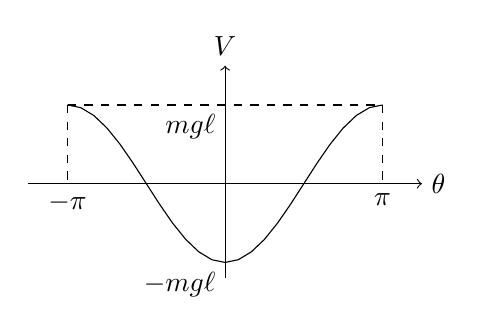
\begin{tikzpicture}
      \draw [domain=-1:1] plot ({2*\x}, {-1 * cos(180 * \x)});
      \draw [->] (-2.5, 0) -- (2.5, 0) node [right] {$\theta$};
      \draw [->] (0, -1.2) -- (0, 1.5) node [above] {$V$};
      \draw [dashed] (-2, 1) -- (-2, 0) node [below] {$-\pi$};
      \draw [dashed] (2, 1) -- (2, 0) node [below] {$\pi$};
      \draw [dashed] (-2, 1) -- (2, 1);
      \node [anchor = north east] at (0, 1) {$mg\ell$};
      \node [anchor = north east] at (0, -1) {$-mg\ell$};

    \end{tikzpicture}
  \end{center}
  If $E > mg\ell$, then $\dot{\theta}$ never vanishes and the pendulum makes full circles.

  If $0 < E < mg\ell$, then $\dot{\theta}$ vanishes at $\theta = \pm \theta_0$ for some $0 < \theta_0 < \pi$ i.e.\ $E = -mg\ell \cos\theta_0$. The pendulum oscillates back and forth. It takes a quarter of a period to reach from $\theta = 0$ to $\theta = \theta_0$. Using the previous general solution, oscillation period $P$ is given by
  \[
    \frac{P}{4} = \int_0^{\theta_0} = \frac{\d \theta}{\sqrt{\frac{2E}{m\ell^2} + \frac{2g}{\ell }\cos\theta}}.
  \]
  Since we know that $E = -mg\ell \cos \theta_0$, we know that
  \[
    \frac{P}{4} = \sqrt{\frac{\ell}{g}}\int_0^{\theta_0} \frac{\d \delta}{\sqrt{2\cos\theta - 2\cos\theta_0}}.
  \]
  The integral is difficult to evaluate in general, but for small $\theta_0$, we can use $\cos\theta \approx 1 - \frac{1}{2}\theta^2$. So
  \[
    P \approx 4\sqrt{\frac{\ell}{g}}\int_0^{\theta_0}\frac{\d \theta}{\sqrt{\theta_0^2 - \theta^2}} = 2\pi\sqrt{\frac{\ell}{g}}
  \]
  and is independent of the amplitude $\theta_0$. This is of course the result for the harmonic oscillator.
\end{eg}
\subsubsection*{Force and potential energy in three dimensions}
Everything looks nice so far. However, in real life, the world has (at least) three (spatial) dimensions. To work with multiple dimensions, we will have to promote our quantities into vectors.

Consider a particle of mass $m$ moving in 3D. The equation of motion is now a vector equation
\[
  m\ddot{\mathbf{r}} = \mathbf{F}.
\]
We'll define the familiar quantities we've had.
\begin{defi}[Kinetic energy]
  We define the \emph{kinetic energy} of the particle to be
  \[
    T = \frac{1}{2}m|\mathbf{v}|^2 = \frac{1}{2}m\dot{\mathbf{r}}\cdot \dot{\mathbf{r}}.
  \]
\end{defi}
If we want to know how it varies with time, we obtain
\[
  \frac{\d T}{\d t} = m\ddot{\mathbf{r}}\cdot \dot{\mathbf{r}} = \mathbf{F}\cdot \dot{\mathbf{r}} = \mathbf{F}\cdot \mathbf{v}.
\]
This is the power.
\begin{defi}[Power]
  The \emph{power} is the rate at which work is done on a particle by a force. It is given by
  \[
    P = \mathbf{F}\cdot \mathbf{v}.
  \]
\end{defi}
\begin{defi}[Work done]
  The \emph{work done} on a particle by a force is the change in kinetic energy caused by the force. The work done on a particle moving from $\mathbf{r}_1 = \mathbf{r}(t_1)$ to $\mathbf{r}_2 = \mathbf{r}(t_2)$ along a trajectory $C$ is the line integral
  \[
    W = \int_C \mathbf{F}\cdot\d \mathbf{r} = \int_{t_1}^{t_2} \mathbf{F}\cdot \dot{\mathbf{r}}\;\d t = \int_{t_1}^{t_2} P \;\d t.
  \]
\end{defi}
Usually, we are interested in forces that conserve energy. These are forces which can be given a potential, and are known as \emph{conservative forces}.
\begin{defi}[Conservative force and potential energy]
  A \emph{conservative force} is a force field $\mathbf{F}(\mathbf{r})$ that can be written in the form
  \[
    \mathbf{F} = -\nabla V.
  \]
  $V$ is the \emph{potential energy function}.
\end{defi}

\begin{prop}
  If $\mathbf{F}$ is conservative, then the energy
  \begin{align*}
    E &= T + V\\
    &= \frac{1}{2}m|\mathbf{v}|^2 + V(\mathbf{r})
  \end{align*}
  is conserved. For any particle moving under this force, the work done is equal to the change in potential energy, and is independent of the path taken between the end points. In particular, if we travel around a closed loop, no work is done.
\end{prop}

\begin{proof}
  \begin{align*}
    \frac{\d E}{\d t} &= \frac{\d}{\d t}\left(\frac{1}{2}m\dot{\mathbf{r}}\cdot \dot{\mathbf{r}} + V\right)\\
    &= m\ddot{\mathbf{r}}\cdot \dot{\mathbf{r}} + \frac{\partial V}{\partial x_i}\frac{\d x_i}{\d t}\\
    &= (m\ddot{\mathbf{r}} + \nabla V)\cdot \dot{\mathbf{r}}\\
    &= (m\ddot{\mathbf{r}} - \mathbf{F})\cdot \dot{\mathbf{r}}\\
    &= 0
  \end{align*}
  So the energy is conserved. In this case, the work done is
  \[
    W = \int_C \mathbf{F}\cdot \d \mathbf{r} = -\int_C (\nabla V)\cdot \d \mathbf{r} = V(\mathbf{r}_1) - V(\mathbf{r}_2).\qedhere
  \]
\end{proof}
\subsection{Central forces}
While in theory the potential can take any form it likes, most of the time, our system has \emph{spherical symmetry}. In this case, the potential depends only on the distance from the origin.
\begin{defi}[Central force]
  A \emph{central force} is a force with a potential $V(r)$ that depends only on the distance from the origin, $r = |\mathbf{r}|$. Note that a central force can be either attractive or repulsive.
\end{defi}

When dealing with central forces, the following formula is often helpful:
\begin{prop}
  $\nabla r = \hat{\mathbf{r}}$.
\end{prop}
Intuitively, this is because the direction in which $r$ increases most rapidly is $\mathbf{r}$, and the rate of increase is clearly 1. This can also be proved algebraically:

\begin{proof}
  We know that
  \[
    r^2 = x_1^2 + x_2^2 + x_3^2.
  \]
  Then
  \[
    2r\frac{\partial r}{\partial x_i} = 2x_i.
  \]
  So
  \[
    \frac{\partial r}{\partial x_i} = \frac{x_i}{r} = (\hat{\mathbf{r}})_i.\qedhere
  \]
\end{proof}

\begin{prop}
  Let $\mathbf{F} = -\nabla V(r)$ be a central force. Then
  \[
    \mathbf{F} = -\nabla V = -\frac{\d V}{\d r} \hat{\mathbf{r}},
  \]
  where $\hat{\mathbf{r}} = \mathbf{r}/r$ is the unit vector in the radial direction pointing away from the origin.
\end{prop}

\begin{proof}
  Using the proof above,
  \[
    (\nabla V)_i = \frac{\partial V}{\partial x_i} = \frac{\d V}{\d r} \frac{\partial r}{\partial x_i} = \frac{\d V}{\d r}(\hat{\mathbf{r}})_i\qedhere
  \]
\end{proof}
Since central forces have spherical symmetry, they give rise to an additional conserved quantity called \emph{angular momentum}.

\begin{defi}[Angular momentum]
  The \emph{angular momentum} of a particle is
  \[
    \mathbf{L} = \mathbf{r}\times \mathbf{p} = m\mathbf{r}\times \dot{\mathbf{r}}.
  \]
\end{defi}

\begin{prop}
  Angular momentum is conserved by a central force.
\end{prop}

\begin{proof}
  \[
    \frac{\d \mathbf{L}}{\d t} = m\dot{\mathbf{r}} \times \dot{\mathbf{r}} + m\mathbf{r}\times \ddot{\mathbf{r}} = \mathbf{0} + \mathbf{r}\times \mathbf{F} = \mathbf{0}.
  \]
  where the last equality comes from the fact that $\mathbf{F}$ is parallel to $\mathbf{r}$ for a central force.
\end{proof}
In general, for a non-central force, the rate of change of angular momentum is the \emph{torque}.
\begin{defi}[Torque]
  The \emph{torque} $G$ of a particle is the rate of change of angular momentum.
  \[
    \mathbf{G} = \frac{\d \mathbf{L}}{\d t} = \mathbf{r}\times \mathbf{F}.
  \]
\end{defi}

Note that $\mathbf{L}$ and $\mathbf{G}$ depends on the choice of origin. For a central force, only the angular momentum about the center of the force is conserved.

\subsection{Gravity}
We'll now study an important central force --- gravity. This law was discovered by Newton and was able to explain the orbits of various planets. However, we will only study the force and potential aspects of it, and postpone the study of orbits for a later time.

\begin{law}[Newton's law of gravitation]
  If a particle of mass $M$ is fixed at a origin, then a second particle of mass $m$ experiences a potential energy
  \[
    V(r) = -\frac{GMm}{r},
  \]
  where $G \approx \SI{6.67e-11}{\meter\cubed\per\kilogram\per\second\squared}$ is the \emph{gravitational constant}.

  The gravitational force experienced is then
  \[
    F = -\nabla V = -\frac{GMm}{r^2}\hat{\mathbf{r}}.
  \]
\end{law}
Since the force is negative, particles are attracted to the origin.

The potential energy is a function of the masses of \emph{both} the fixed mass $M$ and the second particle $m$. However, it is useful what the fixed mass $M$ does with reference to the second particle.
\begin{defi}[Gravitaional potential and field]
  The \emph{gravitational potential} is the gravitational potential energy per unit mass. It is
  \[
    \Phi_g(r) = -\frac{GM}{r}.
  \]
  Note that \emph{potential} is confusingly different from \emph{potential energy}.

  If we have a second particle, the potential \emph{energy} is given by $V = m\Phi_g$.

  The \emph{gravitational field} is the force per unit mass,
  \[
    \mathbf{g} = -\nabla \Phi_g = -\frac{GM}{r^2}\hat{\mathbf{r}}.
  \]
\end{defi}

If we have many fixed masses $M_i$ at points $\mathbf{r}_i$, we can add up their gravitational potential directly. Then the total gravitational potential is given by
\[
  \Phi_g(\mathbf{r}) = -\sum_i \frac{GM_i}{|\mathbf{r} - \mathbf{r}_i|}.
\]
Again, $V = m\Phi_g$ for a particle of mass $m$.

An important (mathematical) result about gravitational fields is that we can treat spherical objects as point particles. In particular,
\begin{prop}
  The external gravitational potential of a spherically symmetric object of mass $M$ is the same as that of a point particle with the same mass at the center of the object, i.e.
  \[
    \Phi_g(r) = -\frac{GM}{r}.
  \]
\end{prop}
The proof can be found in the Vector Calculus course.

\begin{eg}
  If you live on a spherical planet of mass $M$ and radius $R$, and can move only a small distance $z \ll R$ above the surface, then
  \begin{align*}
    V(r) &= V(R + z)\\
    &= -\frac{GMm}{R + z}\\
    &= -\frac{GMm}{R}\left(1 - \frac{z}{R} + \cdots\right)\\
    &\approx \text{const.} + \frac{GMm}{R^2}z\\
    &= \text{const.} + mgz,
  \end{align*}
  where $g = GM/R^2 \approx \SI{9.8}{\meter\per\second\squared}$ for Earth. Usually we are lazy and just say that the potential is $mgz$.
\end{eg}

\begin{eg}
  How fast do we need to jump to escape the gravitational pull of the Earth? If we jump upwards with speed $v$ from the surface, then
  \[
    E = T + V = \frac{1}{2}mv^2 - \frac{GMm}{R}.
  \]
  After escape, we must have $T \geq 0$ and $V = 0$. Since energy is conserved, we must have $E \geq 0$ from the very beginning. i.e.
  \[
    v > v_{esc} = \sqrt{\frac{2GM}{R}}.
  \]
\end{eg}
\subsubsection*{Inertial and gravitational mass}
A careful reader would observe that ``mass'' appears in two unrelated equations:
\[
  \mathbf{F} = m_i\ddot{\mathbf{r}}
\]
and
\[
  \mathbf{F} = -\frac{GM_gm_g}{r^2}\hat{\mathbf{r}},
\]
and they play totally different roles. The first is the \emph{inertial mass}, which measures the resistance to motion, while the second is the \emph{gravitational mass}, which measures its response to gravitational forces.

Conceptually, these are quite different. There is no \emph{a priori} reason why these two should be equal. However, experiment shows that they are indeed equivalent to each other, i.e.\ $m_i = m_g$, with an accuracy of $10^{-12}$ or better.

This (philosophical) problem was only resolved when Einstein introduced his general theory of relativity, which says that gravity is actually a \emph{fictitious} force, which means that the acceleration of the particle is independent of its mass.

We can further distinct the gravitational mass by ``passive'' and ``active'', i.e.\ the amount of gravitational field generated by a particle ($M$), and the amount of gravitational force received by a particle ($m$), but they are still equal, and we end up calling all of them ``mass''.
\subsection{Electromagnetism}
Next we will study the laws of electromagnetism. We will only provide a very rudimentary introduction to electromagnetism. Electromagnetism will be examined more in-depth in the IB Electromagnetism and II Electrodynamics courses.

As the name suggests, electromagnetism comprises two parts --- electricity and magnetism. Similar to gravity, we generally imagine electromagnetism working as follows: charges generate fields, and fields cause charges to move.

A common charged particle is the \emph{electron}, which is currently believed to be a fundamental particle. It has charge $q_e = \SI{-1.6e-19}{\coulomb}$. Other particles' charges are always integer multiples of $q_e$ (unless you are a quark).

In electromagnetism, there are two fields --- the \emph{electric field} $\mathbf{E}(\mathbf{r}, t)$ and the \emph{magnetic field} $\mathbf{B}(\mathbf{r}, t)$. Their effects on charged particles is described by the \emph{Lorentz force law}.
\begin{law}[Lorentz force law]
  The \emph{electromagnetic force} experienced by a particle with electric charge $q$ is
  \[
    \mathbf{F} = q(\mathbf{E} + \mathbf{v}\times \mathbf{B}).
  \]
\end{law}
This is the first time where we see a force that depends on the \emph{velocity} of the particle. In all other forces we've seen, the force depends only on the field which implicitly depends on the position only. This is weird, and seems to violate Galilean relativity, since velocity is a relative concept that depends on the frame of reference. It turns out that weird things happen to the $\mathbf{B}$ and $\mathbf{E}$ fields when you change the frame of reference. You will learn about these in the IB Electromagnetism course (if you take it).

As a result, the magnetic force is not a conservative force, and it cannot be given a (regular) potential. On the other hand, assuming that the fields are time-independent, the electric field \emph{is} conservative. We write the potential as $\Phi_e(\mathbf{r})$, and $\mathbf{E} = -\nabla \Phi_e$.

\begin{defi}[Electrostatic potential]
  The electrostatic potential is a function $\Phi_e(\mathbf{r})$ such that
  \[
    \mathbf{E} = -\nabla \Phi_e.
  \]
\end{defi}
While the magnetic force is not conservative in the traditional sense, it always acts perpendicularly to the velocity. Hence it does no work. So overall, energy is conserved under the action of the electromagnetic force.
\begin{prop}
  For time independent $\mathbf{E}(\mathbf{r})$ and $\mathbf{B}(\mathbf{r})$, the energy
  \[
    E = T + V = \frac{1}{2}m|\mathbf{v}|^2 + q\Phi_e
  \]
  is conserved.
\end{prop}

\begin{proof}
  \begin{align*}
    \frac{\d E}{\d t} &= m\ddot{\mathbf{r}}\cdot \dot{\mathbf{r}} + q(\nabla \Phi_e)\cdot \dot{\mathbf{r}}\\
    &= (m\ddot{\mathbf{r}} - q\mathbf{E}) \cdot \dot{\mathbf{r}}\\
    &= (q\dot{\mathbf{r}}\times \mathbf{B})\cdot \dot{\mathbf{r}}\\
    &= 0\qedhere
  \end{align*}
\end{proof}

\subsubsection*{Motion in a uniform magnetic field}
Consider the particular case where there is no electric field, i.e.\ $\mathbf{E} = \mathbf{0}$, and that the magnetic field is uniform throughout space. We choose our axes such that $\mathbf{B} = (0, 0, B)$ is constant.

According to the Lorentz force law, $\mathbf{F} = q(\mathbf{E} + \mathbf{v}\times \mathbf{B}) = q\mathbf{v}\times \mathbf{B}$. Since the force is always perpendicular to the velocity, we expect this to act as a centripetal force to make the particle travel in circles.

Indeed, writing out the components of the equation of motion, we obtain
\begin{align*}
  m\ddot{x} &= qB\dot{y}\tag{1}\\
  m\ddot{y} &= -qB\dot{x}\tag{2}\\
  m\ddot{z} &= 0\tag{3}
\end{align*}
From (3), we see that there is uniform motion parallel to $\mathbf{B}$, which is not interesting. We will look at the $x$ and $y$ components.

There are many ways to solve this system of equations. Here we solve it using complex numbers.

Let $\zeta = x + iy$. Then (1) + (2)$i$ gives
\[
  m\ddot{\zeta} = -iqB\dot{\zeta}.
\]
Then the solution is
\[
  \zeta = \alpha e^{-i\omega t} + \beta,
\]
where $\omega = qB/m$ is the \emph{gyrofrequency}, and $\alpha$ and $\beta$ are complex integration constants. We see that the particle goes in circles, with center $\beta$ and radius $\alpha$.

We can choose coordinates such that, at $t = 0$, $\mathbf{r} = 0$ and $\dot{\mathbf{r}} = (0, v, w)$, i.e.~$\zeta = 0$ and $\dot{\zeta} = iv$, and $z = 0$ and $\dot{z} = w$.

The solution is then
\[
  \zeta = R(1 - e^{-i\omega t}).
\]
with $R = v/\omega = (mv)/(qB)$ is the \emph{gyroradius} or \emph{Larmor radius}. Alternatively,
\begin{align*}
  x &= R(1 - \cos \omega t)\\
  y &= R\sin \omega t\\
  z &= wt.
\end{align*}
This is circular motion in the plane perpendicular to $\mathbf{B}$:
\[
  (x - R)^2 + y^2 = R^2,
\]
combined with uniform motion parallel to $\mathbf{B}$, i.e.~a helix.

Alternatively, we can solve this with vector operations. Start with
\[
  m\ddot{\mathbf{r}} = q\dot{\mathbf{r}}\times \mathbf{B}
\]
Let $\mathbf{B} = B\mathbf{n}$ with $|\mathbf{n}| = 1$. Then
\[
  \ddot{\mathbf{r}} = \omega \dot{\mathbf{r}}\times \mathbf{n},
\]
with our gyrofrequency $\omega = qB/m$. We integrate once, assuming $\mathbf{r}(0) = \mathbf{0}$ and $\dot{\mathbf{r}}(0) = \mathbf{v}_0$.
\[
  \dot{\mathbf{r}} = \omega \mathbf{r} \times \mathbf{n} + \mathbf{v}_0. \tag{$*$}
\]
Now we project $(*)$ parallel to and perpendicular to $\mathbf{B}$.

First we dot $(*)$ with $\mathbf{n}$:
\[
  \dot{\mathbf{r}}\cdot \mathbf{n} = \mathbf{v}_0\cdot \mathbf{n} = w = \text{const}.
\]
We integrate again to obtain
\[
  \mathbf{r}\cdot \mathbf{n} = wt.
\]
This is the part parallel to $\mathbf{B}$.

To resolve perpendicularly, write $\mathbf{r} = (\mathbf{r}\cdot \mathbf{n})\mathbf{n} + \mathbf{r}_\bot$, with $\mathbf{r}_\bot \cdot \mathbf{n} = 0$.

The perpendicular component of $(*)$ gives
\[
  \dot{\mathbf{r}}_\bot = w\mathbf{r}_\bot \times \mathbf{n} + \mathbf{v}_0 - (\mathbf{v}_0\cdot \mathbf{n})\mathbf{n}.
\]
We solve this by differentiating again to obtain
\[
  \ddot{\mathbf{r}}_\bot = \omega \dot{\mathbf{r}}_\bot \times \mathbf{n} = -\omega^2 \mathbf{r}_\bot + \omega \mathbf{v}_0 \times \mathbf{n},
\]
which we can solve using particular integrals and complementary functions.

\subsubsection*{Point charges}
So far we've discussed the effects of the fields on particles. But how can we create fields in the first place? We'll only look at the simplest case, where a point charge generates an electric field.

\begin{law}[Columb's law]
  A particle of charge $Q$, fixed at the origin, produces an electrostatic potential
  \[
    \Phi_e = \frac{Q}{4\pi\varepsilon_0 r},
  \]
  where $\varepsilon_0 \approx \SI{8.85e-12}{\per\meter\cubed\per\kilogram\second\squared\coulomb\squared}$.

  The corresponding electric field is
  \[
    \mathbf{E} = -\nabla \Phi_e = \frac{Q}{4\pi\varepsilon_0} \frac{\hat{\mathbf{r}}}{r^2}.
  \]
  The resulting force on a particle of charge $q$ is
  \[
    \mathbf{F} = q\mathbf{E} = \frac{Qq}{4\pi\varepsilon_0}\frac{\hat{\mathbf{r}}}{r^2}.
  \]
\end{law}
\begin{defi}[Electric constant]
  $\varepsilon_0$ is the \emph{electric constant} or \emph{vacuum permittivity} or \emph{permittivity of free space}.
\end{defi}

The form of equations here are closely analogous to those of gravity. However, there is an important difference: charges can be positive or negative. Thus electrostatic forces can be either attractive or repulsive, whereas gravity is always attractive.

\subsection{Friction}
At an atomic level, energy is always conserved. However, in many everyday processes, this does not appear to be the case. This is because \emph{friction} tends to take kinetic energy away from objects.

In general, we can divide friction into \emph{dry friction} and \emph{fluid friction}.
\subsubsection*{Dry friction}
When solid objects are in contact, a \emph{normal reaction force} $\mathbf{N}$ (perpendicular to the contact surface) prevents them from interpenetrating, while a \emph{frictional force} $\mathbf{F}$ (tangential to the surface) resists relative tangential motion (sliding or slipping).
\begin{center}
  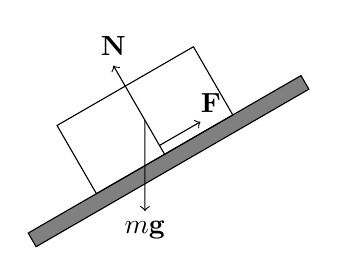
\begin{tikzpicture}[rotate = 30]
    \draw [fill=gray] (-2, 0) rectangle (2, -0.2);
    \draw (-1, 1) rectangle (1, 0);
    \draw [->] (0, 0) -- (0, 1.3) node [above] {$\mathbf{N}$};
    \draw [->] (0, 0.13) -- (0.6, 0.13) node [anchor = south west] {$\!\!\mathbf{F}$};
    \draw [->] (0, 0.5) -- (-0.577, -0.5) node [below] {$m\mathbf{g}$};
  \end{tikzpicture}
\end{center}
If the tangential force is small, it is insufficient to overcome friction and no sliding occurs. We have \emph{static friction} of
\[
  |\mathbf{F}| \leq \mu_s |\mathbf{N}|,
\]
where $\mu_s$ is the \emph{coefficient of static friction}.

When the external force on the object exceeds $\mu_s |\mathbf{N}|$, sliding starts, and we have a \emph{kinetic friction} of
\[
  |\mathbf{F}| = \mu_k |\mathbf{N}|,
\]
where $\mu_k$ is the \emph{coefficient of kinetic friction}.

These coefficients are measures of roughness and depend on the two surfaces involved. For example, Teflon on Teflon has coefficient of around 0.04, while rubber on asphalt has about 0.8, while a hypothetical perfectly smooth surface has coefficient $0$. Usually, $\mu_s > \mu_k > 0$.

\subsubsection*{Fluid drag}
When a solid object moves through a fluid (i.e.\ liquid or gas), it experiences a \emph{drag force}.

There are two important regimes.

\begin{enumerate}
  \item Linear drag: for small things in viscous fluids moving slowly, e.g.\ a single cell organism in water, the friction is proportional to the velocity, i.e.
    \[
      \mathbf{F} = -k_1 \mathbf{v}.
    \]
    where $\mathbf{v}$ is the velocity of the object relative to the fluid, and $k_1 > 0$ is a constant. This $k_1$ depends on the shape of the object. For example, for a sphere of radius $R$, Stoke's Law gives
    \[
      k_1 = 6\pi \mu R,
    \]
    where $\mu$ is the viscosity of the fluid.
  \item Quadratic drag: for large objects moving rapidly in less viscous fluid, e.g.\ cars or tennis balls in air, the friction is proportional to the square of the velocity, i.e.
    \[
      \mathbf{F} = -k_2|\mathbf{v}|^2\hat{\mathbf{v}}.
    \]
\end{enumerate}
In either case, the object loses energy. The power exerted by the drag force is
\[
  \mathbf{F}\cdot \mathbf{v} = \begin{cases} -k_1|\mathbf{v}|^2\\-k_2 |\mathbf{v}|^3 \end{cases}
\]
\begin{eg}
  Consider a projectile moving in a uniform gravitational field and experiencing a linear drag force.

  At $t = 0$, we throw the projectile with velocity $\mathbf{u}$ from $\mathbf{x} = \mathbf{0}$.

  The equation of motion is
  \[
    m\frac{\d \mathbf{v}}{\d t} = m\mathbf{g} - k\mathbf{v}.
  \]
  We first solve for $\mathbf{v}$, and then deduce $\mathbf{x}$.

  We use an integrating factor $\exp(\frac{k}{m}t)$ to obtain
  \begin{align*}
    \frac{\d }{\d t} \left(e^{kt/m}\mathbf{v}\right) &= e^{kt/m} \mathbf{g}\\
    e^{kt/m} \mathbf{v}&= \frac{m}{k}e^{kt/m}\mathbf{g} + \mathbf{c}\\
    \mathbf{v} &= \frac{m}{k}\mathbf{g} + \mathbf{c} e^{-kt/m}
  \end{align*}
  Since $\mathbf{v} = \mathbf{u}$ at $t = 0$, we get $\mathbf{c} = \mathbf{u} - \frac{m}{k}\mathbf{g}$. So
  \[
    \mathbf{v} = \dot{\mathbf{x}} = \frac{m}{k}\mathbf{g} + \left(\mathbf{u} - \frac{m}{k}\mathbf{g}\right)e^{-kt/m}.
  \]
  Integrating once gives
  \[
    \mathbf{x} = \frac{m}{k}\mathbf{g}t - \frac{m}{k}\left(\mathbf{u} - \frac{m}{k} \mathbf{g}\right) e^{-kt/m} + \mathbf{d}.
  \]
  Since $\mathbf{x} = \mathbf{0}$ at $t = 0$. So
  \[
    \mathbf{d} = \frac{m}{k}\left(\mathbf{u} - \frac{m}{k}\mathbf{g}\right).
  \]
  So
  \[
    \mathbf{x} = \frac{m}{k}\mathbf{g}t + \frac{m}{k}\left (\mathbf{u} - \frac{m}{k}\mathbf{g}\right)(1 - e^{-kt/m}).
  \]
  In component form, let $\mathbf{x} = (x, y)$, $\mathbf{u} = (u\cos \theta, u\sin \theta)$, $\mathbf{g} = (0, -g)$. So
  \begin{align*}
    x &= \frac{mu}{k}\cos \theta (1 - e^{-kt/m})\\
    y &= -\frac{mgt}{k} + \frac{m}{k}\left(u\sin \theta + \frac{mg}{k}\right)(1 - e^{-kt/m}).
  \end{align*}
  We can characterize the strength of the drag force by the dimensionless constant $ku/(mg)$, with a larger constant corresponding to a larger drag force.
\end{eg}
\subsubsection*{Effect of damping on small oscillations}
We've previously seen that particles near a potential minimum oscillate indefinitely. However, if there is friction in the system, the oscillation will damp out and energy is continually lost. Eventually, the system comes to rest at the stable equilibrium.

\begin{eg}
  If a linear drag force is added to a harmonic oscillator, then the equation of motion becomes
  \[
    m\ddot{\mathbf{x}} = -m\omega^2 \mathbf{x} - k\dot{\mathbf{x}},
  \]
  where $\omega$ is the angular frequency of the oscillator in the absence of damping. Rewrite as
  \[
    \ddot{\mathbf{x}} + 2\gamma \dot{\mathbf{x}} + \omega^2 x = 0,
  \]
  where $\gamma = k/2m > 0$. Solutions are $x = e^{\lambda t}$, where
  \[
    \lambda^2 + 2\gamma \lambda + \omega^2 = 0,
  \]
  or
  \[
    \lambda = -\gamma \pm \sqrt{\gamma^2 - \omega^2}.
  \]
  If $\gamma > \omega$, then the roots are real and negative. So we have exponential decay. We call this an overdamped oscillator.

  If $0 < \gamma < \omega$, then the roots are complex with $\Re(\lambda) = -\gamma$. So we have decaying oscillations. We call this an underdamped oscillator.

  For details, refer to Differential Equations.
\end{eg}

\section{Orbits}
The goal of this chapter is to study the orbit of a particle in a central force,
\[
  m\ddot{\mathbf{r}} = -\nabla V(r).
\]
While the universe is in three dimensions, the orbit is confined to a plane. This is since the angular momentum $\mathbf{L} = m\mathbf{r}\times \dot{\mathbf{r}}$ is a constant vector, as we've previously shown. Furthermore $\mathbf{L}\cdot \mathbf{r} = 0$. Therefore, the motion takes place in a plane passing through the origin, and perpendicular to $\mathbf{L}$.

\subsection{Polar coordinates in the plane}
We choose our axes such that the orbital plane is $z = 0$. To describe the orbit, we introduce polar coordinates $(r, \theta)$:
\[
  x = r\cos\theta, \quad y = r\sin \theta.
\]
Our object is to separate the motion of the particle into radial and angular components. We do so by defining unit vectors in the directions of increasing $r$ and increasing $\theta$:
\[
  \hat{\mathbf{r}} = \begin{pmatrix}\cos \theta\\ \sin \theta\end{pmatrix}, \quad \hat{\boldsymbol\theta} = \begin{pmatrix}-\sin \theta\\\cos\theta \end{pmatrix}.
\]
\begin{center}
  \begin{tikzpicture}
    \draw [->] (0, 0) -- (4, 0) node [right] {$x$};
    \draw [->] (0, 0) -- (0, 3) node [above] {$y$};
    \draw (0, 0) -- (2, 1.5) node [circ]{} node [pos = 0.5, anchor = south east] {$r$};
    \draw [->] (2, 1.5) -- (2.5, 1.875) node [anchor = south west] {$\hat{\mathbf{r}}$};
    \draw [->] (2, 1.5) -- (1.625, 2) node [anchor = south east] {$\hat{\boldsymbol\theta}$};
    \draw (0.7, 0) arc (0:36.87:0.7);
    \node at (0.9, 0.3) {$\theta$};
  \end{tikzpicture}
\end{center}
These two unit vectors form an orthonormal basis. However, they are not basis vectors in the normal sense. The directions of these basis vectors depend on time. In particular, we have

\begin{prop}
  \begin{align*}
    \frac{\d \hat{\mathbf{r}}}{\d \theta} &= \begin{pmatrix} -\sin \theta\\ \cos \theta\end{pmatrix} = \hat{\boldsymbol\theta}\\
    \frac{\d \hat{\boldsymbol\theta}}{\d \theta} &= \begin{pmatrix}-\cos \theta\\ -\sin \theta\end{pmatrix} = -\hat{\mathbf{r}}.
  \end{align*}
\end{prop}

Often, we want the derivative with respect to time, instead of $\theta$. By the chain rule, we have
\[
  \frac{\d \hat{\mathbf{r}}}{\d t} = \dot{\theta}\hat{\boldsymbol\theta},\quad \frac{\d \hat{\boldsymbol\theta}}{\d t} = -\dot{\theta} \hat{\mathbf{r}}.
\]
We can now express the position, velocity and acceleration in this new polar basis. The position is given by
\[
  \mathbf{r} = r\hat{\mathbf{r}}.
\]
Taking the derivative gives the velocity as
\[
  \dot{\mathbf{r}} = \dot{r} \hat{\mathbf{r}} + r\dot{\theta} \hat{\boldsymbol\theta}.
\]
The acceleration is then
\begin{align*}
  \ddot{\mathbf{r}} &= \ddot{r} \hat{\mathbf{r}} + \dot{r}\dot{\theta}\hat{\boldsymbol\theta} + \dot{r}\dot{\theta}\hat{\boldsymbol\theta} + r\ddot{\theta}\hat{\boldsymbol\theta} - r\dot{\theta}^2\hat{\mathbf{r}}\\
  &= (\ddot{r} - r\dot{\theta}^2)\hat{\mathbf{r}} + (r\ddot{\theta} + 2\dot{r}\dot{\theta})\hat{\boldsymbol\theta}.
\end{align*}
\begin{defi}[Radial and angular velocity]
  $\dot{r}$ is the \emph{radial velocity}, and $\dot{\theta}$ is the \emph{angular velocity}.
\end{defi}

\begin{eg}[Uniform motion in a circle]
  If we are moving in a circle, then $\dot{r} = 0$ and $\dot{\theta} = \omega = $ constant. So
  \[
    \dot{\mathbf{r}} = r\omega\hat{\boldsymbol\theta}.
  \]
  The speed is given by
  \[
  v = |\dot{\mathbf{r}}| = r|\omega| = \text{const}
  \]
  and the acceleration is
  \[
    \ddot{\mathbf{r}} = -r\omega^2 \hat{\mathbf{r}}.
  \]
  Hence in order to make a particle of mass $m$ move uniformly in a circle, we must supply a \emph{centripetal force} $mv^2/r$ towards the center.
\end{eg}

\subsection{Motion in a central force field}
Now let's put in our central force. Since $V = V(r)$, we have
\[
  \mathbf{F} = -\nabla V = \frac{\d V}{\d r} \hat{\mathbf{r}}.
\]
So Newton's 2nd law in polar coordinates is
\[
  m(\ddot{r} - r\dot{\theta}^2)\hat{\mathbf{r}} + m(r\ddot{\theta} + 2\dot{r}\dot{\theta})\hat{\boldsymbol\theta} = -\frac{\d V}{\d r}\hat{\mathbf{r}}.
\]
The $\theta$ component of this equation is
\[
  m(r\ddot{\theta} - 2\dot{r}\dot{\theta}) = 0.
\]
We can rewrite it as
\[
  \frac{1}{r}\frac{\d }{\d t}(mr^2 \dot{\theta}) = 0.
\]
Let $L = mr^2 \dot{\theta}$. This is the $z$ component (and the only component) of the conserved angular momentum $\mathbf{L}$:
\begin{align*}
  \mathbf{L} &= m\mathbf{r}\times \dot{\mathbf{r}}\\
  &= mr\hat{\mathbf{r}}\times (\dot{r}\hat{\mathbf{r}} + r\dot{\theta}\hat{\boldsymbol\theta})\\
  &= mr^2 \dot{\theta}\; \hat{\mathbf{r}}\times \hat{\boldsymbol\theta}\\
  &= mr^2 \dot{\theta}\; \hat{\mathbf{z}}.
\end{align*}
So the angular component tells us that $L$ is constant, which is the conservation of angular momentum.

However, a more convenient quantity is the angular momentum \emph{per unit mass}:
\begin{notation}[Angular momentum per unit mass]
  The \emph{angular momentum per unit mass} is
  \[
    h = \frac{L}{m} = r^2\dot\theta = \text{const.}
  \]
\end{notation}
Now the radial ($r$) component of the equation of motion is
\[
  m(\ddot{r} - r\dot{\theta}^2) = -\frac{\d V}{\d r}.
\]
We eliminate $\dot{\theta}$ using $r^2\dot{\theta} = h$ to obtain
\[
  m\ddot{r} = -\frac{\d V}{\d r} + \frac{mh^2}{r^3} = -\frac{\d V_{\text{eff}}}{\d r},
\]
where
\[
  V_{\text{eff}}(r) = V(r) + \frac{mh^2}{2r^2}.
\]
We have now reduced the problem to 1D motion in an (effective) potential --- as studied previously.

The total energy of the particle is
\begin{align*}
  E &= \frac{1}{2}m|\dot{\mathbf{r}}|^2 + V(r)\\
  &= \frac{1}{2}m(\dot{r}^2 + r^2\dot{\theta}^2) + V(r)\\
  \intertext{(since $\dot{\mathbf{r}} = \dot{r}\hat{\mathbf{r}} + r\dot{\theta}\hat{\boldsymbol\theta}$, and $\hat{\mathbf{r}}$ and $\hat{\boldsymbol\theta}$ are orthogonal)}
  &= \frac{1}{2}m\dot{r}^2 + \frac{mh^2}{2r^2} + V(r)\\
  &= \frac{1}{2}m\dot{r}^2 + V_{\text{eff}}(r).
\end{align*}

\begin{eg}
  Consider an attractive force following the inverse-square law (e.g.\ gravity). Here
  \[
    V = -\frac{mk}{r},
  \]
  for some constant $k$. So
  \[
    V_{\text{eff}} = -\frac{mk}{r} + \frac{mh^2}{2r^2}.
  \]
  We have two terms of opposite signs and different dependencies on $r$. For small $r$, the second term dominates and $V_{\text{eff}}$ is large. For large $r$, the first term dominates. Then $V_{\text{eff}}$ asymptotically approaches $0$ from below.
  \begin{center}
    \begin{tikzpicture}[xscale=0.5]
      \draw (0, 0) -- (8, 0) node [right] {$r$};
      \draw (0, -2) -- (0, 2) node [above] {$V_{\text{eff}}$};
      \draw [samples=70, domain=0.5:7.8] plot (\x, {-3/\x + 2/(\x*\x)});

      \draw [dashed] (1.33, -1.125) -- (0, -1.125) node [left] {$E_{\min}$};
      \draw [dashed] (1.33, -1.125) -- (1.33, 0) node [above] {$r_*$};
    \end{tikzpicture}
  \end{center}
  The minimum of $V_{\text{eff}}$ is at
  \[
    r_{*} = \frac{h^2}{k},\quad E_{\text{min}} = -\frac{mk^2}{2h^2}.
  \]
  We have a few possible types of motion:
  \begin{itemize}
    \item If $E = E_{\min}$, then $r$ remains at $r_*$ and $\dot{\theta} h/r^2$ is constant. So we have a uniform motion in a circle.
    \item If $E_{\min} < E < 0$, then $r$ oscillates and $\dot{r}=h/r^2$ does also. This is a non-circular, bounded orbit.

      We'll now introduce a lot of (pointless) definitions:

      \begin{defi}[Periapsis, apoapsis and apsides]
        The points of minimum and maximum $r$ in such an orbit are called the \emph{periapsis} and \emph{apoapsis}. They are collectively known as the \emph{apsides}.
      \end{defi}

      \begin{defi}[Perihelion and aphelion]
        For an orbit around the Sun, the periapsis and apoapsis are known as the \emph{perihelion} and \emph{aphelion}.
      \end{defi}

      In particular
      \begin{defi}[Perigee and apogee]
        The perihelion and aphelion of the Earth are known as the \emph{perigee} and \emph{apogee}.
      \end{defi}

    \item If $E \geq 0$, then $r$ comes in from $\infty$, reaches a minimum, and returns to infinity. This is an unbounded orbit.
  \end{itemize}

  We will later show that in the case of motion in an inverse square force, the trajectories are conic sections (circles, ellipses, parabolae and hyperbolae).
\end{eg}

\subsubsection*{Stability of circular orbits}
We'll now look at circular orbits, since circles are nice. Consider a general potential energy $V(r)$. We have to answer two questions:
\begin{itemize}
  \item Do circular orbits exist?
  \item If they do, are they stable?
\end{itemize}

The conditions for existence and stability are rather straightforward. For a circular orbit, $r = r_* =$ const for some value of $h\not= 0$ (if $h = 0$, then the object is just standing still!). Since $\ddot{r} = 0$ for constant $r$, we require
\[
  V'_{\text{eff}}(r_*) = 0.
\]
The orbit is stable if $r_*$ is a minimum of $V_{\text{eff}}$, i.e.
\[
  V_{\text{eff}}''(r_*) > 0.
\]
In terms of $V(r)$, circular orbit requires
\[
  V'(r_*) = \frac{mh^2}{r_*^3}
\]
and stability further requires
\[
  V''(r_*) + \frac{3mh^2}{r_*^4} = V''(r_*) + \frac{3}{r_*}V'(r_*) > 0.
\]
In terms of the radial force $F(r) = -V'(r)$, the orbit is stable if
\[
  F'(r_*) + \frac{3}{r}F(r_*) < 0.
\]
\begin{eg}
  Consider a central force with
  \[
    V(r) = -\frac{mk}{r^p}
  \]
  for some $k, p > 0$. Then
  \[
    V''(r) + \frac{3}{r}V'(r) = \big( -p(p + 1) + 3p\big)\frac{mk}{r^{p + 2}} = p(2-p)\frac{mk}{r^{p + 2}}.
  \]
  So circular orbits are stable for $p < 2$. This is illustrated by the graphs of $V_{\text{eff}}(r)$ for $p = 1$ and $p = 3$.
  \begin{center}
    \begin{tikzpicture}[xscale=0.5]
      \draw (0, 0) -- (8, 0);
      \draw (0, -2) -- (0, 2) node [above] {$V_{\text{eff}}$};
      \draw [blue, samples=10, domain=0.5:1.5] plot (\x, {-3/\x + 2/(\x*\x)});
      \draw [blue, domain=1.5:7.8] plot (\x, {-3/\x + 2/(\x*\x)}) node [right] {$p = 1$};


      \draw [red, dashed, samples=70, domain=0.4:7.8] plot (\x, {-0.6/(\x*\x*\x) + 1.2/(\x*\x)}) node [right] {$p = 3$};
    \end{tikzpicture}
  \end{center}
\end{eg}

\subsection{Equation of the shape of the orbit}
In general, we could determine $r(t)$ by integrating the energy equation
\begin{align*}
  E &= \frac{1}{2}m\dot{r}^2 + V_{\text{eff}}(r)\\
  t &= \pm \sqrt{\frac{m}{2}}\int \frac{\d r}{\sqrt{E - V_{\text{eff}}(r)}}
\end{align*}
However, this is usually not practical, because we can't do the integral. Instead, it is usually much easier to find the shape $r(\theta)$ of the orbit.

Still, solving for $r(\theta)$ is also not easy. We will need a magic trick --- we introduce the new variable
\begin{notation}
  \[
    u = \frac{1}{r}.
  \]
\end{notation}
Then
\[
  \dot{r} = \frac{\d r}{\d \theta}\dot{\theta} = \frac{\d r}{\d \theta}\frac{h}{r^2} = -h\frac{\d u}{\d \theta},
\]
and
\[
  \ddot{r} = \frac{\d }{\d t}\left(-h \frac{\d u}{\d \theta}\right) = -h\frac{\d ^2 u}{\d \theta^2}\dot{\theta} = -h\frac{\d ^2u}{\d \theta^2}\frac{h}{r^2} = -h^2u^2\frac{\d^2 u}{\d \theta^2}.
\]
This doesn't look very linear with $u^2$, but it will help linearizing the equation when we put in other factors.

The radial equation of motion
\[
  m\ddot{r} - \frac{mh^2}{r^3} = F(r)
\]
then becomes
\begin{prop}[Binet's equation]
  \[
    -mh^2u^2\left(\frac{\d^2u}{\d \theta^2}+ u\right) = F\left(\frac{1}{u}\right).
  \]
\end{prop}
This still looks rather complicated, but observe that for an inverse square force, $F(1/u)$ is proportional to $u^2$, and then the equation is linear!

In general, given an arbitrary $F(r)$, we aim to solve this second order ODE for $u(\theta)$. If needed, we can then work out the time-dependence via
\[
  \dot{\theta} = hu^2.
\]
\subsection{The Kepler problem}
The Kepler problem is the study of the orbits of two objects interacting via a central force that obeys the inverse square law. The goal is to classify the possible orbits and study their properties. One of the most important examples of the Kepler problem is the orbit of celestial objects, as studied by Kepler himself.
\subsubsection*{Shapes of orbits}
For a planet orbiting the sun, the potential and force are given by
\[
  V(r) = \frac{mk}{r},\quad F(r) = -\frac{mk}{r^2}
\]
with $k = GM$ (for the Coulomb attraction of opposite charges, we have the same equation with $\displaystyle k = -\frac{Qq}{4\pi\varepsilon_0 m}$).

Binet's equation then becomes linear, and
\[
  \frac{\d^2 u}{\d \theta^2} + u = \frac{k}{h^2}.
\]
We write the general solution as
\[
  u = \frac{k}{h^2} + A\cos(\theta - \theta_0),
\]
where $A \geq 0$ and $\theta_0$ are arbitrary constants.

If $A = 0$, then $u$ is constant, and the orbit is circular. Otherwise, $u$ reaches a maximum at $\theta = \theta_0$. This is the periapsis. We now re-define polar coordinates such that the periapsis is at $\theta = 0$. Then
\begin{prop}
  The orbit of a planet around the sun is given by
  \[
    r = \frac{\ell}{1 + e\cos \theta},\tag{$*$}
  \]
  with $\ell = h^2/k$ and $e = Ah^2/k$. This is the polar equation of a conic, with a focus (the sun) at the origin.
\end{prop}

\begin{defi}[Eccentricity]
  The dimensionless parameter $e \geq 0$ in the equation of orbit is the \emph{eccentricity} and determines the shape of the orbit.
\end{defi}

We can rewrite ($*$) in Cartesian coordinates with $x = r\cos \theta$ and $y = r\sin \theta$. Then we obtain
\[
  (1 - e^2)x^2 + 2e\ell x + y^2 = \ell^2.\tag{$\dagger$}
\]
There are three different possibilities:
\begin{itemize}
  \item Ellipse: ($0\leq e < 1$). $r$ is bounded by
    \[
      \frac{\ell}{1 + e} \leq r \leq \frac{\ell}{1 - e}.
    \]
    ($\dagger$) can be put into the equation of an ellipse centered on $(-ea, 0)$,
    \[
      \frac{(x + ea)^2}{a^2} + \frac{y^2}{b^2} = 1,
    \]
    where $\displaystyle a = \frac{\ell}{1 - e^2}$ and $\displaystyle b = \frac{\ell}{\sqrt{1 - e^2}}\leq a$.
    \begin{center}
      \begin{tikzpicture}
        \draw [gray] (-2, 0) -- (2, 0);
        \draw [gray] (0, -1.6) -- (0, 1.6);
        \draw [gray, ->] (0.7, -0.2) -- (0, -0.2) node [gray!50!black, pos = 0.5, below] {$ae$};
        \draw [gray, ->] (0, -0.2) -- (0.7, -0.2);
        \draw [gray, ->] (-0.2, 0) -- (-0.2, 1.6) node [gray!50!black, pos = 0.5, left] {$b$};
        \draw [gray, ->] (-0.2, 1.6) -- (-0.2, 0);

        \draw [gray, ->] (0, -0.2) -- (-2, -0.2) node [gray!50!black, pos = 0.5, below] {$a$};
        \draw [gray, ->] (-2, -0.2) -- (0, -0.2);
        \draw [gray, dashed] (0.7, 0) -- (0.7, 1.5) node [gray!50!black, pos = 0.5, right] {$\ell$};

        \draw (.7, 0) node [anchor = south west] {$O$} node [circ] {};
        \draw [->-=0.1] (0, 0) circle [x radius = 2, y radius = 1.6];
      \end{tikzpicture}
    \end{center}

    $a$ and $b$ are the semi-major and semi-minor axis. $\ell$ is the \emph{semi-latus rectum}. One focus of the ellipse is at the origin. If $e = 0$, then $a = b = \ell$ and the ellipse is a circle.

  \item Hyperbola: ($e > 1$). For $e > 1$, $r\to \infty$ as $\theta \to \pm \alpha$, where $\alpha = \cos^{-1}(1/e)\in (\pi/2, \pi)$. Then ($\dagger$) can be put into the equation of a hyperbola centered on $(ea, 0)$,
    \[
      \frac{(x - ea)^2}{a^2} - \frac{y^2}{b^2} = 1,
    \]
    with $\displaystyle a = \frac{\ell}{e^2 - 1}$, $\displaystyle b = \frac{\ell}{\sqrt{e^2 - 1}}$.
    \begin{center}
      \begin{tikzpicture}
        \draw [gray] (-3, -2) -- (3, 2);
        \draw [gray] (3, -2) -- (-3, 2);
        \draw [->-=0.3] (-3, -1.9) .. controls (-0.2, 0) .. (-3, 1.9);
        \draw [gray, ->] (0, 0) -- (-0.9, 0);
        \draw [gray, ->] (-0.9, 0) -- (0, 0) node [pos = 0.5, above] {$a$};
        \node at (-2, 0) [circ] {};
        \node at (-2, 0) [left] {$O$};
        \draw [gray, dashed] (-2, 0) -- (-2, 1.2) node [pos = 0.5, left] {$\ell$};
        \draw [gray, dashed] (-2, 0) -- (-1.38462, -0.923077) node [pos = 0.5, right] {$b$};
      \end{tikzpicture}
    \end{center}
    This corresponds to an unbound orbit that is deflected (scattered) by an attractive force.

    $b$ is both the semi-minor axis and the \emph{impact parameter}. It is the distance by which the planet would miss the object if there were no attractive force.

    The asymptote is $y = \frac{b}{a}(x - ea)$, or
    \[
      x \sqrt{e^2 - 1} - y = eb.
    \]
    Alternatively, we can write the equation of the asymptote as
    \[
      (x, y) \cdot \left(\frac{\sqrt{e^2 - 1}}{e}, -\frac{1}{e}\right) = b
    \]
    or $\mathbf{r} \cdot \mathbf{n} = b$, the equation of a line at a distance $b$ from the origin.

  \item Parabola: ($e = 1$). Then ($*$) becomes
    \[
      r = \frac{\ell}{1 + \cos \theta}.
    \]
    We see that $r\to \infty$ as $\theta \to \pm \pi$. ($\dagger$) becomes the equation of a parabola, $y^2 = \ell(\ell - 2x)$. The trajectory is similar to that of a hyperbola.
\end{itemize}

\subsubsection*{Energy and eccentricity}
We can figure out which path a planet follows by considering its energy.
\begin{align*}
  E &= \frac{1}{2}m(\dot{r}^2 + r^2\dot{\theta}^2) - \frac{mk}{r}\\
  &= \frac{1}{2}mh^2\left(\left(\frac{\d u}{\d \theta}\right)^2 + u^2\right) - mku
\end{align*}
Substitute $\displaystyle u = \frac{1}{\ell}(1 + e\cos \theta)$ and $\displaystyle \ell = \frac{h^2}{k}$, and it simplifies to
\[
  E = \frac{mk}{2\ell}(e^2 - 1),
\]
which is independent of $\theta$, as it must be.

Orbits are bounded for $e < 1$. This corresponds to the case $E < 0$. Unbounded orbits have $e > 1$ and thus $E > 0$. A parabolic orbit has $e = 1$, $E = 0$, and is ``marginally bound''.

Note that the condition $E > 0$ is equivalent to $|\dot{\mathbf{r}}| > \sqrt{\frac{2GM}{r}} = v_{\mathrm{esc}}$, which means you have enough kinetic energy to escape orbit.

\subsubsection*{Kepler's laws of planetary motion}
When Kepler first studied the laws of planetary motion, he took a telescope, observed actual planets, and came up with his famous three laws of motion. We are now going to derive the laws with pen and paper instead.

\begin{law}[Kepler's first law]
  The orbit of each planet is an ellipse with the Sun at one focus.
\end{law}

\begin{law}[Kepler's second law]
  The line between the planet and the sun sweeps out equal areas in equal times.
\end{law}

\begin{law}[Kepler's third law]
  The square of the orbital period is proportional to the cube of the semi-major axis, or
  \[
    P^2 \propto a^3.
  \]
\end{law}

We have already shown that Law 1 follows from Newtonian dynamics and the inverse-square law of gravity. In the solar system, planets generally have very low eccentricity (i.e.\ very close to circular motion), but asteroids and comets can have very eccentric orbits. In other solar systems, even planets have have highly eccentric orbits. As we've previously shown, it is also possible for the object to have a parabolic or hyperbolic orbit. However, we tend not to call these ``planets''.

Law 2 follows simply from the conservation of angular momentum: The area swept out by moving $\d \theta$ is $\d A = \frac{1}{2}r^2\;\d \theta$ (area of sector of circle). So
\[
  \frac{\d A}{\d t} = \frac{1}{2}r^2\dot{\theta} = \frac{h}{2} = \text{const}.
\]
and is true for \emph{any} central force.

Law 3 follows from this: the total area of the ellipse is $A = \pi ab = \frac{h}{2}P$ (by the second law). But $b^2 = a^2( 1 - e^2)$ and $h^2 = k\ell = ka(1 - e^2)$. So
\[
  P^2 = \frac{(2\pi)^2a^4(1 - e^2)}{ka(1 - e^2)} = \frac{(2\pi)^2 a^3}{k}.
\]
Note that the third law is very easy to prove directly for circular orbits. Since the radius is constant, $\ddot{r} = 0$. So the equations of motion give
\[
  -r \dot{\theta}^2 = -\frac{k}{r^2}
\]
So
\[
  r^3 \dot{\theta}^2 = k
\]
Since $\dot{\theta}\propto P^{-1}$, the result follows.

\subsection{Rutherford scattering}
Finally, we will consider the case where the force is \emph{repulsive} instead of attractive. An important example is the Rutherford gold foil experiment, where Rutherford bombarded atoms with alpha particles, and the alpha particles are repelled by the nucleus of the atom.

Under a repulsive force, the potential and force are given by
\[
  V(r) = +\frac{mk}{r}, \quad F(r) = +\frac{mk}{r^2}.
\]
For Coulomb repulsion of like charges,
\[
  k = \frac{Qq}{4\pi \varepsilon_0 m} > 0.
\]
The solution is now
\[
  u = -\frac{k}{h^2} + A\cos (\theta - \theta_0).
\]
wlog, we can take $A \geq 0, \theta_0 = 0$. Then
\[
  r = \frac{\ell}{e\cos \theta - 1}
\]
with
\[
  \ell = \frac{h^2}{k}, \quad e = \frac{Ah^2}{k}.
\]
We know that $r$ and $\ell$ are positive. So we must have $e \geq 1$. Then $r\to \infty$ as $\theta \to \pm \alpha$, where $\alpha = \cos^{-1}(1/e)$.

The orbit is a hyperbola, again given by
\[
  \frac{(x - ea)^2}{a^2} - \frac{y^2}{b^2} = 1,
\]
with $a = \frac{\ell}{e^2 - 1}$ and $b = \frac{\ell}{\sqrt{e^2 - 1}}$. However, this time, the trajectory is the other branch of the hyperbola.
\begin{center}
  \begin{tikzpicture}
    \draw [gray] (-3, -2) -- (3, 2);
    \draw [gray] (3, -2) -- (-3, 2);
    \draw [->-=0.3] (3, -1.9) .. controls (0.2, 0) .. (3, 1.9);
    \node at (-2, 0) [circ] {};
    \node at (-2, 0) [left] {$O$};
    \draw [dashed] (-2, 0) -- (-1.38462, 0.923077) node [pos = 0.5, right] {$b$};
    \draw (0.3, 0) arc (0:-33:0.3);
    \draw (0.3, 0) arc (0:33:0.3);
    \node at (0.3, 0) [right] {$2\alpha$};
    \draw (0, 0.4) arc (90:33:0.4);
    \draw (0, 0.4) arc (90:147:0.4);
    \node at (0, 0.4) [above] {$\beta$};
  \end{tikzpicture}
\end{center}
It seems as if the particle is deflected by $O$.

We can characterize the path of the particle by the impact parameter $b$ and the incident speed $v$ (i.e.\ the speed when far away from the origin). We know that the angular momentum per unit mass is $h = bv$ (velocity $\times$ perpendicular distance to $O$).

How does the scattering angle $\beta = \pi - 2\alpha$ depend on the impact parameter $b$ and the incident speed $v$?

Recall that the angle $\alpha$ is given by $\alpha = \cos^{-1} (1/e)$. So we obtain
\[
  \frac{1}{e} = \cos \alpha = \cos \left(\frac{\pi}{2} - \frac{\beta}{2}\right) = \sin\left(\frac{\beta}{2}\right),
\]
So
\[
  b = \frac{\ell}{\sqrt{e^2 - 1}} = \frac{(bv)^2}{k}\tan \frac{\beta}{2}.
\]
So
\[
  \beta = 2\tan^{-1}\left(\frac{k}{bv^2}\right).
\]
We see that if we have a small impact parameter, i.e.\ $b \ll k/v^2$, then we can have a scattering angle approaching $\pi$.

\section{Rotating frames}
Recall that Newton's laws hold only in inertial frames. However, sometimes, our frames are not inertial. In this chapter, we are going to study a particular kind of non-inertial frame --- a rotating frame. An important rotating frame is the Earth itself, but there are also other examples such as merry-go-rounds.

\subsection{Motion in rotating frames}
Now suppose that $S$ is an inertial frame, and $S'$ is rotating about the $z$ axis with angular velocity $\omega = \dot{\theta}$ with respect to $S$.

\begin{defi}[Angular velocity vector]
  The \emph{angular velocity vector} of a rotating frame is $\boldsymbol\omega = \omega\hat{\mathbf{z}}$, where $\hat{\mathbf{z}}$ is the axis of rotation and $\omega$ is the angular speed.
\end{defi}

First we wish to relate the basis vectors $\{\mathbf{e}_i\}$ and $\{\mathbf{e}_i'\}$ of $S$ and $S'$ respectively.

Consider a particle at rest in $\mathbf{S}'$. From the perspective of $S$, its velocity is
\[
  \left(\frac{\d \mathbf{r}}{\d t}\right)_S = \boldsymbol\omega\times \mathbf{r},
\]
where $\boldsymbol\omega = \omega\hat{\mathbf{z}}$ is the \emph{angular velocity vector} (aligned with the rotation axis). This formula also applies to the basis vectors of $S'$.
\[
  \left(\frac{\d \mathbf{e}_i'}{\d t}\right)_S = \boldsymbol\omega\times \mathbf{e}_i'.
\]
Now given a general time-dependent vector $\mathbf{a}$, we can express it in the $\{\mathbf{e}_i'\}$ basis as follows:
\[
  \mathbf{a} = \sum a_i'(t) \mathbf{e}_i'.
\]
From the perspective of $S'$, $\mathbf{e}_i'$ is constant and the time derivative of $\mathbf{a}$ is given by
\[
  \left(\frac{\d \mathbf{a}}{\d t}\right)_{S'} = \sum \frac{\d a_i'}{\d t}\mathbf{e}_i'.
\]
In $S$, however, $\mathbf{e}_i'$ is not constant. So we apply the product rule to obtain the time derivative of $\mathbf{a}$:
\[
  \left(\frac{\d \mathbf{a}}{\d t}\right)_S = \sum \frac{\d a_i}{\d t}\mathbf{e}_i' + \sum a_i'\boldsymbol\omega \times \mathbf{e}_i' = \left(\frac{\d \mathbf{a}}{\d t}\right)_{S'} + \boldsymbol\omega \times \mathbf{a}.
\]
This key identity applies to all vectors and can be written as an operator equation:
\begin{prop}
  If $S$ is an inertial frame, and $S'$ is rotating relative to $S$ with angular velocity $\boldsymbol \omega$, then
  \[
    \left(\frac{\d}{\d t}\right)_S = \left(\frac{\d}{\d t}\right)_{S'} + \boldsymbol\omega \times.
  \]
  Applied to the position vector $\mathbf{r}(t)$ of a particle, it gives
  \[
    \left(\frac{\d \mathbf{r}}{\d t}\right)_S = \left(\frac{\d \mathbf{r}}{\d t}\right)_{S'} + \boldsymbol\omega \times \mathbf{r}.
  \]
\end{prop}
We can interpret this as saying that the difference in velocity measured in the two frames is the relative velocity of the frames.

We apply this formula a second time, and allow $\boldsymbol\omega$ to depend on time. Then we have
\begin{align*}
  \left(\frac{\d ^2\mathbf{r}}{\d t^2}\right)_S &= \left(\left(\frac{\d }{\d t}\right)_{S'} + \boldsymbol\omega\times \right)\left(\left(\frac{\d \mathbf{r}}{\d t}\right)_{S'} + \boldsymbol\omega \times \mathbf{r}\right).\\
  &= \left(\frac{\d^2 \mathbf{r}}{\d t^2}\right)_{S'} + 2\boldsymbol \omega \times \left(\frac{\d \mathbf{r}}{\d t}\right)_{S'} + \dot{\boldsymbol\omega} \times \mathbf{r} + \boldsymbol\omega\times(\boldsymbol\omega\times \mathbf{r})
\end{align*}
Since $S$ is inertial, Newton's Second Law is
\[
  m\left(\frac{\d ^2\mathbf{r}}{\d t^2}\right)_S = \mathbf{F}.
\]
So
\begin{prop}
  \[
    m\left(\frac{\d^2 \mathbf{r}}{\d t^2}\right)_{S'} = \mathbf{F} - 2m\boldsymbol\omega \times \left(\frac{\d \mathbf{r}}{\d t}\right)_{S'} - m\dot{\boldsymbol\omega}\times \mathbf{r} - m\boldsymbol\omega \times (\boldsymbol\omega \times \mathbf{r}).
  \]
\end{prop}

\begin{defi}[Fictious forces]
  The additional terms on the RHS of the equation of motion in rotating frames are \emph{fictitious forces}, and are needed to explain the motion observed in $S'$. They are
  \begin{itemize}
    \item \emph{Coriolis force}: $-2m\boldsymbol\omega \times \left(\frac{\d \mathbf{r}}{\d t}\right)_{S'}.$
    \item \emph{Euler force}: $-m\dot{\boldsymbol\omega}\times \mathbf{r}$
    \item \emph{Centrifugal force}: $-m\boldsymbol\omega\times(\boldsymbol\omega\times \mathbf{r})$.
  \end{itemize}
\end{defi}
In most cases, $\boldsymbol \omega$ is constant and can neglect the Euler force.
\subsection{The centrifugal force}
What exactly does the centrifugal force do? Let $\boldsymbol\omega = \omega\hat{\boldsymbol\omega}$, where $|\hat{\boldsymbol\omega}| = 1$. Then
\[
  -m\boldsymbol\omega \times (\boldsymbol\omega \times \mathbf{r}) = -m\big((\boldsymbol\omega \cdot \mathbf{r})\boldsymbol\omega - (\boldsymbol\omega \cdot \boldsymbol\omega)\mathbf{r}\big) = m\omega^2 \mathbf{r}_{\bot},
\]
where $\mathbf{r}_{\bot} = \mathbf{r} - (\mathbf{r}\cdot \hat{\boldsymbol\omega})\hat{\boldsymbol\omega}$ is the projection of the position on the plane perpendicular to $\boldsymbol\omega$. So the centrifugal force is directed away from the axis of rotation, and its magnitude is $m\omega^2$ times the distance form the axis.
\begin{center}
  \begin{tikzpicture}
    \draw [->] (0, 0) -- (0, 3) node [above] {$\boldsymbol\omega$};
    \draw [->] (-0.15, 2.5) arc (120:420:0.3 and 0.1);
    \draw [->] (0, 0.5) -- (1.5, 1.5) node [pos=0.5, anchor = north west] {$\mathbf{r}$};
    \draw [->] (0, 1.5) -- (1.5, 1.5) node [pos = 0.5, above] {$\mathbf{r}_\bot$};
  \end{tikzpicture}
\end{center}
Note that
\begin{align*}
  \mathbf{r}_\bot \cdot \mathbf{r}_\bot &= \mathbf{r}\cdot \mathbf{r} - (\mathbf{r} \cdot \hat{\boldsymbol\omega})^2\\
  \nabla(|\mathbf{r}_\bot|^2) &= 2\mathbf{r} - 2(\mathbf{r}\cdot \hat{\boldsymbol\omega})\hat{\boldsymbol\omega} = 2\mathbf{r}_\bot.
\end{align*}
So
\[
  -m\boldsymbol\omega\times(\boldsymbol\omega\times \mathbf{r}) = -\nabla\left(-\frac{1}{2}m\omega^2|\mathbf{r}_\bot|^2\right) = -\nabla\left(-\frac{1}{2}m|\boldsymbol\omega\times \mathbf{r}|^2\right).
\]
Thus the centrifugal force is a conservative (fictitious) force.

On a rotating planet, the gravitational and centrifugal forces per unit mass combine to make the \emph{effective gravity},
\[
  \mathbf{g}_{\text{eff}} = \mathbf{g} + \omega^2 \mathbf{r}_\bot.
\]
This gravity will not be vertically downwards. Consider a point $P$ at latitude $\lambda$ on the surface of a spherical planet of radius $R$.

We construct orthogonal axes:
\begin{center}
  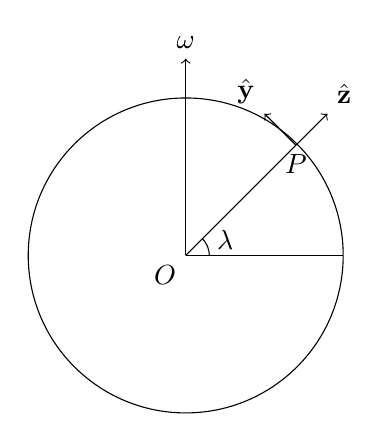
\begin{tikzpicture}
    \draw circle [radius = 2];
    \node [anchor = north east] {$O$};
    \draw [->] (0, 0) -- (0, 2.5) node [above] {$\boldsymbol\omega$};
    \draw (0, 0) -- (2, 0);
    \draw (0, 0) -- (1.4, 1.4) node [below] {$P$};
    \draw [->] (1.4, 1.4) -- (1.8, 1.8) node [anchor = south west] {$\hat{\mathbf{z}}$};
    \draw [->] (1.4, 1.4) -- (1, 1.8) node [anchor = south east] {$\hat{\mathbf{y}}$};
    \draw (0.3, 0) arc (0:45:0.3);
    \node at (0.5, 0.2) {$\lambda$};
  \end{tikzpicture}
\end{center}
with $\hat{\mathbf{x}}$ into the page. So $\hat{\mathbf{z}}$ is up, $\hat{\mathbf{y}}$ is North, and $\hat{\mathbf{x}}$ is East.

At $P$, we have
\begin{align*}
  \mathbf{r} &= R\hat{\mathbf{z}}\\
  \mathbf{g} &= -g\hat{\mathbf{z}}\\
  \boldsymbol\omega &= \omega(\cos\lambda \hat{\mathbf{y}} + \sin \lambda \hat{\mathbf{z}})
\end{align*}
So
\begin{align*}
  \mathbf{g}_{\mathrm{eff}} &= \mathbf{g} + \omega^2 \mathbf{r}_\bot \\
  &= -g\hat{\mathbf{z}} + \omega^2 R\cos\lambda(\cos\lambda\hat{\mathbf{z}} - \sin\lambda\hat{\mathbf{y}})\\
  &= -\omega^2 R\cos\lambda\sin\lambda\hat{\mathbf{y}} - (g - \omega^2 R\cos^2\lambda)\hat{\mathbf{z}}.
\end{align*}
So the angle $\alpha$ between $\mathbf{g}$ and $\mathbf{g}_{\text{eff}}$ is given by
\[
  \tan \alpha = \frac{\omega^2 R\cos\lambda\sin\lambda}{g - \omega^2R\cos^2\lambda}.
\]
This is 0 at the equator and the poles, and greatest when you are halfway between. However, this is still tiny on Earth, and does not affect our daily life.

\subsection{The Coriolis force}
The Coriolis force is a more subtle force. Writing $\mathbf{v} = \left(\frac{\d \mathbf{r}}{\d t}\right)_{S'}$, we can write the force as
\[
  \mathbf{F} = -2m\boldsymbol\omega\times \mathbf{v}.
\]
Note that this has the same form as the Lorentz force caused by a magnetic field, and is velocity-dependent. However, unlike the effects of a magnetic field, particles do not go around in circles in a rotating frame, since we also have the centrifugal force in play.

Since this force is always perpendicular to the velocity, it does no work.

Consider motion parallel to the Earth's surface. We only care about the effect of the Coriolis force on the horizontal trajectory, and ignore the vertical component that is tiny compared to gravity.

So we only take the vertical component of $\boldsymbol\omega$, $\omega\sin\lambda\hat{\mathbf{z}}$. The horizontal velocity $\mathbf{v} = v_x \hat{\mathbf{x}} + v_y \hat{\mathbf{y}}$ generates a horizontal Coriolis force:
\[
  -2m\omega\sin\lambda\hat{\mathbf{z}}\times \mathbf{v} = -2m\omega\sin\lambda(v_y \hat{\mathbf{x}} - v_x \hat{\mathbf{y}}).
\]
In the Northern hemisphere $(0 < \lambda < \pi/2)$, this causes a deflection towards the right. In the Southern Hemisphere, the deflection is to the left. The effect vanishes at the equator.

Note that only the horizontal effect of horizontal motion vanishes at the equator. The vertical effects or those caused by vertical motion still exist.

\begin{eg}
  Suppose a ball is dropped from a tower of height $h$ at the equator. Where does it land?

  In the rotating frame,
  \[
    \ddot{\mathbf{r}} = \mathbf{g} - 2\boldsymbol\omega\times \dot{\mathbf{r}} - \boldsymbol\omega\times(\boldsymbol\omega\times \mathbf{r}).
  \]
  We work to first order in $\omega$. Then
  \[
    \ddot{\mathbf{r}} = \mathbf{g} - 2\boldsymbol\omega\times \dot{\mathbf{r}} + O(\omega^2).
  \]
  Integrate wrt $t$ to obtain
  \[
    \dot{\mathbf{r}} = \mathbf{g}t - 2\boldsymbol\omega \times (\mathbf{r} - \mathbf{r}_0) + O(\omega^2),
  \]
  where $\mathbf{r}_0$ is the initial position. We substitute into the original equation to obtain
  \[
    \ddot{\mathbf{r}} = \mathbf{g} - 2\boldsymbol\omega\times \mathbf{g}t + O(\omega^2).
  \]
  (where some new $\omega^2$ terms are thrown into $O(\omega^2)$). We integrate twice to obtain
  \[
    \mathbf{r} = \mathbf{r}_0 + \frac{1}{2}\mathbf{g}t^2 - \frac{1}{3}\boldsymbol\omega \times \mathbf{g}t^3 + O(\omega^2).
  \]
  In components, we have $\mathbf{g} = (0, 0, -g)$, $\boldsymbol\omega = (0, \omega, 0)$ and $\mathbf{r}_0 = (0, 0, R + h)$. So
  \[
    \mathbf{r} = \left(\frac{1}{3}\omega gt^3, 0, R + h - \frac{1}{2}gt^2\right) + O(\omega^2).
  \]
  So the particle hits the ground at $t = \sqrt{2h/g}$, and its eastward displacement is $\frac{1}{3}wg\left(\frac{2h}{g}\right)^{3/2}$.

  This can be understood in terms of angular momentum conservation in the non-rotating frame. At the beginning, the particle has the same angular velocity with the Earth. As it falls towards the Earth, to maintain the same angular momentum, the angular velocity has to increase to compensate for the decreased radius. So it spins faster than the Earth and drifts towards the East, relative to the Earth.
\end{eg}

\begin{eg}
  Consider a pendulum that is free to swing in any plane, e.g.\ a weight on a string. At the North pole, it will swing in a plane that is fixed in an inertial frame, while the Earth rotates beneath it. From the perspective of the rotating frame, the plane of the pendulum rotates backwards. This can be explained as a result of the Coriolis force.

  In general, at latitude $\lambda$, the plane rotates rightwards with period $\frac{1\text{ day}}{\sin \lambda}$.
\end{eg}

\section{Systems of particles}
Now suppose we have $N$ interacting particles. We adopt the following notation: particle $i$ has mass $m_i$, position $\mathbf{r}_i$, and momentum $\mathbf{p}_i = m_i \dot{\mathbf{r}}_i$. Note that the subscript denotes which particle it is referring to, not vector components.

Newton's Second Law for particle $i$ is
\[
  m_i \ddot{\mathbf{r}}_i = \dot{\mathbf{p}}_i = \mathbf{F}_i,
\]
where $\mathbf{F}_i$ is the total force acting on particle $i$. We can write $\mathbf{F}_i$ as
\[
  \mathbf{F}_i = \mathbf{F}_i^{\text{ext}} + \sum_{j = 1}^N \mathbf{F}_{ij},
\]
where $\mathbf{F}_{ij}$ is the force on particle $i$ by particle $j$, and $\mathbf{F}_i^{\text{ext}}$ is the external force on $i$, which comes from particles outside the system.

Since a particle cannot exert a force on itself, we have $\mathbf{F}_{ii} = \mathbf{0}$. Also, Newton's third law requires that
\[
  \mathbf{F}_{ij} = -\mathbf{F}_{ji}.
\]
For example, if the particles interact only via gravity, then we have
\[
  \mathbf{F}_{ij} = -\frac{Gm_im_j(\mathbf{r}_i - \mathbf{r}_j)}{|\mathbf{r}_i - \mathbf{r}_j|^3} = -\mathbf{F}_{ji}.
\]
\subsection{Motion of the center of mass}
Sometimes, we are interested in the collection of particles as a whole. For example, if we treat a cat as a collection of particles, we are more interested in how the cat as a whole falls, instead of tracking the individual particles of the cat.

Hence, we define some aggregate quantities of the system such as the total mass and investigate how these quantities relate.
\begin{defi}[Total mass]
  The \emph{total mass} of the system is $M = \sum m_i$.
\end{defi}

\begin{defi}[Center of mass]
  The \emph{center of mass} is located at
  \[
    \mathbf{R} = \frac{1}{M}\sum_{i = 1}^N m_i\mathbf{r}_i.
  \]
  This is the mass-weighted average position.
\end{defi}

\begin{defi}[Total linear momentum]
  The \emph{total linear momentum} is
  \[
    \mathbf{P} = \sum_{i = 1}^N \mathbf{p}_i = \sum_{i = 1}^N m_i \dot{\mathbf{r}}_i = M\dot{\mathbf{R}}.
  \]
  Note that this is equivalent to the momentum of a single particle of mass $M$ at the center of mass.
\end{defi}

\begin{defi}[Total external force]
  The \emph{total external force} is
  \[
    \mathbf{F} = \sum_{i = 1}^N \mathbf{F}_i^{\text{ext}}.
  \]
\end{defi}

We can now obtain the equation of motion of the center of mass:
\begin{prop}
  \[
    M\ddot{\mathbf{R}} = \mathbf{F}.
  \]
\end{prop}

\begin{proof}
  \begin{align*}
    M\ddot{\mathbf{R}} &= \dot{\mathbf{P}}\\
    &= \sum_{i = 1}^N \dot{\mathbf{p}}_i\\
    &= \sum_{i = 1}^N \mathbf{F}_i^{\text{ext}} + \sum_{i = 1}^N\sum_{j = 1}^N \mathbf{F}_{ij}\\
    &= \mathbf{F} + \frac{1}{2}\sum_i \sum_j(\mathbf{F}_{ij} + \mathbf{F}_{ji})\\
    &= \mathbf{F}\qedhere
  \end{align*}
\end{proof}
This means that if we don't care about the internal structure, we can treat the system as a point particle of mass $M$ at the center of mass $\mathbf{R}$. This is why Newton's Laws apply to macroscopic objects even though they are not individual particles.

\begin{law}[Conservation of momentum]
  If there is no external force, i.e.\ $\mathbf{F} = \mathbf{0}$, then $\dot{\mathbf{P}} = \mathbf{0}$. So the total momentum is conserved.
\end{law}

If there is no external force, then the center of mass moves uniformly in a straight line. In this case, we can pick a particularly nice frame of reference, known as the \emph{center of mass frame}.
\begin{defi}[Center of mass frame]
  The \emph{center of mass frame} is an inertial frame in which $\mathbf{R} = 0$ for all time.
\end{defi}
Doing calculations in the center of mass frame is usually much more convenient than using other frames,

After doing linear motion, we can now look at angular motion.
\begin{defi}[Total angular momentum]
  The \emph{total angular momentum} of the system about the origin is
  \[
    \mathbf{L} = \sum_i \mathbf{r}_i \times \mathbf{p}_i.
  \]
\end{defi}
How does the total angular momentum change with time? Here we have to assume a stronger version of Newton's Third law, saying that
\[
  \mathbf{F}_{ij} = -\mathbf{F}_{ji}\text{ and is parallel to }(\mathbf{r}_i - \mathbf{r}_j).
\]
This is true, at least, for gravitational and electrostatic forces.

Then we have
\begin{align*}
  \dot{\mathbf{L}} &= \sum_i \mathbf{r}_i \times \dot{\mathbf{p}}_i + \dot{\mathbf{r}}_i \times \mathbf{p}_i\\
  &= \sum_i \mathbf{r}_i \times \left(\mathbf{F}_i^{\text{ext}} + \sum_j F_{ij}\right) + m(\dot{\mathbf{r}}_i\times \dot{\mathbf{r}}_i)\\
  &= \sum_i \mathbf{r}_i\times \mathbf{F}_i^{\text{ext}} + \sum_i \sum_j \mathbf{r}_i \times \mathbf{F}_{ij}\\
  &= \sum_i \mathbf{G}_i^{\text{ext}} + \frac{1}{2}\sum_i\sum_j (\mathbf{r}_i \times \mathbf{F}_{ij} + \mathbf{r}_j\times \mathbf{F}_{ji})\\
  &= \mathbf{G} + \frac{1}{2}\sum_i\sum_j(\mathbf{r}_i - \mathbf{r}_j)\times \mathbf{F}_{ij}\\
  &= \mathbf{G},
\end{align*}
where
\begin{defi}[Total external torque]
  The \emph{total external torque} is
  \[
    \mathbf{G} = \sum_i \mathbf{r}_i \times \mathbf{F}_i^{\text{ext}}.
  \]
\end{defi}
So the total angular momentum is conserved if $\mathbf{G} = \mathbf{0}$, ie the total external torque vanishes.

\subsection{Motion relative to the center of mass}
So far, we have shown that externally, a multi-particle system behaves as if it were a point particle at the center of mass. But internally, what happens to the individual particles themselves?

We write $\mathbf{r}_i = \mathbf{R} + \mathbf{r}_i^c$, where $\mathbf{r}_i^c$ is the position of particle $i$ relative to the center of mass.

We first obtain two useful equalities:
\[
  \sum_i m_i\mathbf{r}_i^c = \sum m_i \mathbf{r}_i - \sum m_i \mathbf{R} = M\mathbf{R} - M\mathbf{R} = \mathbf{0}.
\]
Differentiating gives
\[
  \sum_i m_i \dot{\mathbf{r}}_i^c = \mathbf{0}.
\]
Using these equalities, we can express the angular momentum and kinetic energy in terms of $\mathbf{R}$ and $\mathbf{r}_i^c$ only:
\begin{align*}
  \mathbf{L} &= \sum_i m_i(\mathbf{R} + \mathbf{r}_i^c) \times (\dot{\mathbf{R}} + \dot{\mathbf{r}}_i^c)\\
  &= \sum_i m_i \mathbf{R}\times \dot{\mathbf{R}} + \mathbf{R}\times \sum_i m_i \dot{\mathbf{r}}_i^c + \sum_i m_i \mathbf{r}_i^c\times \dot{\mathbf{R}} + \sum_i m_i \mathbf{r}_i^c \times \dot{\mathbf{r}}_i^c\\
  &= M\mathbf{R}\times \dot{\mathbf{R}} + \sum_i m_i \mathbf{r}_i^c \times \dot{\mathbf{r}}_i^c\displaybreak[0]\\
  T&= \frac{1}{2}\sum_i m_i|\dot{\mathbf{r}}_i|^2\\
  &= \frac{1}{2}\sum_i m_I (\dot{\mathbf{R}} + \dot{\mathbf{r}_i}^c)\cdot (\dot{\mathbf{R}} + \dot{\mathbf{r}}_i^c)\\
  &= \frac{1}{2}\sum_i m_i \dot{\mathbf{R}}\cdot \dot{\mathbf{R}} + \dot{\mathbf{R}} \cdot \sum_i m_i \dot{\mathbf{r}}_i^c + \frac{1}{2}\sum_i m_i \dot{\mathbf{r}}_i^c\cdot \dot{\mathbf{r}}_i^c\\
  &=\frac{1}{2}M|\dot{\mathbf{R}}|^2 + \frac{1}{2}\sum_i m_i|\dot{\mathbf{r}}_i^c|^2
\end{align*}
We see that each item is composed of two parts --- that of the center of mass and that of motion relative to center of mass.

If the forces are conservative in the sense that
\[
  \mathbf{F}_i^{\text{ext}} = -\nabla_i V_i(\mathbf{r}_i),
\]
and
\[
  \mathbf{F}_{ij} = -\nabla_i V_{ij} (\mathbf{r}_i - \mathbf{r}_j),
\]
where $\nabla_i$ is the gradient with respect to $\mathbf{r}_i$, then energy is conserved in the from
\[
  E = T + \sum_i V_i(\mathbf{r}_i) + \frac{1}{2}\sum_i\sum_j V_{ij}(\mathbf{r}_i - \mathbf{r}_j) = \text{const.}
\]
\subsection{The two-body problem}
The \emph{two-body problem} is to determine the motion of two bodies interacting only via gravitational forces.

The center of mass is at
\[
  \mathbf{R} = \frac{1}{M} (m_1 \mathbf{r}_1 + m_2 \mathbf{r}_2),
\]
where $M = m_1 + m_2$.

The magic trick to solving the two-body problem is to define the separation vector (or relative position vector)
\[
  \mathbf{r} = \mathbf{r}_1 - \mathbf{r}_2.
\]
Then we write everything in terms of $\mathbf{R}$ and $\mathbf{r}$.
\[
  \mathbf{r}_1 = \mathbf{R} + \frac{m_2}{M}\mathbf{r},\quad \mathbf{r}_2 = \mathbf{R} - \frac{m_1}{M}\mathbf{r}.
\]
\begin{center}
  \begin{tikzpicture}[rotate=30]
    \node [circ] {};
    \node [anchor = south east] {$\mathbf{r}_2$};

    \node at (3, 0) [circ, minimum size = 4] {};
    \node at (3, 0) [anchor = south east] {$\mathbf{r}_1$};

    \node at (2, 0) [circ, minimum size = 3] {};
    \node at (2, 0) [anchor = south east] {$\mathbf{R}$};
    \draw [->-=0.5] (0, 0) -- (3, 0) node [pos =0.5, anchor = south east] {$\mathbf{r}$};
  \end{tikzpicture}
\end{center}
Since the external force $\mathbf{F} = \mathbf{0}$, we have $\ddot{\mathbf{R}} = \mathbf{0}$, i.e.\ the center of mass moves uniformly.

Meanwhile,
\begin{align*}
  \ddot{\mathbf{r}} &= \ddot{\mathbf{r}}_1 - \ddot{\mathbf{r}}_2\\
  &= \frac{1}{m_1} \mathbf{F}_{12} - \frac{1}{m_2}\mathbf{F}_{21}\\
  &= \left(\frac{1}{m_1} + \frac{1}{m_2}\right) \mathbf{F}_{12}
\end{align*}
We can write this as
\[
  \mu \ddot{\mathbf{r}} = \mathbf{F}_{12}(\mathbf{r}),
\]
where
\[
  \mu = \frac{m_1m_2}{m_1 + m_2}
\]
is the \emph{reduced mass}. This is the same as the equation of motion for \emph{one particle} of mass $\mu$ with position vector $\mathbf{r}$ relative to a fixed origin --- as studied previously.

For example, with gravity,
\[
  \mu \ddot{\mathbf{r}} = -\frac{Gm_1m_2 \hat{\mathbf{r}}}{|\mathbf{r}|^2}.
\]
So
\[
  \ddot{\mathbf{r}} = -\frac{GM\hat{\mathbf{r}}}{|\mathbf{r}|^2}.
\]
For example, give a planet orbiting the Sun, both the planet and the sun moves in ellipses about their center of mass. The orbital period depends on the total mass.

It can be shown that
\begin{align*}
  \mathbf{L} &= M\mathbf{R} \times \dot{\mathbf{R}} + \mu \mathbf{r}\times \dot{\mathbf{r}}\\
  T &= \frac{1}{2} M|\dot{\mathbf{R}}|^2 + \frac{1}{2}\mu |\dot{\mathbf{r}}|^2
\end{align*}
by expressing $\mathbf{r}_1$ and $\mathbf{r}_2$ in terms of $\mathbf{r}$ and $\mathbf{R}$.

\subsection{Variable-mass problem}
All systems we've studied so far have fixed mass. However, in real life, many objects have changing mass, such as rockets, fireworks, falling raindrops and rolling snowballs.

Again, we will use Newton's second law, which states that
\[
  \frac{\d \mathbf{p}}{\d t} = \mathbf{F},\quad\text{with }\mathbf{p} = m\dot{\mathbf{r}}.
\]
We will consider a rocket moving in one dimension with mass $m(t)$ and velocity $v(t)$. The rocket propels itself forwards by burning fuel and ejecting the exhaust at velocity $-u$ relative to the rocket.

At time $t$, the rocket looks like this:
\begin{center}
  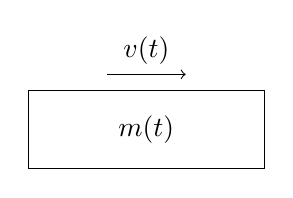
\begin{tikzpicture}
    \draw (0, 0.5) rectangle (3, -0.5);
    \node at (1.5, 0) {$m(t)$};
    \draw [->] (1, 0.7) -- (2, 0.7) node [pos = 0.5, above] {$v(t)$};
  \end{tikzpicture}
\end{center}
At time $t + \delta t$, it ejects exhaust of mass $m(t) - m(t + \delta t)$ with velocity $v(t) - u + O(\delta t)$.
\begin{center}
  \begin{tikzpicture}
    \draw (0, 0.5) rectangle (3, -0.5);
    \node at (1.5, 0) {$m(t)$};
    \draw [->] (1, 0.7) -- (2, 0.7) node [pos = 0.5, above] {$v(t)$};
    \node at (-1, 0) [circ] {$m$};
    \draw [->] (-1.33, 0) -- (-2, 0) node [left] {$v(t) - u$};
  \end{tikzpicture}
\end{center}
The change in total momentum of the system (rocket + exhaust) is
\begin{align*}
  \delta p &= m(t + \delta t)v(t + \delta t) + [m(t) - m(t + \delta t)][v(t) - u(t) + O(\delta t)] - m(t)v(t)\\
  &= (m + \dot{m}\delta t + O(\delta t^2))(v + \dot{v} \delta t + O(\delta t^2)) - \dot{m}\delta t(v - u) + O(\delta t^2) - mv\\
  &= (\dot{m}v + m\dot{v} - \dot{m}v + \dot{m}u)\delta t + O(\delta t^2)\\
  &= (m\dot{v} + \dot{m}u)\delta t + O(\delta t^2).
\end{align*}
Newton's second law gives
\[
  \lim_{\delta \to 0} \frac{\delta p}{\delta t} = F
\]
where $F$ is the external force on the rocket. So we obtain
\begin{prop}[Rocket equation]
  \[
    m\frac{\d v}{\d t} + u\frac{\d m}{\d t} = F.
  \]
\end{prop}
\begin{eg}
  Suppose that we travel in space with $F = 0$. Assume also that $u$ is constant. Then we have
  \[
    m\frac{\d v}{\d t} = -u\frac{\d m}{d t}.
  \]
  So
  \[
    v = v_0 + u \log \left(\frac{m_0}{m(t)}\right),
  \]
  Note that we are expressing things in terms of the mass remaining $m$, not time $t$.

  Note also that the velocity does not depend on the rate at which mass is ejected, only the velocity at which it is ejected. Of course, if we expressed $v$ as a function of time, then the velocity at a specific time \emph{does} depend on the rate at which mass is ejected.
\end{eg}

\begin{eg}
  Consider a falling raindrop of mass $m(t)$, gathering mass from a stationary cloud. In this case, $u = v$. So
  \[
    m\frac{\d v}{\d t} + v\frac{\d m}{\d t} = \frac{\d }{\d t}(mv) = mg,
  \]
  with $v$ measured downwards. To obtain a solution of this, we will need a model to determine the rate at which the raindrop gathers mass.
\end{eg}

\section{Rigid bodies}
This chapter is somewhat similar to the previous chapter. We again have a lot of particles and we study their motion. However, instead of having forces between the individual particles, this time the particles are constrained such that their relative positions are fixed. This corresponds to a solid object that cannot deform. We call these \emph{rigid bodies}.

\begin{defi}[Rigid body]
  A \emph{rigid body} is an extended object, consisting of $N$ particles that are constrained such that the distance between any pair of particles, $|\mathbf{r}_i - \mathbf{r}_j|$, is fixed.
\end{defi}

The possible motions of a rigid body are the continuous isometries of Euclidean space, i.e.\ translations and rotations. However, as we have previously shown, pure translations of rigid bodies are uninteresting --- they simply correspond to the center of mass moving under an external force. Hence we will first study rotations.

Later, we will combine rotational and translational effects and see what happens.

\subsection{Angular velocity}
We'll first consider the cases where there is just one particle, moving in a circle of radius $s$ about the $z$ axis. Its position and velocity vectors are
\begin{align*}
  \mathbf{r} &= (s\cos \theta, s\sin \theta, z)\\
  \dot{\mathbf{r}} &= (-s \dot{\theta}\sin \theta, s\dot{\theta}\cos \theta, 0).
\end{align*}
We can write
\[
  \dot{\mathbf{r}} = \boldsymbol\omega\times \mathbf{r},
\]
where
\[
  \boldsymbol\omega = \dot{\theta}\hat{\mathbf{z}}
\]
is the angular velocity vector.

In general, we write
\[
  \boldsymbol\omega = \dot{\theta} \hat{\mathbf{n}} = \omega\hat{\mathbf{n}},
\]
where $\hat{\mathbf{n}}$ is a unit vector parallel to the rotation axis.

The kinetic energy of this particle is thus
\begin{align*}
  T &= \frac{1}{2}m|\dot{\mathbf{r}}|^2\\
  &= \frac{1}{2}m s^2 \dot{\theta}^2\\
  &= \frac{1}{2}I \omega^2
\end{align*}
where $I = ms^2$ is the \emph{moment of inertia}. This is the counterpart of ``mass'' in rotational motion.
\begin{defi}[Moment of inertia]
  The \emph{moment of inertia} of a particle is
  \[
    I = ms^2 = m|\hat{\mathbf{n}}\times \mathbf{r}|^2,
  \]
  where $s$ is the distance of the particle from the axis of rotation.
\end{defi}
\subsection{Moment of inertia}
In general, consider a rigid body in which all $N$ particles rotate about the same axis with the same angular velocity:
\[
  \dot{\mathbf{r}}_i = \boldsymbol\omega\times \mathbf{r}_i.
\]
This ensures that
\[
  \frac{\d }{\d t}|\mathbf{r}_i - \mathbf{r}_j|^2 = 2(\dot{\mathbf{r}}_i - \dot{\mathbf{r}}_j)\cdot (\mathbf{r}_i - \mathbf{r}_j) = 2\big(\boldsymbol\omega\times (\mathbf{r}_i - \mathbf{r}_j)\big) \cdot (\mathbf{r}_i - \mathbf{r}_j) = 0,
\]
as required for a rigid body.

Similar to what we had above, the rotational kinetic energy is
\[
  T = \frac{1}{2}\sum_{i = 1}^N m_i|\dot{\mathbf{r}_i}|^2 = \frac{1}{2}I\omega^2,
\]
where
\begin{defi}[Moment of inertia]
  The \emph{moment of inertia} of a rigid body about the rotation axis $\hat{\mathbf{n}}$ is
  \[
    I = \sum_{i = 1}^N m_is_i^2 = \sum_{i = 1}^N m_i |\hat{\mathbf{n}}\times \mathbf{r}_i|^2.
  \]
\end{defi}
Again, we define the angular momentum of the system:
\begin{defi}
  The \emph{angular momentum} is
  \[
    \mathbf{L} = \sum_i m_i \mathbf{r}_i \times \dot{\mathbf{r}}_i = \sum_i m_i \mathbf{r}_i \times (\boldsymbol\omega \times \mathbf{r}_i).
  \]
\end{defi}
Note that our definitions for angular motion are analogous to those for linear motion. The moment of inertia $I$ is defined such that $T = \frac{1}{2}I\omega^2$. Ideally, we would want the momentum to be $\mathbf{L} = I\boldsymbol \omega$. However, this not true. In fact, $\mathbf{L}$ need not be parallel to $\boldsymbol\omega$.

What \emph{is} true, is that the component of $\mathbf{L}$ parallel to $\boldsymbol\omega$ is equal to $I\omega$. Write $\boldsymbol\omega = \omega\hat{\mathbf{n}}$. Then we have
\begin{align*}
  \mathbf{L} \cdot \hat{\mathbf{n}} &= \omega \sum_i m_i \hat{\mathbf{n}}\cdot (\mathbf{r}_i \times (\hat{\mathbf{n}} \times \mathbf{r}_i))\\
  &= \omega \sum_i m(\hat{\mathbf{n}}\times \mathbf{r}_i)\cdot (\hat{\mathbf{n}} \times \mathbf{r}_i)\\
  &= I\omega.
\end{align*}
What does $\mathbf{L}$ itself look like? Using vector identities, we have
\[
  \mathbf{L} = \sum_i m_i\big((\mathbf{r}_i\cdot \mathbf{r}_i)\boldsymbol \omega - (\mathbf{r}_i \cdot \boldsymbol\omega)\mathbf{r}_i\big)
\]
Note that this is a linear function of $\boldsymbol\omega$. So we can write
\[
  \mathbf{L} = I\boldsymbol \omega,
\]
where we abuse notation to use $I$ for the \emph{inertia tensor}. This is represented by a symmetric matrix with components
\[
  I_{jk} = \sum_i m_i(|\mathbf{r}_i|^2 \delta_{jk} - (\mathbf{r}_i)_j(\mathbf{r}_i)_k),
\]
where $i$ refers to the index of the particle, and $j, k$ are dummy suffixes.

If the body rotates about a \emph{principal axis}, i.e.\ one of the three orthogonal eigenvectors of $I$, then $\mathbf{L}$ will be parallel to $\boldsymbol\omega$. Usually, the principal axes lie on the axes of rotational symmetry of the body.

\subsection{Calculating the moment of inertia}
For a solid body, we usually want to think of it as a continuous substance with a mass density, instead of individual point particles. So we replace the sum of particles by a volume integral weighted by the mass density $\rho(\mathbf{r})$.

\begin{defi}[Mass, center of mass and moment of inertia]
  The \emph{mass} is
  \[
    M = \int \rho \;\d V.
  \]
  The \emph{center of mass} is
  \[
    \mathbf{R} = \frac{1}{M}\int \rho \mathbf{r}\;\d V
  \]
  The \emph{moment of inertia} is
  \[
    I = \int \rho s^2 \;\d V = \int \rho|\hat{\mathbf{n}}\times \mathbf{r}|^2\;\d V.
  \]
\end{defi}
In theory, we can study inhomogeneous bodies with varying $\rho$, but usually we mainly consider homogeneous ones with constant $\rho$ throughout.

\begin{eg}[Thin circular ring]
  Suppose the ring has mass $M$ and radius $a$, and a rotation axis through the center, perpendicular to the plane of the ring.
  \begin{center}
    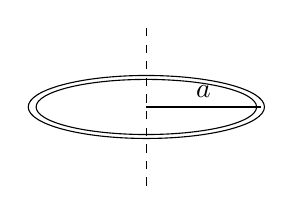
\begin{tikzpicture}
      \draw circle [x radius = 1.5, y radius = 0.4];
      \draw circle [x radius = 1.4, y radius = 0.35];
      \draw (0, 0) -- (1.45, 0) node [pos = 0.5, above] {$a$};
      \draw [dashed] (0, -1) -- (0, 1);
    \end{tikzpicture}
  \end{center}
  Then the moment of inertia is
  \[
    I = Ma^2.
  \]
\end{eg}

\begin{eg}[Thin rod]
  Suppose a rod has mass $M$ and length $\ell$. It rotates through one end, perpendicular to the rod.
  \begin{center}
    \begin{tikzpicture}
      \draw [dashed] (0, -1) -- (0, 1);
      \draw (0, 0.05) rectangle (2, -0.05);
      \node at (1, 0.3) {$\ell$};
    \end{tikzpicture}
  \end{center}
  The mass per unit length is $M/\ell$. So the moment of inertia is
  \[
    I = \int_0 ^\ell \frac{M}{\ell}x^2\;\d x = \frac{1}{3}M\ell^2.
  \]
\end{eg}

\begin{eg}[Thin disc]
  Consider a disc of mass $M$ and radius $a$, with a rotation axis through the center, perpendicular to the plane of the disc.
  \begin{center}
    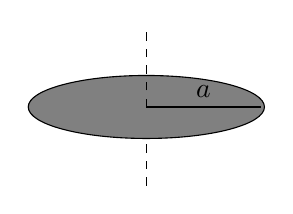
\begin{tikzpicture}
      \draw [fill=gray] circle[x radius = 1.5, y radius = 0.4];
      \draw (0, 0) -- (1.45, 0) node [pos = 0.5, above] {$a$};
      \draw [dashed] (0, -1) -- (0, -0.4);
      \draw [dashed] (0, 0) -- (0, 1);
    \end{tikzpicture}
  \end{center}
  Then
  \begin{align*}
    I &= \int_{0}^{2\pi}\int_0^a \underbrace{\frac{M}{\pi a^2}}_{\text{mass per unit length}} \underbrace{r^2}_{s^2} \underbrace{r\;\d r\;\d \theta}_{\text{area element}}\\
    &= \frac{M}{\pi a^2}\int_0^a r^3\;\d r \int_0^{2\pi}\;\d \theta\\
    &= \frac{M}{\pi a^2}\frac{1}{4}a^4 (2\pi)\\
    &= \frac{1}{2}Ma^2.
  \end{align*}
  Now suppose that the rotation axis is in the plane of the disc instead (also rotating through the center). Then
  \begin{align*}
    I &= \int_{0}^{2\pi}\int_0^a \underbrace{\frac{M}{\pi a^2}}_{\text{mass per unit length}} \underbrace{(r\sin \theta)^2}_{s^2} \underbrace{r\;\d r\;\d \theta}_{\text{area element}}\\
    &= \frac{M}{\pi a^2}\int_0^a r^3\;\d r \int_0^{2\pi}\sin^2 \theta\;\d \theta\\
    &= \frac{M}{\pi a^2}\frac{1}{4}a^4 \pi\\
    &= \frac{1}{4}Ma^2.
  \end{align*}
\end{eg}
\begin{eg}
  Consider a solid sphere with mass $M$, radius $a$, with a rotation axis though the center.
  \begin{center}
    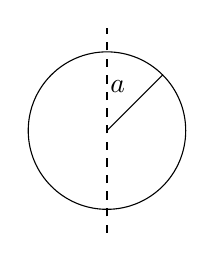
\begin{tikzpicture}
      \draw circle [radius = 1];
      \draw (0, 0) -- (0.707, 0.707) node [pos =0.5, anchor = south east] {$a$};
      \draw [dashed] (0, -1.3) -- (0, 1.3);
    \end{tikzpicture}
  \end{center}
  Using spherical polar coordinates $(r, \theta, \phi)$ based on the rotation axis,
  \begin{align*}
    I &= \int_{0}^{2\pi}\int_0^\pi\int_0^a \underbrace{\frac{M}{\frac{4}{3}\pi a^3}}_{\rho}\underbrace{(r\sin \theta)^2}_{s^2} \underbrace{r^2\sin \theta\;\d r\;\d \theta\;\d \phi}_{\text{volume element}}\\
    &= \frac{M}{\frac{4}{3}\pi a^3}\int_0^a r^4 \;\d r\int_0^\pi (1 - \cos^2)\sin \theta\;\d \theta \int_0^{2\pi}\;\d \phi\\
    &= \frac{M}{\frac{4}{3}\pi a^3}\cdot \frac{1}{5}a^5 \cdot \frac{4}{3}\cdot 2\pi\\
    &= \frac{2}{5}Ma^2.
  \end{align*}
\end{eg}

Usually, finding the moment of inertia involves doing complicated integrals. We will now come up with two theorems that help us find moments of inertia.
\begin{thm}[Perpendicular axis theorem]
  For a two-dimensional object (a lamina), and three perpendicular axes $x, y, z$ through the same spot, with $z$ normal to the plane,
  \[
    I_z = I_x + I_y,
  \]
  where $I_z$ is the moment of inertia about the $z$ axis.
  \begin{center}
    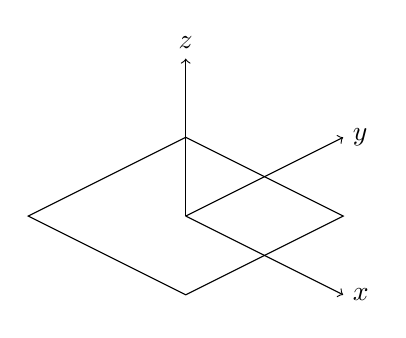
\begin{tikzpicture}
      \draw [->] (0, 0) -- (2, -1) node [right] {$x$};
      \draw [->] (0, 0) -- (2, 1) node [right] {$y$};
      \draw [->] (0, 0) -- (0, 2) node [above] {$z$};
      \draw (-2, 0) -- (0, -1) -- (2, 0) -- (0, 1) -- cycle;
    \end{tikzpicture}
  \end{center}
\end{thm}
Note that this does \emph{not} apply to 3D objects! For example, in a sphere, $I_x = I_y = I_z$.

\begin{proof}
  Let $\rho$ be the mass per unit volume. Then
  \begin{align*}
    I_x &= \int \rho y^2 \;\d A\\
    I_y &= \int \rho x^2 \;\d A\\
    I_z &= \int \rho (x^2 + y^2)\;\d A = I_x + I_y.\qedhere
  \end{align*}
\end{proof}

\begin{eg}
  For a disc, $I_x = I_y$ by symmetry. So $I_z = 2 I_x$.
\end{eg}

\begin{thm}[Parallel axis theorem]
  If a rigid body of mass $M$ has moment of inertia $I^C$ about an axis passing through the center of mass, then its moment of inertia about a parallel axis a distance $d$ away is
  \[
    I = I^C + Md^2.
  \]
  \begin{center}
    \begin{tikzpicture}
      \draw plot [smooth cycle] coordinates{(0, 0) (1, -2) (3, -1) (4, 0) (4, 1) (2, 1) (1, 3)};
      \node [circ] at (2, 0) {};
      \node at (2, 0) [left] {CM};
      \draw [dashed] (2, -2.5) -- (2, 3);
      \draw [dashed] (3, -2.5) -- (3, 3);
      \draw [->] (2, 0) -- (3, 0);
      \draw [->] (3, 0) -- (2, 0) node [pos = 0.5, above] {$d$};
    \end{tikzpicture}
  \end{center}
\end{thm}

\begin{proof}
  With a convenient choice of Cartesian coordinates such that the center of mass is at the origin and the two rotation axes are $x = y =0$ and $x = d, y = 0$,
  \[
    I^C = \int \rho (x^2 + y^2) \;\d V,
  \]
  and
  \[
    \int \rho \mathbf{r}\;\d V = \mathbf{0}.
  \]
  So
  \begin{align*}
    I &= \int \rho((x - d)^2 + y^2)\;\d V\\
    &=\int \rho (x^2 + y^2)\;\d V - 2d\int \rho x\;\d V + \int d^2 \rho\;\d V\\
    &= I^c + 0 + Md^2\\
    &= I^c + Md^2.\qedhere
  \end{align*}
\end{proof}

\begin{eg}
  Take a disc of mass $M$ and radius $a$, and rotation axis through a point on the circumference, perpendicular to the plane of the disc. Then
  \begin{center}
    \begin{tikzpicture}
      \draw [fill=gray] circle [x radius = 2, y radius = 0.6];
      \node [circ] {};
      \draw (0, 0) -- (1.03, 0.5) node [pos = 0.5, anchor = south east] {$a$};
      \draw [dashed] (2, -1) -- (2, 1);
    \end{tikzpicture}
  \end{center}
  \[
    I = I^c + Ma^2 = \frac{1}{2}Ma^2 + Ma^2 = \frac{3}{2}Ma^2.
  \]
\end{eg}

\subsection{Motion of a rigid body}
The general motion of a rigid body can be described as a translation of its centre of mass, following a trajectory $\mathbf{R}(t)$, together with a rotation about an axis through the center of mass. As before, we write
\[
  \mathbf{r}_i = \mathbf{R} + \mathbf{r}_i^c.
\]
Then
\[
  \dot{\mathbf{r}}_i = \dot{\mathbf{R}} + \dot{\mathbf{r}}_i^c.
\]
Using this, we can break down the velocity and kinetic energy into translational and rotational parts.

If the body rotates with angular velocity $\boldsymbol\omega$ about the center of mass, then
\[
  \dot{\mathbf{r}}_i^c = \boldsymbol\omega \times \mathbf{r}_i^c.
\]
Since $\mathbf{r}_i^c = \mathbf{r}_i - \mathbf{R}$, we have
\[
  \dot{\mathbf{r}_i} = \dot{\mathbf{R}} + \boldsymbol \omega \times \mathbf{r}_i^c = \dot{\mathbf{R}} + \boldsymbol\omega\times (\mathbf{r}_i - \mathbf{R}).
\]
On the other hand, the kinetic energy, as calculated in previous lectures, is
\begin{align*}
  T &= \frac{1}{2}M|\dot{\mathbf{R}}|^2 + \frac{1}{2}\sum_i m_i |\dot{\mathbf{r}}_i^c|^2\\
  &= \underbrace{\frac{1}{2}M|\dot{\mathbf{R}}|^2}_{\text{translational KE}} + \underbrace{\frac{1}{2}I^c\omega^2}_{\text{rotational KE}}.
\end{align*}
Sometimes we do not want to use the center of mass as the center. For example, if an item is held at the edge and spun around, we'd like to study the motion about the point at which the item is held, and not the center of mass.

So consider any point $Q$, with position vector $\mathbf{Q}(t)$ that is not the center of mass but moves with the rigid body, i.e.
\[
  \dot{\mathbf{Q}} = \dot{\mathbf{R}} + \boldsymbol\omega\times (\mathbf{Q} - \mathbf{R}).
\]
Usually this is a point inside the object itself, but we do not assume that in our calculation.

Then we can write
\begin{align*}
  \dot{\mathbf{r}}_i &= \dot{\mathbf{R}} + \boldsymbol\omega\times (\mathbf{r}_i - \mathbf{R})\\
  &= \dot{\mathbf{Q}} - \boldsymbol\omega\times (\mathbf{Q} - \mathbf{R}) + \boldsymbol\omega \times (\mathbf{r}_i - \mathbf{R})\\
  &= \dot{\mathbf{Q}} + \boldsymbol\omega\times (\mathbf{r}_i - \mathbf{Q}).
\end{align*}
Therefore the motion can be considered as a translation of $Q$ (with \emph{different} velocity than the center of mass), together with rotation about $Q$ (with the \emph{same} angular velocity $\boldsymbol\omega$).

\subsubsection*{Equations of motion}
As shown previously, the linear and angular momenta evolve according to
\begin{align*}
  \dot{\mathbf{P}} &= \mathbf{F}\quad \text{(total external force)}\\
  \dot{\mathbf{L}} &= \mathbf{G}\quad \text{(total external torque)}
\end{align*}
These two equations determine the translational and rotational motion of a rigid body.

$\mathbf{L}$ and $\mathbf{G}$ depend on the choice of origin, which could be any point that is fixed in an inertial frame. More surprisingly, it can also be applied to the center of mass, even if this is accelerated:
If
\[
  m_i \ddot{\mathbf{r}}_i = \mathbf{F}_i,
\]
then
\[
  m_i \ddot{\mathbf{r}}_i^c = \mathbf{F}_i + m_i \ddot{\mathbf{R}}.
\]
So there is a fictitious force $m_i \ddot{\mathbf{R}}$ in the center-of-mass frame. But the total torque of the fictitious forces about the center of mass is
\[
  \sum_i \mathbf{r}_i^c \times \left(-m_i \ddot{\mathbf{R}}\right) = -\left(\sum m_i \mathbf{r}_i^c\right) \times \ddot{\mathbf{R}} = \mathbf{0}\times \dot{\mathbf{R}} = 0.
\]
So we can still apply the above two equations.

In summary, the laws of motion apply in any inertial frame, or the center of mass (possibly non-inertial) frame.

\subsubsection*{Motion in a uniform gravitational field}
In a uniform gravitational field $\mathbf{g}$, the total gravitational force and torque are the same as those that would act on a single particle of mass $M$ located at the center of mass (which is also the \emph{center of gravity}):
\[
  \mathbf{F} = \sum_i \mathbf{F}_i^{\mathrm{ext}} = \sum_i m_i \mathbf{g} = M\mathbf{g},
\]
and
\[
  \mathbf{G} = \sum_i \mathbf{G}_i^{\mathrm{ext}} = \sum_i \mathbf{r}_i \times (m_i \mathbf{g}) = \sum m_i \mathbf{r}_i \times \mathbf{g} = M\mathbf{R}\times \mathbf{g}.
\]
In particular, the gravitational torque about the center of mass vanishes: $\mathbf{G}^c = \mathbf{0}$.

We obtain a similar result for gravitational potential energy.

The gravitational potential in a uniform $\mathbf{g}$ is
\[
  \Phi_g = -\mathbf{r}\cdot \mathbf{g}.
\]
(since $\mathbf{g} = -\nabla \Phi_g$ by definition)

So
\begin{align*}
  V^{\mathrm{ext}} &= \sum_i V_i^{\mathrm{ext}}\\
  &= \sum_i m_i (- \mathbf{r}_i \cdot \mathbf{g})\\
  &= M (-\mathbf{R}\cdot \mathbf{g}).
\end{align*}

\begin{eg}[Thrown stick]
  Suppose we throw a symmetrical stick. So the center of mass is the actual center. Then the center of the stick moves in a parabola. Meanwhile, the stick rotates with constant angular velocity about its center due to the absence of torque.
\end{eg}

\begin{eg}
  Swinging bar.
  \begin{center}
    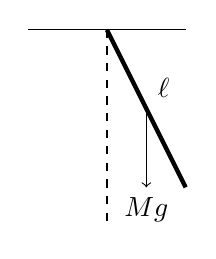
\begin{tikzpicture}
      \draw (-1, 0) -- (1, 0);
      \draw [ultra thick] (0, 0) -- (1, -2) node [anchor = south west, pos = 0.5] {$\ell$};
      \draw [dashed] (0, 0) -- (0, -2.5);
      \draw [->] (0.5, -1) -- (0.5, -2) node [below] {$Mg$};
    \end{tikzpicture}
  \end{center}
  This is an example of a \emph{compound pendulum}.

  Consider the bar to be rotating about the pivot (and not translating). Its angular momentum is $L = I\dot{\theta}$ with $I = \frac{1}{3}M\ell^2$. The gravitational torque about the pivot is
  \[
    G = - Mg\frac{\ell}{2} \sin \theta.
  \]
  The equation of motion is
  \[
    \dot{L} = G.
  \]
  So
  \[
    I\ddot{\theta} = -Mg \frac{\ell}{2}\sin \theta,
  \]
  or
  \[
    \ddot{\theta} = -\frac{3g}{2\ell} \sin \theta.
  \]
  which is exactly equivalent to a simple pendulum of length $2\ell/3$, with angular frequency $\sqrt{\frac{3g}{2\ell}}$.

  This can also be obtained from an energy argument:
  \[
    E = T + V = \frac{1}{2}I\dot{\theta}^2 - Mg\frac{\ell}{2}\cos\theta.
  \]
  We differentiate to obtain
  \[
    \frac{\d E}{\d t} = \dot{\theta}(I\ddot{\theta} + Mg \frac{\ell}{2}\sin \theta) = 0.
  \]
  So
  \[
    I\ddot{\theta} = -Mg \frac{\ell}{2}\sin \theta.
  \]
\end{eg}

\subsubsection*{Sliding versus rolling}
Consider a cylinder or sphere of radius $a$, moving along a stationary horizontal surface.
\begin{center}
  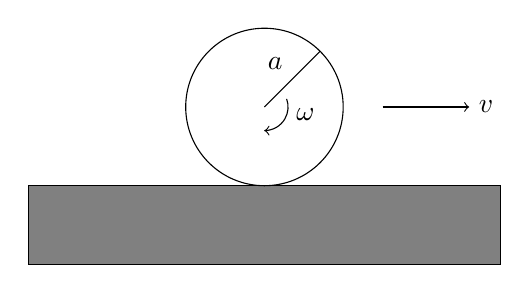
\begin{tikzpicture}
    \draw [fill = gray] (-3, 0) rectangle (3, -1);
    \draw (0, 1) circle [radius=1];
    \draw (0, 1) -- (0.707, 1.707) node [pos=0.5, anchor = south east] {$a$};
    \draw [->] (1.5, 1) -- (2.6, 1) node [right] {$v$};
    \draw (0, 0.7) arc (270:380:0.3) node [anchor = north west] {$\omega$};
    \draw [->] (0.01, 0.7) -- (0, 0.7);
  \end{tikzpicture}
\end{center}
In general, the motion consists of a translation of the center of mass (with velocity $v$) plus a rotation about the center of mass (with angular velocity $\omega$).

The horizontal velocity at the point of contact is
\[
  v_{\text{slip}} = v - a\omega.
\]
For a pure sliding motion, $v \not = 0$ and $\omega = 0$, in which case $v - a\omega \not = 0$: the point of contact moves relative to the surface and kinetic friction may occur.

For a pure rolling motion, $v\not = 0$ and $\omega \not = 0$ such that $v - a\omega = 0$: the point of contact is stationary. This is the no-slip condition.

The rolling body can alternatively be considered to be rotating instantaneously about the point of contact (with angular velocity $\omega$) and not translating.

\begin{eg}[Rolling down hill]\leavevmode
  \begin{center}
    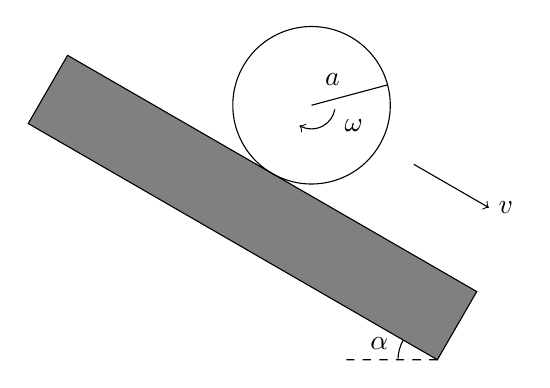
\begin{tikzpicture}[rotate=-30]
      \draw [fill = gray] (-3, 0) rectangle (3, -1);
      \draw (0, 1) circle [radius=1];
      \draw (0, 1) -- (0.707, 1.707) node [pos=0.5, anchor = south east] {$a$};
      \draw [->] (1.5, 1) -- (2.6, 1) node [right] {$v$};
      \draw (0, 0.7) arc (270:380:0.3) node [anchor = north west] {$\omega$};
      \draw [->] (0.01, 0.7) -- (0, 0.7);
      \draw [dashed] (3, -1) -- (2, -1.577);
      \draw (2.5, -1) arc (180:210:0.5) node [anchor = south east] {$\alpha$};
    \end{tikzpicture}
  \end{center}
  Consider a cylinder or sphere of mass $M$ and radius $a$ rolling down a rough plane inclined at angle $\alpha$. The no-slip (rolling) condition is
  \[
    v - a\omega = 0 .
  \]
  The kinetic energy is
  \[
    T = \frac{1}{2}Mv^2 + \frac{1}{2}I\omega^2 = \frac{1}{2}\left(M + \frac{I}{a^2}\right)v^2.
  \]
  The total energy is
  \[
    E = \frac{1}{2}\left(M + \frac{I}{a^2}\right) \dot{x}^2 - Mgx\sin \alpha,
  \]
  where $x$ is the distance down slope. While there is a frictional force, the instantaneous velocity is $0$, and no work is done. So energy is conserved, and we have
  \[
    \frac{\d E}{\d t} = \dot{x}\left(\left(M + \frac{I}{a^2}\right)\ddot{x} - Mg\sin \alpha\right) = 0.
  \]
  So
  \[
    \left(M + \frac{I}{a^2}\right)\ddot{x} = Mg\sin \alpha.
  \]
  For example, if we have a uniform solid cylinder,
  \[
    I = \frac{1}{2}Ma^2\quad\text{(as for a disc)}
  \]
  and so
  \[
    \ddot{x} = \frac{2}{3}g\sin \alpha.
  \]
  For a thin cylindrical shell,
  \[
    I = Ma^2.
  \]
  So
  \[
    \ddot{x} = \frac{1}{2}g\sin \alpha.
  \]
  Alternatively, we may do it in terms of forces and torques,
  \begin{center}
    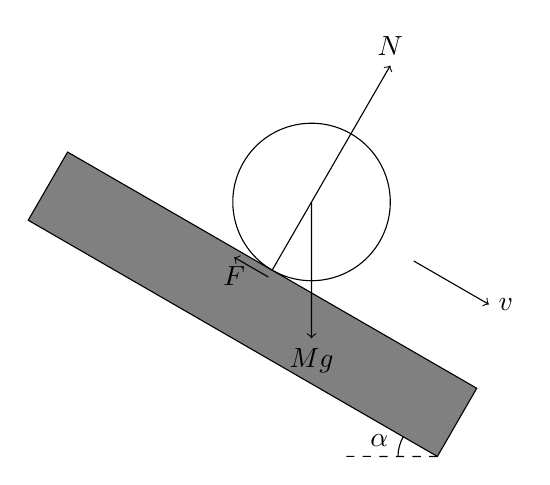
\begin{tikzpicture}[rotate=-30]
      \draw [fill = gray] (-3, 0) rectangle (3, -1);
      \draw (0, 1) circle [radius=1];
      \draw [->] (1.5, 1) -- (2.6, 1) node [right] {$v$};
      \draw [dashed] (3, -1) -- (2, -1.577);
      \draw (2.5, -1) arc (180:210:0.5) node [anchor = south east] {$\alpha$};
      \draw [->] (0, 0) -- (0, 3) node [above] {$N$};
      \draw [->] (0, -0.1) -- (-0.5, -0.1) node [below] {$F$};
      \draw [->] (0, 1) -- (0.866, -0.5) node [below] {$Mg$};
    \end{tikzpicture}
  \end{center}
  The equations of motion are
  \[
    M\dot{v} = Mg\sin \alpha - F
  \]
  and
  \[
    I\dot \omega = aF.
  \]
  While rolling,
  \[
    \dot{v} - a\dot\omega = 0.
  \]
  So
  \[
    M\dot{v} = Mg\sin \alpha - \frac{I}{a^2}\dot{v},
  \]
  leading to the same result.

  Note that even though there is a frictional force, it does no work, since $v_{\mathrm{slip}} = 0$. So energy is still conserved.
\end{eg}

\begin{eg}[Snooker ball]\leavevmode
  \begin{center}
    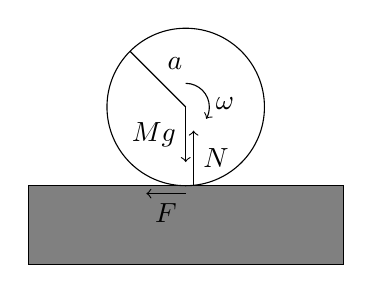
\begin{tikzpicture}
      \draw [fill=gray] (-2, 0) rectangle (2, -1);
      \draw (0, 1) circle [radius=1];
      \draw (0, 1) -- (-0.707, 1.707) node [pos = 0.5, anchor = south west] {$a$};
      \draw [->] (0.1, 0) -- (0.1, 0.7) node [pos = 0.5, right] {$N$};
      \draw [->] (0, 1) -- (0, 0.3) node [pos = 0.5, left] {$Mg$};
      \draw [->] (0, -0.1) -- (-0.5, -0.1) node [pos = 0.5, below] {$F$};
      \draw [->] (0, 1.3) arc (90:-30:0.3) node [anchor = south west] {$\omega$};
    \end{tikzpicture}
  \end{center}
  It is struck centrally so as to initiate translation, but not rotation. Sliding occurs initially. Intuitively, we think it will start to roll, and we'll see that's the case.

  The constant frictional force is
  \[
    F = \mu_k N = \mu_k Mg,
  \]
  which applies while $v - a\omega > 0$.

  The moment of inertia about the center of mass is
  \[
    I = \frac{2}{5}Ma^2.
  \]
  The equations of motion are
  \begin{align*}
    M\dot{v} &= -F\\
    I\dot\omega &= aF
  \end{align*}
  Initially, $v = v_0$ and $\omega = 0$. Then the solution is
  \begin{align*}
    v &= v_0 - \mu_k gt\\
    \omega &= \frac{5}{2} \frac{\mu_k g}{a}t
  \end{align*}
  as long as $v - a \omega > 0$. The slip velocity is
  \[
    v_{\mathrm{slip}} = v - a\omega = v_0 - \frac{7}{2}\mu_k gt = v_0 \left(1 - \frac{t}{t_\mathrm{roll}}\right),
  \]
  where
  \[
    t_{\mathrm{roll}} = \frac{2v_0}{7\mu_k g}.
  \]
  This is valid up till $t = t_{\mathrm{roll}}$. Then the slip velocity is 0, rolling begins and friction ceases.

  At this point, $v = a\omega = \frac{5}{7}v_0$. The energy is then $\frac{5}{14}Mv_0^2 < \frac{1}{2}Mv_0^2$. So energy is lost to friction.
\end{eg}
\section{Special relativity}
When particles move Extremely Fast\textsuperscript{TM}, Newtonian Dynamics becomes inaccurate and is replaced by Einstein's Special Theory of Relativity (1905).

Its effects are noticeable only when particles approach to the speed of light,
\[
  c = \SI{299792458}{\meter\per\second} \approx \SI{3e8}{\meter\per\second}
\]
This is \emph{really fast}.

The Special Theory of Relativity rests on the following postulate:
\begin{center}
  \emph{The laws of physics are the same in all inertial frames}
\end{center}
This is the principle of relativity familiar to Galileo. Galilean relativity mentioned in the first chapter satisfies this postulate for dynamics. People then thought that Galilean relativity is what the world obeys. However, it turns out that there is a whole family of solutions that satisfy the postulate (for dynamics), and Galilean relativity is just one of them.

This is not a problem (yet), since Galilean relativity seems so intuitive, and we might as well take it to be the true one. However, it turns out that solving Maxwell's equations of electromagnetism gives an explicit value of the speed of light, $c$. This is independent of the frame of reference. So the speed of light must be the same in every inertial frame.

This is not compatible with Galilean relativity.

Consider the two inertial frames $S$ and $S'$, moving with relative velocity $v$. Then if light has velocity $c$ in $S$, then Galilean relativity predicts it has velocity $c - v$ in $S'$, which is wrong.

Therefore, we need to find a different solution to the principle of relativity that preserves the speed of light.

\subsection{The Lorentz transformation}
Consider again inertial frames $S$ and $S'$ whose origins coincide at $t = t' = 0$. For now, neglect the $y$ and $z$ directions, and consider the relationship between $(x, t)$ and $(x', t')$. The general form is
\[
  x' = f(x, t),\quad t' = g(x, t),
\]
for some functions $f$ and $g$. This is not very helpful.

In any inertial frame, a free particle moves with constant velocity. So straight lines in $(x, t)$ must map into straight lines in $(x', t')$. Therefore the relationship must be linear.

Given that the origins of $S$ and $S'$ coincide at $t = t' = 0$, and $S'$ moves with velocity $v$ relative to $S$, we know that the line $x = vt$ must map into $x'= 0$.

Combining these two information, the transformation must be of the form
\[
  x' = \gamma(x - vt),\tag{1}
\]
for some factor $\gamma$ that may depend on $|v|$ (\emph{not} $v$ itself. We can use symmetry arguments to show that $\gamma$ should take the same value for velocities $v$ and $-v$).

Note that Galilean transformation is compatible with this -- just take $\gamma$ to be always $1$.

Now reverse the roles of the frames. From the perspective $S'$, $S$ moves with velocity $-v$. A similar argument leads to
\[
  x = \gamma(x' + vt'),\tag{2}
\]
with the same factor $\gamma$, since $\gamma$ only depends on $|v|$. Now consider a light ray (or photon) passing through the origin $x = x' = 0$ at $t = t' = 0$. Its trajectory in $S$ is
\[
  x = ct.
\]
We want a $\gamma$ such that the trajectory in $S'$ is
\[
  x' = ct'
\]
as well, so that the speed of light is the same in each frame. Substitute these into (1) and (2)
\begin{align*}
  ct' &= \gamma(c - v)t\\
  ct &= \gamma(c + v)t'
\end{align*}
Multiply the two equations together and divide by $tt'$ to obtain
\[
  c^2 = \gamma^2(c^2 - v^2).
\]
So
\[
  \gamma = \sqrt{\frac{c^2}{c^2 - v^2}} = \frac{1}{\sqrt{1 - (v/c)^2}}.
\]
\begin{defi}[Lorentz factor]
  The \emph{Lorentz factor} is
  \[
    \gamma = \frac{1}{\sqrt{1 - (v/c)^2}}.
  \]
\end{defi}
Note that
\begin{itemize}
  \item $\gamma \geq 1$ and is an increasing function of $|v|$.
  \item When $v \ll c$, then $\gamma \approx 1$, and we recover the Galilean transformation.
  \item When $|v|\to c$, then $\gamma\to \infty$.
  \item If $|v| \geq c$, then $\gamma$ is imaginary, which is physically impossible (or at least \emph{weird}).
  \item If we take $c\to \infty$, then $\gamma = 1$. So Galilean transformation is the transformation we will have if light is infinitely fast. Alternatively, in the world of Special Relativity, the speed of light is ``infinitely fast''.
\end{itemize}
\begin{center}
  \begin{tikzpicture}[xscale=3, yscale=0.2]
    \draw [->] (0, 0) -- (1.1, 0) node [right] {$\frac{v}{c}$};
    \draw [->] (0, 0) -- (0, 15) node [above] {$\gamma$};
    \draw [domain=0:0.997, samples=100] plot (\x, {1 / sqrt(1 - \x * \x)});
    \draw [dashed] (1, 15) -- (1, 0) node [below] {$1$};
  \end{tikzpicture}
\end{center}
For the sense of scale, we have the following values of $\gamma$ at different speeds:
\begin{itemize}
  \item $\gamma = 2$ when $v = 0.866c$.
  \item $\gamma = 10$ when $v = 0.9949$.
  \item $\gamma = 20$ when $v = 0.999c$.
\end{itemize}

We still have to solve for the relation between $t$ and $t'$. Eliminate $x$ between (1) and (2) to obtain
\[
  x = \gamma(\gamma(x - vt) + vt').
\]
So
\[
  t' = \gamma t - (1 - \gamma^{-2})\frac{\gamma x}{v} = \gamma\left(t - \frac{v}{c^2}x\right).
\]
So we have
\begin{law}[Principle of Special Relativity]
  Let $S$ and $S'$ be inertial frames, moving at the relative velocity of $v$. Then
  \begin{align*}
    x' &= \gamma(x - vt)\\
    t' &= \gamma\left(t - \frac{v}{c^2}x\right),
  \end{align*}
  where
  \[
    \gamma = \frac{1}{\sqrt{1 - (v/c)^2}}.
  \]
  This is the \emph{Lorentz transformations} in the standard configuration (in one spatial dimension).
\end{law}
The above is the form the Lorentz transformation is usually written, and is convenient for actual calculations. However, this lacks symmetry between space and time. To display the symmetry, one approach is to use units such that $c = 1$. Then we have
\begin{align*}
  x' &= \gamma(x - vt),\\
  t' &= \gamma(t - vx).
\end{align*}
Alternatively, if we want to keep our $c$'s, instead of comparing $x$ and $t$, which have different units, we can compare $x$ and $ct$. Then we have
\begin{align*}
  x' &= \gamma\left(x - \frac{v}{c}(ct)\right),\\
  ct' &= \gamma\left(ct - \frac{v}{c}x\right).
\end{align*}
Symmetries aside, to express $x, t$ in terms of $x', t'$, we can invert this linear mapping to find (after some algebra)
\begin{align*}
  x &= \gamma(x' + vt')\\
  t &= \gamma\left(t' + \frac{v}{c^2}x'\right)
\end{align*}
Directions perpendicular to the relative motion of the frames are unaffected:
\begin{align*}
  y' &= y\\
  z' &= z
\end{align*}
Now we check that the speed of light is really invariant:

For a light ray travelling in the $x$ direction in $S$:
\[
  x = ct,\quad y = 0,\quad z = 0.
\]
In $S'$, we have
\[
  \frac{x'}{t'} = \frac{\gamma(x - vt)}{\gamma(t - vx/c^2)} = \frac{(c - v)t}{(1 - v/c)t} = c,
\]
as required.

For a light ray travelling in the $Y$ direction in $S$,
\[
  x = 0,\quad y = ct,\quad z = 0.
\]
In $S'$,
\[
  \frac{x'}{t'} = \frac{\gamma(x - vt)}{\gamma(t - vx/c^2)} = -v,
\]
and
\[
  \frac{y'}{t'} = \frac{y}{\gamma(t - vx/c^2} = \frac{c}{\gamma},
\]
and
\[
  z' = 0.
\]
So the speed of light is
\[
  \frac{\sqrt{x'^2 + y'^2}}{t'} = \sqrt{v^2 + \gamma^{-2}c^2} = c,
\]
as required.

More generally, the Lorentz transformation implies
\begin{align*}
  c^2t'^2 - r'^2 &= c^2t'^2 - x'^2 - y'^2 - z'^2\\
  &= c^2 \gamma^2\left(t - \frac{v}{c^2}x\right)^2 - \gamma^2(x - vt)^2 - y^2 - z^2\\
  &= \gamma^2\left(1 - \frac{v^2}{c^2}\right)(c^2t^2 - x^2) - y^2 - z^2\\
  &= c^2t^2 - x^2 - y^2 - z^2\\
  &= c^2t^2 - r^2.
\end{align*}
We say that the quantity $c^2t^2 - x^2 - y^2 - z^2$ is \emph{Lorentz-invariant}.

So if $\frac{r}{t} = c$, then $\frac{r'}{t'} = c$ also.

\subsection{Spacetime diagrams}
It is often helpful to plot out what is happening on a diagram. We plot them on a graph, where the position $x$ is on the horizontal axis and the time $ct$ is on the vertical axis. We use $ct$ instead of $t$ so that the dimensions make sense.
\begin{center}
  \begin{tikzpicture}[yscale=1.3]
    \draw [->] (0, 0) -- (3, 0) node [right] {$x$};
    \draw [->] (0, 0) -- (0, 2.3) node [above] {$ct$};
    \draw (0.7, 0.3) .. controls (0.7, 0.8) and (2, 1.3) .. (2, 1.8) node [right] {world line};

    \node [circ] at (1.35, 1.05) {};
    \node at (1.35, 1.05) [anchor = north west] {$P$};
  \end{tikzpicture}
\end{center}
\begin{defi}[Spacetime]
  The union of space and time in special relativity is called \emph{Minkowski spacetime}. Each point $P$ represents an \emph{event}, labelled by coordinates $(ct, x)$ (note the order!).

  A particle traces out a \emph{world line} in spacetime, which is straight if the particle moves uniformly.

  Light rays moving in the $x$ direction have world lines inclined at $45^\circ$.
  \begin{center}
    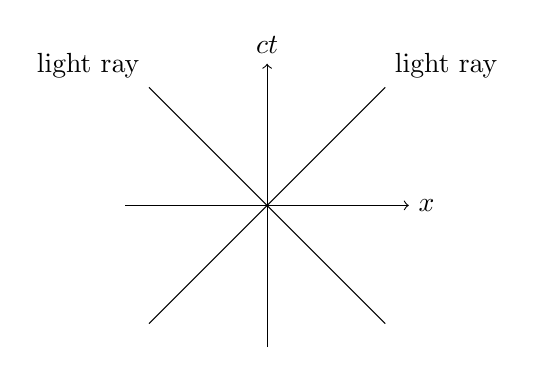
\begin{tikzpicture}[scale=0.6]
      \draw [->] (-3, 0) -- (3, 0) node [right] {$x$};
      \draw [->] (0, -3) -- (0, 3) node [above] {$ct$};
      \draw (-2.5, -2.5) -- (2.5, 2.5) node [anchor = south west] {light ray};
      \draw (2.5, -2.5) -- (-2.5, 2.5) node [anchor = south east] {light ray};
    \end{tikzpicture}
  \end{center}
\end{defi}

We can also draw the axes of $S'$, moving in the $x$ direction at velocity $v$ relative to $S$. The $ct'$ axis corresponds to $x' = 0$, i.e.\ $x = vt$. The $x'$ axis corresponds to $t' = 0$, i.e.\ $t = vx/c^2$.
\begin{center}
  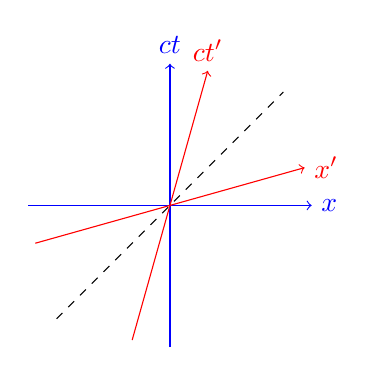
\begin{tikzpicture}[scale=0.6]
    \draw [->, blue] (-3, 0) -- (3, 0) node [right] {$x$};
    \draw [->, blue] (0, -3) -- (0, 3) node [above] {$ct$};
    \draw [->, red] (-2.85, -0.8) -- (2.85, 0.8) node [right] {$x'$};
    \draw [->, red] (-0.8, -2.85) -- (0.8, 2.85) node [above] {$ct'$};
    \draw [dashed] (-2.4, -2.4) -- (2.4, 2.4);
  \end{tikzpicture}
\end{center}
Note that the $x'$ and $ct'$ axes are \emph{not} orthogonal, but are symmetrical about the diagonal (dashed line). So they agree on where the world line of a light ray should lie on.
\subsection{Relativistic physics}
Now we can look at all sorts of relativistic weirdness!
\subsubsection*{Simultaneity}
The first relativistic weirdness is that different frames disagree on whether two evens are simultaneous
\begin{defi}[Simultaneous events]
  We say two events $P_1$ and $P_2$ are simultaneous in the frame $S$ if $t_1 = t_2$.
\end{defi}
They are represented in the following spacetime diagram by horizontal dashed lines.

However, events that are simultaneous in $S'$ have equal values of $t'$, and so lie on lines
\[
  ct - \frac{v}{c}x = \text{constant}.
\]
\begin{center}
  \begin{tikzpicture}[scale=0.6]
    \draw [->, blue] (-3, 0) -- (3, 0) node [right] {$x$};
    \draw [->, blue] (0, -3) -- (0, 3) node [above] {$ct$};
    \draw [dashed, blue] (-3, 1) -- (3, 1);
    \draw [dashed, blue] (-3, 2) -- (3, 2);
    \node [circ] at (-1.5, 2) {};
    \node [circ] at (1.5, 2) {};
    \node at (-1.5, 2) [below] {$P_1$};
    \node at (1.5, 2) [below] {$P_2$};
    \draw [->, red] (-2.85, -0.8) -- (2.85, 0.8) node [right] {$x'$};
    \draw [dashed, red] (-2.85, 0.2) -- (2.85, 1.8);
    \draw [dashed, red] (-2.85, 1.2) -- (2.85, 2.8);
    \draw [->, red] (-0.8, -2.85) -- (0.8, 2.85) node [above] {$ct'$};
  \end{tikzpicture}
\end{center}
The lines of simultaneity of $S'$ and those of $S$ are different, and events simultaneous in $S$ need not be simultaneous in $S'$. So simultaneity is relative. $S$ thinks $P_1$ and $P_2$ happened at the same time, while $S'$ thinks $P_2$ happens first.

Note that this is genuine disagreement. It is not due to effects like, it takes time for the light conveying the information to different observers. Our account above already takes that into account (since the whole discussion does not involve specific observers).

\subsubsection*{Causality}
Although different people may disagree on the temporal order of events, the consistent ordering of cause and effect can be ensured.

Since things can only travel at at most the speed of light, $P$ cannot affect $R$ if $R$ happens a millisecond after $P$ but is at millions of galaxies away. We can draw a \emph{light cone} that denotes the regions in which things can be influenced by $P$. These are the regions of space-time light (or any other particle) can possibly travel to. $P$ can only influence events within its \emph{future light cone}, and \emph{be influenced} by events within its \emph{past light cone}.
\begin{center}
  \begin{tikzpicture}
    \draw [fill=white!60!yellow] (0.5, 0) -- (2, 1.5) -- (3.5, 0);
    \draw [fill=red!50!yellow] (0.5, 3) -- (2, 1.5) -- (3.5, 3);
    \draw (0, 0) -- (4, 0) node [right] {$x$};
    \draw (0, 0) -- (0, 3.5) node [above] {$ct$};
    \node [circ] at (2, 1.5) {};
    \node at (2, 1.5) [left] {$P$};
    \node [circ] at (2, 2.5){};
    \node at (2, 2.5) [left] {$Q$};
    \node [circ] at (3, 2) {};
    \node at (3, 2) [right] {$R$};
  \end{tikzpicture}
\end{center}
All observers agree that $Q$ occurs after $P$. Different observers may disagree on the temporal ordering of $P$ and $R$. However, since nothing can travel faster than light, $P$ and $R$ cannot influence each other. Since everyone agrees on how fast light travels, they also agree on the light cones, and hence causality. So philosophers are happy.

\subsubsection*{Time dilation}
Suppose we have a clock that is stationary in $S'$ (which travels at constant velocity $v$ with respect to inertial frame $S$) ticks at constant intervals $\Delta t'$. What is the interval between ticks in $S$?

Lorentz transformation gives
\[
  t = \gamma\left(t' + \frac{v}{c^2}x'\right).
\]
Since $x' =$ constant for the clock, we have
\[
  \Delta t = \gamma \Delta t' > \Delta t'.
\]
So the interval measured in $S$ is greater! So moving clocks run slowly.

A non-mathematical explanation comes from Feynman (not lectured): Suppose we have a very simple clock: We send a light beam towards a mirror, and wait for it to reflect back. When the clock detects the reflected light, it ticks, and then sends the next light beam.

Then the interval between two ticks is the distance $2d$ divided by the speed of light.
\begin{center}
  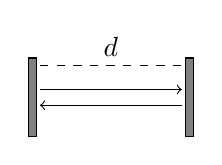
\begin{tikzpicture}
    \draw [fill=gray] (-0.05, -0.5) rectangle (0.05, 0.5);
    \draw [fill=gray] (1.95, -0.5) rectangle (2.05, 0.5);
    \draw [dashed] (0.1, 0.4) -- (1.9, 0.4) node [pos=0.5, above] {$d$};
    \draw [->] (0.1, 0.1) -- (1.9, 0.1);
    \draw [->] (1.9, -0.1) -- (0.1, -0.1);
  \end{tikzpicture}
\end{center}
From the point of view of an observer moving downwards, by the time light reaches the right mirror, it would have moved down a bit. So $S$ sees
\begin{center}
  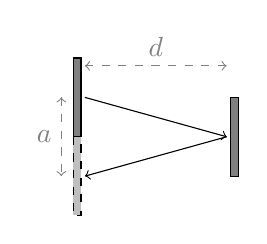
\begin{tikzpicture}
    \draw [fill=gray] (-0.05, -0.5) rectangle (0.05, 0.5);
    \draw [fill=gray] (1.95, -1) rectangle (2.05, 0);
    \draw [->] (0.1, 0) -- (1.9, -0.5);
    \draw [->] (1.9, -0.5) -- (0.1, -1);
    \draw [fill=gray!50!white, dashed] (-0.05, -0.5) rectangle (0.05, -1.5);
    \draw [gray, dashed, ->] (0.1, 0.4) -- (1.9, 0.4) node [pos=0.5, above] {$d$};
    \draw [gray, ->] (0.101, 0.4) -- (0.1, 0.4);
    \draw [gray, ->, dashed] (-0.2, 0) -- (-0.2, -1) node [pos = 0.5, left] {$a$};
    \draw [gray, ->] (-0.2, -0.01) -- (-0.2, 0);
  \end{tikzpicture}
\end{center}
However, the distance travelled by the light beam is now $\sqrt{(2d)^2 + a^2} > 2d$. Since they agree on the speed of light, it must have taken longer for the clock to receive the reflected light in $S$. So the interval between ticks are longer.

By the principle of relativity, all clocks must measure the same time dilation, or else we can compare the two clocks and know if we are ``moving''.

This is famously evidenced by muons. Their half-life is around 2 microseconds (i.e.\ on average they decay to something else after around 2 microseconds). They are created when cosmic rays bombard the atmosphere. However, even if they travel at the speed of light, 2 microseconds only allows it to travel \SI{600}{m}, certainly not sufficient to reach the surface of Earth. However, we observe \emph{lots} of muons on Earth. This is because muons are travelling so fast that their clocks run really slowly.

\subsubsection*{The twin paradox}
Consider two twins: Luke and Leia. Luke stays at home. Leia travels at a constant speed $v$ to a distant planet $P$, turns around, and returns at the same speed.

In Luke's frame of reference,
\begin{center}
  \begin{tikzpicture}
    \draw (0, 0) -- (3, 0) node [right] {$x$};
    \draw (0, 0) -- (0, 3.3) node [above] {$ct$};
    \node at (0, 1) [left] {Luke};
    \draw (0, 1.5) -- (-0.1, 1.5) node [left] {$cT$};
    \draw (0, 3) -- (-0.1, 3) node [left] {$2cT$};
    \draw (0, 0) -- (0.5, 1.5) node [pos=0.5, right] {Leia: $x = vt$} node [circ] {} node [right] {$A$ (Leia's arrival)} -- (0, 3) node [circ] {} node [right] {$R$};
  \end{tikzpicture}
\end{center}
Leia's arrival ($A$) at $P$ has coordinates
\[
  (ct, x) = (cT, vT).
\]
The time experienced by Leia on her outward journey is
\[
  T' = \gamma\left(T - \frac{v}{c^2}T\right) = \frac{T}{\gamma}.
\]
By Leia's return $R$, Luke has aged by $2T$, but Leia has aged by $\frac{2T}{\gamma} < 2T$. So she is younger than Luke, because of time dilation.

The paradox is: From Leia's perspective, Luke travelled away from her at speed and the returned, so he should be younger than her!

Why is the problem not symmetric?

We can draw Leia's initial frame of reference in dashed lines:
\begin{center}
  \begin{tikzpicture}
    \draw (0, 0) -- (3, 0) node [right] {$x$};
    \draw (0, 0) -- (0, 3.3) node [above] {$ct$};
    \draw (0, 0) -- (0.5, 1.5) node [pos=0.5, right] {Leia} node [circ] {} node [right] {$A$} -- (0, 3) node [pos=0.5, right] {Han} node [circ] {} node [right] {$R$};
    \draw [dashed] (0.5, 1.5) -- (1, 3) node [above] {$ct'$};
    \draw [dashed] (0, 0) -- (3, 1) node [right] {$x'$};
    \draw [dashed] (0.5, 1.5) -- (0, 1.333) node [left] {$X$};
    \draw [dashed] (0.5, 1.5) -- (0, 1.667) node [left] {$Z$};
  \end{tikzpicture}
\end{center}
In Leia's frame, by the time she arrives at $A$, she has experienced a time $T' = \frac{T}{\gamma}$ as shown above. This event is simultaneous with event $X$ in Leia's frame. Then in Luke's frame, the coordinates of $X$ are
\[
  (ct, x) = \left(\frac{cT'}{\gamma}, 0\right) = \left(\frac{cT}{\gamma^2}, 0\right),
\]
obtained through calculations similar to that above. So Leia thinks Luke has aged less by a factor of $1/\gamma^2$. At this stage, the problem \emph{is} symmetric, and Luke also thinks Leia has aged less by a factor of $1/\gamma^2$.

Things change when Leia turns around and changes frame of reference. To understand this better, suppose Leia meets a friend, Han, who is just leaving $P$ at speed $v$. On his journey back, Han also thinks Luke ages $T/\gamma^2$. But in his frame of reference, his departure is simultaneous with Luke's event $Z$, not $X$, since he has different lines of simultaneity.

So the asymmetry between Luke and Leia occurs when Leia turns around. At this point, she sees Luke age rapidly from $X$ to $Z$.

\subsubsection*{Length contraction}
A rod of length $L'$ is stationary in $S'$. What is its length in $S$?

In $S'$, then length of the rod is the distance between the two ends at the same time. So we have
\begin{center}
  \begin{tikzpicture}
    \draw (0, 0) -- (3, 0) node [right] {$x'$};
    \draw (0, 0) -- (0, 3) node [above] {$ct'$};
    \draw (1.5, 3) -- (1.5, 0) node [below] {$L'$};
    \draw [->] (0, 1.5) -- (1.5, 1.5) node [pos = 0.5, above] {$L'$};
    \draw [->] (1.5, 1.5) -- (0, 1.5);
  \end{tikzpicture}
\end{center}
In $S$, we have
\begin{center}
  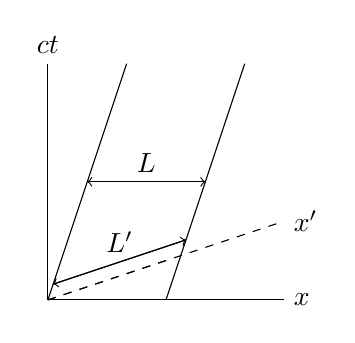
\begin{tikzpicture}
    \draw (0, 0) -- (3, 0) node [right] {$x$};
    \draw (0, 0) -- (0, 3) node [above] {$ct$};
    \draw (0, 0) -- (1, 3);
    \draw (1.5, 0) -- (2.5, 3);
    \draw [->] (0.5, 1.5) -- (2, 1.5) node [pos = 0.5, above] {$L$};
    \draw [->] (2, 1.5) -- (0.5, 1.5);
    \draw [dashed] (0, 0) -- (3, 1) node [right] {$x'$};
    \draw [dashed] (0, 0) -- (1.5, 0.5);
    \draw [->] (0.0667, 0.2) -- (1.75416, 0.7625) node [pos=0.5, above] {$L'$};
    \draw [->] (1.75416, 0.7625) -- (0.0667, 0.2);
  \end{tikzpicture}
\end{center}
The lines $x' = 0$ and $x' = L'$ map into $x = vt$ and $x = vt + L'/\gamma$. So the length in $S$ is $L = L'/\gamma < L'$. Therefore moving objects are contracted in the direction of motion.
\begin{defi}[Proper length]
  The \emph{proper length} is the length measured in an object's rest frame.
\end{defi}

This is analogous to the fact that if you view a bar from an angle, it looks shorter than if you view it from the front. In relativity, what causes the contraction is not a spatial rotation, but a spacetime \emph{hyperbolic} rotation.

Question: does a train of length $2L$ fit alongside a platform of length $L$ if it travels through the station at a speed $v$ such that $\gamma = 2$?

For the system of observers on the platform, the train contracts to a length $2L/\gamma = L$. So it fits.

But for the system of observers on the train, the platform contracts to length $L/\gamma = L/2$, which is much too short!

This can be explained by the difference of lines of simultaneity, since length is the distance between front and back \emph{at the same time}.
\begin{center}
  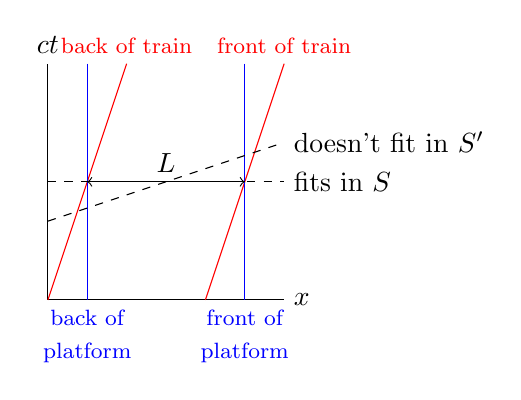
\begin{tikzpicture}
    \draw (0, 0) -- (3, 0) node [right] {$x$};
    \draw (0, 0) -- (0, 3) node [above] {$ct$};
    \draw [red] (0, 0) -- (1, 3) node [above] {\footnotesize back of train};
    \draw [red] (2, 0) -- (3, 3) node [above] {\footnotesize front of train};
    \draw [blue] (0.5, 3) -- (0.5, 0) node [below, align=center] {\footnotesize back of\\\footnotesize platform} ;
    \draw [blue] (2.5, 3) -- (2.5, 0) node [below, align=center] {\footnotesize front of\\\footnotesize platform};
    \draw [->] (0.5, 1.5) -- (2.5, 1.5) node [above, pos=0.5] {$L$};
    \draw [->] (2.5, 1.5) -- (0.5, 1.5);
    \draw [dashed] (0, 1.5) -- (3, 1.5) node [right] {fits in $S$};
    \draw [dashed] (0, 1) -- (3, 2) node [right] {doesn't fit in $S'$};
  \end{tikzpicture}
\end{center}

\subsubsection*{Composition of velocities}
A particle moves with constant velocity $u'$ in frame $S'$, which moves with velocity $v$ relative to $S$. What is its velocity $u$ in $S$?

The world line of the particle in $S'$ is
\[
  x' = u't'.
\]
In $S$, using the inverse Lorentz transformation,
\[
  u = \frac{x}{t} = \frac{\gamma(x' + vt')}{\gamma(t' + (v/c^2) x')} = \frac{u't' + vt'}{t' + (v/c^2)u't'} = \frac{u' + v}{1 + u'v/c^2}.
\]
This is the formula for the relativistic composition of velocities.

The inverse transformation is found by swapping $u$ and $u'$, and swapping the sign of $v$, i.e.
\[
  u' = \frac{u - v}{1 - uv/c^2}.
\]
Note the following:
\begin{itemize}
  \item if $u'v \ll c^2$, then the transformation reduces to the standard Galilean addition of velocities $u \approx u' + v$.
  \item $u$ is a monotonically increasing function of $u$ for any constant $v$ (with $|v| < c$).
  \item When $u' = \pm c$, $u = u'$ for any $v$, i.e.\ the speed of light is constant in all frames of reference.
  \item Hence $|u'| < c$ iff $|u| < c$. This means that we cannot reach the speed of light by composition of velocities.
\end{itemize}

\subsection{Geometry of spacetime}
We'll now look at the geometry of spacetime, and study the properties of vectors in this spacetime. While spacetime has 4 dimensions, and each point can be represented by 4 real numbers, this is not ordinary $\R^4$. This can be seen when changing coordinate systems, instead of rotating the axes like in $\R^4$, we ``squash'' the axes towards the diagonal, which is a \emph{hyperbolic rotation}. In particular, we will have a different notion of a dot product. We say that this space has dimension $d = 1 + 3$.

\subsubsection*{The invariant interval}
In regular Euclidean space, given a vector $\mathbf{x}$, all coordinate systems agree on the length $|\mathbf{x}|$. In Minkowski space, they agree on something else.

Consider events $P$ and $Q$ with coordinates $(ct_1, x_1)$ and $(ct_2, x_2)$ separated by $\Delta t = t_2 - t_1$ and $\Delta x = x_2 - x_1$.

\begin{defi}[Invariant interval]
  The \emph{invariant interval} or \emph{spacetime interval} between $P$ and $Q$ is defined as
  \[
    \Delta s^2 = c^2 \Delta t^2 - \Delta x^2.
  \]
  Note that this quantity $\Delta s^2$ can be both positive or negative --- so $\Delta s$ might be imaginary!
\end{defi}

\begin{prop}
  All inertial observers agree on the value of $\Delta s^2$.
\end{prop}

\begin{proof}
  \begin{align*}
    c^2 \Delta t'^2 - \Delta x'^2 &= c^2 \gamma^2 \left(\Delta t - \frac{v}{c^2}\Delta x\right)^2 - \gamma^2 (\Delta x - v\Delta t)^2\\
    &= \gamma^2 \left(1 - \frac{v^2}{c^2}\right)(c^2 \Delta t^2 - \Delta x^2)\\
    &= c^2\Delta t^2 - \Delta x^2.\qedhere
  \end{align*}
\end{proof}

In three spatial dimensions,
\[
  \Delta s^2 = c^2\Delta t^2 - \Delta x^2 - \Delta y^2 - \Delta z^2.
\]
We take this as the ``distance'' between the two points. For two infinitesimally separated events, we have
\begin{defi}[Line element]
  The \emph{line element} is
  \[
    \d s^2 = c^2 \d t^2 - \d x^2 - \d y^2 - \d z^2.
  \]
\end{defi}

\begin{defi}[Timelike, spacelike and lightlike separation]
  Events with $\Delta s^2 > 0$ are \emph{timelike separated}. It is possible to find inertial frames in which the two events occur in the same position, and are purely separated by time. Timelike-separated events lie within each other's light cones and can influence one another.

  Events with $\Delta s^2 < 0$ are \emph{spacelike separated}. It is possible to find inertial frame in which the two events occur in the same time, and are purely separated by space. Spacelike-separated events lie out of each other's light cones and cannot influence one another.

  Events with $\Delta s^2 = 0$ are \emph{lightlike} or \emph{null separated}. In all inertial frames, the events lie on the boundary of each other's light cones. e.g.\ different points in the trajectory of a photon are lightlike separated, hence the name.
\end{defi}
Note that $\Delta s^2 = 0$ does not imply that $P$ and $Q$ are the same event.

\subsubsection*{The Lorentz group}
The coordinates of an event $P$ in frame $S$ can be written as a \emph{4-vector} (i.e.\ 4-component vector) $X$. We write
\[
  X =
  \begin{pmatrix}
    ct\\
    x\\
    y\\
    z
  \end{pmatrix}
\]
The invariant interval between the origin and $P$ can be written as an inner product
\[
  X\cdot X = X^T\eta X = c^2t^2 - x^2 - y^2 - z^2,
\]
where
\[
  \eta =
  \begin{pmatrix}
    1 & 0 & 0 & 0\\
    0 & -1 & 0 & 0\\
    0 & 0 & -1 & 0\\
    0 & 0 & 0 & -1
  \end{pmatrix}.
\]
4-vectors with $X\cdot X > 0$ are called timelike, and those $X \cdot X < 0$ are spacelike. If $X\cdot X = 0$, it is lightlike or null.

A Lorentz transformation is a linear transformation of the coordinates from one frame $S$ to another $S'$, represented by a $4\times 4$ tensor (``matrix''):
\[
  X' = \Lambda X
\]
Lorentz transformations can be defined as those that leave the inner product invariant:
\[
  (\forall X)(X'\cdot X' = X\cdot X),
\]
which implies the matrix equation
\[
  \Lambda^T\eta \Lambda = \eta.\tag{$*$}
\]
These also preserve $X\cdot Y$ if $X$ and $Y$ are both 4-vectors.

Two classes of solution to this equation are:
\[
  \Lambda =
  \begin{pmatrix}
    1 & 0 & 0 & 0\\
    0\\
    0 & & R\\
    0
  \end{pmatrix},
\]
where $R$ is a $3\times 3$ orthogonal matrix, which rotates (or reflects) space and leaves time intact; and
\[
  \Lambda =
  \begin{pmatrix}
    \gamma & -\gamma \beta & 0 & 0\\
    -\gamma\beta & \gamma & 0 & 0\\
    0 & 0 & 1 & 0\\
    0 & 0 & 0 & 1
  \end{pmatrix},
\]
where $\beta = \frac{v}{c}$, and $\gamma = 1/\sqrt{1 - \beta^2}$. Here we leave the $y$ and $z$ coordinates intact, and apply a Lorentz boost along the $x$ direction.

The set of all matrices satisfying equation $(*)$ form the \emph{Lorentz group} $O(1, 3)$. It is generated by rotations and boosts, as defined above, which includes the absurd spatial reflections and time reversal.

The subgroup with $\det \Lambda = +1$ is the \emph{proper Lorentz group} $SO(1, 3)$.

The subgroup that preserves spatial orientation and the direction of time is the \emph{restricted Lorentz group} $SO^+(1, 3)$. Note that this is different from $SO(1, 3)$, since if you do \emph{both} spatial reflection and time reversal, the determinant of the matrix is still positive. We want to eliminate those as well!

\subsubsection*{Rapidity}
Focus on the upper left $2\times 2$ matrix of Lorentz boosts in the $x$ direction. Write
\[
  \Lambda[\beta] =
  \begin{pmatrix}
    \gamma & -\gamma\beta\\
    -\gamma\beta & \gamma
  \end{pmatrix}
  ,\quad
  \gamma = \frac{1}{\sqrt{1 - \beta^2}}.
\]
Combining two boosts in the $x$ direction, we have
\[
  \Lambda[\beta_1]\Lambda[\beta_2] =
  \begin{pmatrix}
    \gamma_1 & -\gamma_1\beta_1\\
    -\gamma_1\beta_1 & \gamma_1
  \end{pmatrix}
  \begin{pmatrix}
    \gamma_2 & -\gamma_2\beta_2\\
    -\gamma_2\beta_2 & \gamma_2
  \end{pmatrix}
  = \Lambda\left[\frac{\beta_1 + \beta_2}{1 + \beta_1\beta_2}\right]
\]
after some messy algebra. This is just the velocity composition formula as before.

This result does not look nice. This suggests that we might be writing things in the wrong way.

We can compare this with spatial rotation. Recall that
\[
  R(\theta) =
  \begin{pmatrix}
    \cos \theta & \sin \theta\\
    -\sin \theta & \cos \theta
  \end{pmatrix}
\]
with
\[
  R(\theta_1)R(\theta_2) = R(\theta_1 + \theta_2).
\]
For Lorentz boosts, we can define
\begin{defi}[Rapidity]
  The \emph{rapidity} of a Lorentz boot is $\phi$ such that
  \[
    \beta = \tanh \phi,\quad \gamma = \cosh\phi,\quad \gamma\beta=\sinh \phi.
  \]
\end{defi}
Then
\[
  \Lambda[\beta] =
  \begin{pmatrix}
    \cosh \phi & -\sinh \phi\\
    -\sinh \phi & \cosh \phi
  \end{pmatrix}
  = \Lambda(\phi).
\]
The rapidities add like rotation angles:
\[
  \Lambda(\phi_1)\Lambda(\phi_2) = \Lambda(\phi_1 + \phi_2).
\]
This shows the close relation betweens spatial rotations and Lorentz boosts. Lorentz boots are simply \emph{hyperbolic} rotations in spacetime!

\subsection{Relativistic kinematics}
In Newtonian mechanics, we describe a particle by its position $\mathbf{x}(t)$, with its velocity being $\mathbf{u}(t) = \frac{\d \mathbf{x}}{\d t}$.

In relativity, this is unsatisfactory. In special relativity, space and time can be mixed together by Lorentz boosts, and we prefer not to single out time from space. For example, when we write the 4-vector $X$, we put in both the time and space components, and Lorentz transformations are $4\times 4$ matrices that act on $X$.

In the definition of velocity, however, we are differentiating space with respect to time, which is rather weird. First of all, we need something to replace time. Recall that we defined ``proper length'' as the length in the item in its rest frame. Similarly, we can define the \emph{proper time}.

\begin{defi}[Proper time]
  The \emph{proper time} $\tau$ is defined such that
  \[
    \Delta \tau = \frac{\Delta s}{c}
  \]
  $\tau$ is the time experienced by the particle, i.e.\ the time in the particles rest frame.
\end{defi}
The world line of a particle can be parametrized using the proper time by $t(\tau)$ and $\mathbf{x}(\tau)$.
\begin{center}
  \begin{tikzpicture}[yscale=1.3]
    \draw [->] (0, 0) -- (3, 0) node [right] {$x$};
    \draw [->] (0, 0) -- (0, 2.3) node [above] {$ct$};
    \draw (0.7, 0.3) .. controls (0.7, 0.8) and (2, 1.3) .. (2, 1.8);

    \node [circ] at (1.35, 1.05) {};
    \node at (1.35, 1.05) [anchor = north west] {$\tau_1$};
    \node [circ] at (1.93, 1.6) {};
    \node at (1.93, 1.6) [anchor=north west] {$\tau_2$};
  \end{tikzpicture}
\end{center}
Infinitesimal changes are related by
\[
  \d \tau = \frac{\d s}{c} = \frac{1}{c}\sqrt{c^2\;\d t^2 - |\d \mathbf{x}|^2} = \sqrt{1 - \frac{|\mathbf{u}|^2}{c^2}}\;\d t.
\]
Thus
\[
  \frac{\d t}{\d \tau} = \gamma_u
\]
with
\[
  \gamma_u = \frac{1}{\sqrt{1 - \frac{|\mathbf{u}|^2}{c^2}}}.
\]
The total time experienced by the particle along a segment of its world line is
\[
  T = \int \;\d \tau = \int\frac{1}{\gamma_u}\;\d t.
\]
We can then define the \emph{position 4-vector} and \emph{4-velocity}.
\begin{defi}[Position 4-vector and 4-velocty]
  The \emph{position 4-vector} is
  \[
    X(\tau) =
    \begin{pmatrix}
      ct(\tau)\\
      \mathbf{x}(\tau)
    \end{pmatrix}.
  \]
  Its \emph{4-velocity} is defined as
  \[
    U = \frac{\d X}{\d \tau} =
    \begin{pmatrix}
      c\frac{\d t}{\d \tau}\\
      \frac{\d \mathbf{x}}{\d \tau}
    \end{pmatrix}
    = \frac{\d t}{\d \tau}
    \begin{pmatrix}
      c\\
      \mathbf{u}
    \end{pmatrix} = \gamma_u
    \begin{pmatrix}
      c\\
      \mathbf{u}
    \end{pmatrix},
  \]
  where $\mathbf{u} = \frac{\d \mathbf{x}}{\d t}$.
\end{defi}
Another common notation is
\[
  X = (ct, \mathbf{x}),\quad U = \gamma_u (c, \mathbf{u}).
\]
If frames $S$ and $S'$ are related by $X' = \Lambda X$, then the 4-velocity also transforms as $U' = \Lambda U$.

\begin{defi}[4-vector]
  A \emph{4-vector} is a 4-component vectors that transforms in this way under a Lorentz transformation, i.e.\ $X' = \Lambda X$.

  When using suffix notation, the indices are written above (superscript) instead of below (subscript). The indices are written with Greek letters which range from $0$ to $3$. So we have $X^\mu$ instead of $X_i$, for $\mu = 0, 1, 2, 3$. If we write $X_\mu$ instead, it means a different thing. This will be explained more in-depth in the electromagnetism course (and you'll get more confused!).
\end{defi}

$U$ is a 4-vector because $X$ is a 4-vector and $\tau$ is a Lorentz invariant. Note that $\d X/\d t$ is \emph{not} a 4-vector.

Note that this definition of 4-vector is analogous to that of a tensor --- things that transform nicely according to our rules. Then $\tau$ would be a scalar, i.e.\ rank-0 tensor, while $t$ is just a number, not a scalar.

For any 4-vector $U$, the inner product $U\cdot U = U' \cdot U'$ is Lorentz invariant, i.e.\ the same in all inertial frames. In the rest frame of the particle, $U = (c, 0)$. So $U\cdot U = c^2$.

In any other frame, $Y = \gamma_u(c, \mathbf{u})$. So
\[
  Y\cdot Y = \gamma_u^2 (c^2 - |\mathbf{u}|^2) = c^2
\]
as expected.

\subsubsection*{Transformation of velocities revisited}
We have seen that velocities cannot be simply added in relativity. However, the 4-velocity does transform linearly, according to the Lorentz transform:
\[
  U' = \Lambda U.
\]
In frame $S$, consider a particle moving with speed $u$ at an angle $\theta$ to the $x$ axis in the $xy$ plane. This is the most general case for motion not parallel to the Lorentz boost.

Its 4-velocity is
\[
  U =
  \begin{pmatrix}
    \gamma_u c\\
    \gamma_u u\cos \theta\\
    \gamma_u u\sin \theta\\
    0
  \end{pmatrix}, \quad \gamma_u = \frac{1}{\sqrt{1 - u^2/c^2}}.
\]
With frames $S$ and $S'$ in standard configuration (i.e.\ origin coincide at $t = 0$, $S'$ moving in $x$ direction with velocity $v$ relative to $S$),
\[
  U' = \begin{pmatrix}
    \gamma_{u'} c\\
    \gamma_{u'} u'\cos \theta'\\
    \gamma_{u'} u'\sin \theta'\\
    0
  \end{pmatrix}
  =
  \begin{pmatrix}
    \gamma_v & -\gamma_v v/c & 0 & 0\\
    -\gamma_{v} v/c & \gamma_v & 0 & 0\\
    0 & 0 & 1 & 0\\
    0 & 0 & 0 & 1
  \end{pmatrix}
  \begin{pmatrix}
    \gamma_u c\\
    \gamma_u u\cos \theta\\
    \gamma_u u\sin \theta\\
    0
  \end{pmatrix}
\]
Instead of evaluating the whole matrix, we can divide different rows to get useful results.

The ratio of the first two lines gives
\[
  u'\cos \theta' = \frac{u\cos \theta - v}{1 - \frac{uv}{c^2}\cos \theta},
\]
just like the composition of parallel velocities.

The ratio of the third to second line gives
\[
  \tan \theta' = \frac{u\sin \theta}{\gamma_v(u\cos \theta - v)},
\]
which describes \emph{aberration}, a change in the direction of motion of a particle due to the motion of the observer. Note that this isn't just a relativistic effect! If you walk in the rain, you have to hold your umbrella obliquely since the rain seems to you that they are coming from an angle. The relativistic part is the $\gamma_v$ factor in the denominator.

This is also seen in the aberration of starlight ($u = c$) due to the Earth's orbital motion. This causes small annual changes in the apparent positions of stars.
\subsubsection*{4-momentum}
\begin{defi}[4-momentum]
  The \emph{4-momentum} of a particle of mass $m$ is
  \[
    P = mU = m\gamma_u
    \begin{pmatrix}
      c\\
      \mathbf{u}
    \end{pmatrix}
  \]
  The 4-momentum of a system of particles is the sum of the 4-momentum of the particles, and is conserved in the absence of external forces.

  The spatial components of $P$ are the \emph{relativistic 3-momentum},
  \[
    \mathbf{p} = m\gamma_u \mathbf{u},
  \]
  which differs from the Newtonian expression by a factor of $\gamma_u$. Note that $|\mathbf{p}| \to \infty$ as $|\mathbf{u}| \to c$.
\end{defi}

What is the interpretation of the time component $P^0$ (i.e.\ the first time component of the $P$ vector)? We expand for $|\mathbf{u}| \ll c$:
\[
  P^0 = m\gamma c = \frac{mc}{\sqrt{1 - |\mathbf{u}|^2/c^2}} = \frac{1}{c}\left(mc^2 + \frac{1}{2}m|\mathbf{u}|^2 + \cdots\right).
\]
We have a constant term $mc^2$ plus a kinetic energy term $\frac{1}{2}m|\mathbf{u}|^2$, plus more tiny terms, all divided by $c$. So this suggests that $P^0$ is indeed the energy for a particle, and the remaining $\cdots$ terms are relativistic corrections for our old formula $\frac{1}{2}m|\mathbf{u}|^2$ (the $mc^2$ term will be explained later). So we interpret $P$ as
\[
  P =
  \begin{pmatrix}
    E/c\\
    \mathbf{p}
  \end{pmatrix}
\]
\begin{defi}[Relativistic energy]
  The \emph{relativistic energy} of a particle is $E = P^0c$. So
  \[
    E = m\gamma c^2 = mc^2 + \frac{1}{2}m|\mathbf{u}|^2 + \cdots
  \]
\end{defi}
Note that $E\to \infty$ as $|\mathbf{u}| \to c$.

For a stationary particle, we obtain
\[
  E = mc^2.
\]
This implies that mass is a form of energy. $m$ is sometimes called the \emph{rest mass}.

The energy of a moving particle, $m\gamma_u c^2$, is the sum of the rest energy $mc^2$ and kinetic energy $m(\gamma_u - 1)c^2$.

Since $P\cdot P = \frac{E^2}{c^2} - |\mathbf{p}|^2$ is a Lorentz invariant (lengths of 4-vectors are always Lorentz invariant) and equals $m^2 c^2$ in the particle's rest frame, we have the general relation between energy and momentum
\[
  E^2 = |\mathbf{p}|^2 c^2 + m^2c^4
\]
In Newtonian physics, mass and energy are separately conserved. In relativity, mass is not conserved. Instead, it is just another form of energy, and the total energy, including mass energy, is conserved.

Mass can be converged into kinetic energy and vice versa (e.g.\ atomic bombs!)

\subsubsection*{Massless particles}
Particles with zero mass ($m = 0$), e.g.\ photons, can have non-zero momentum and energy because they travel at the speed of light ($\gamma = \infty$).

In this case, $P\cdot P = 0$. So massless particles have light-like (or null) trajectories, and no proper time can be defined for such particles.

Other massless particles in the Standard Model of particle physics include the gluon.

For these particles, energy and momentum are related by
\[
  E^2 = |\mathbf{p}|^2 c^2.
\]
So
\[
  E = |\mathbf{p}|c.
\]
Thus
\[
  P = \frac{E}{c}
  \begin{pmatrix}
    1\\
    \mathbf{n}
  \end{pmatrix},
\]
where $\mathbf{n}$ is a unit (3-)vector in the direction of propagation.

According to quantum mechanics, fundamental ``particles'' aren't really particles but have both particle-like and wave-like properties (if that sounds confusing, yes it is!). Hence we can assign it a \emph{de Broglie wavelength}, according to the \emph{de Broglie relation}:
\[
  |\mathbf{p}| = \frac{h}{\lambda}
\]
where $h \approx \SI{6.63e-34}{\meter\squared\kilogram\per\second}$ is \emph{Planck's constant}.

For massless particles, this is consistent with \emph{Planck's relation}:
\[
  E = \frac{hc}{\lambda} = h\nu,
\]
where $\nu = \frac{c}{\lambda}$ is the \emph{wave frequency}.
\subsubsection*{Newton's second law in special relativity}
\begin{defi}[4-force]
  The \emph{4-force} is
  \[
    F = \frac{\d P}{\d \tau}
  \]
\end{defi}
This equation is the relativistic counterpart to Newton's second law.

It is related to the 3-force $\mathbf{F}$ by
\[
  F = \gamma_u
  \begin{pmatrix}
    \mathbf{F}\cdot \mathbf{u}/c\\
    \mathbf{F}
  \end{pmatrix}
\]
Expanding the definition of the 4-force componentwise, we obtain
\[
  \frac{\d E}{\d \tau} = \gamma_u \mathbf{F}\cdot \mathbf{u} \Rightarrow \frac{\d E}{\d t} = \mathbf{F}\cdot \mathbf{u}
\]
and
\[
  \frac{\d \mathbf{p}}{\d \tau} = \gamma_u \mathbf{F} \Rightarrow \frac{\d \mathbf{p}}{\d t} = \mathbf{F}
\]
Equivalently, for a particle of mass $m$,
\[
  F =mA,
\]
where
\[
  A = \frac{\d U}{\d \tau}
\]
is the 4-acceleration.

We have
\[
  U = \gamma_u
  \begin{pmatrix}
    c\\
    \mathbf{u}
  \end{pmatrix}
\]
So
\[
  A = \gamma_u \frac{\d U}{\d t} = \gamma_u
  \begin{pmatrix}
    \dot{\gamma}_u c\\
    \gamma_u \mathbf{a} + \dot{\gamma}_u \mathbf{u}.
  \end{pmatrix}
\]
where $\mathbf{\mathbf{a}} = \frac{\d \mathbf{u}}{\d t}$ and $\dot{\gamma}_u = \gamma_u^3 \frac{\mathbf{a}\cdot \mathbf{u}}{c^2}$.

In the instantaneous rest frame of a particle, $\mathbf{u} = \mathbf{0}$ and $\gamma_u = 1$. So
\[
  U =
  \begin{pmatrix}
    c\\
    \mathbf{0}
  \end{pmatrix}, \quad
  A =
  \begin{pmatrix}
    0\\
    \mathbf{a}
  \end{pmatrix}
\]
Then $\mathbf{U}\cdot \mathbf{A} = 0$. Since this is a Lorentz invariant, we have $\mathbf{U} \cdot \mathbf{A} = 0$ in all frames.

\subsection{Particle physics}
Many problems can be solved using the conservation of 4-momentum,
\[
  P =
  \begin{pmatrix}
    E/c\\
    \mathbf{p}
  \end{pmatrix},
\]
for a system of particles.
\begin{defi}[Center of momentum frame]
  The \emph{center of momentum (CM) frame}, or \emph{zero momentum frame}, is an inertial frame in which the total 3-momentum is $\sum \mathbf{p} = 0$.
\end{defi}
This exists unless the system consists of one or more massless particle moving in a single direction.

\subsubsection*{Particle decay}
A particle of mass $m_1$ decays into two particles of masses $m_2$ and $m_2$.

We have
\[
  P_1 = P_2 + P_3.
\]
i.e.
\begin{align*}
  E_1 &= E_2 + E_3\\
  \mathbf{p}_1 &= \mathbf{p}_2 + \mathbf{p}_3.
\end{align*}
In the CM frame (i.e.\ the rest frame of the original particle),
\begin{align*}
  E_1 = m_1 c^2 &= \sqrt{|\mathbf{p}_2|^2 c^2 + m_2^2c^4} + \sqrt{|\mathbf{p}_3|^2 c^2 + m_2^2 c^4}\\
  &\geq m_2c^2 + m_3 c^2.
\end{align*}
So decay is possible only if
\[
  m_1 \geq m_2 + m_3.
\]
(Recall that mass is not conserved in relativity!)

\begin{eg}
  A possible decay path of the Higgs' particle can be written as
  \begin{align*}
    \mathrm{h} &\to \gamma \gamma\\
    \text{Higgs'\ particle} &\to 2\text{ photons}
  \end{align*}
  This is possible by the above criterion, because $m_\mathrm{h} \geq 0$, while $m_\gamma = 0$.

  The full conservation equation is
  \[
    P_\mathrm{h} =
    \begin{pmatrix}
      m_\mathrm{h}c\\
      \mathbf{0}
    \end{pmatrix} =
    P_{\gamma_1} + P_{\gamma_2}
  \]
  So
  \begin{align*}
    \mathbf{p}_{\gamma_1} &= \mathbf{p}_{\gamma_2}\\
    E_{\gamma_1} = E_{\gamma_2} &= \frac{1}{2}m_\mathrm{h} c^2.
  \end{align*}
\end{eg}

\subsubsection*{Particle scattering}
When two particles collide and retain heir identities, the total 4-momentum is conserved:
\[
  P_1 + P_2 = P_3 + P_4
\]
In the laboratory frame $S$, suppose that particle 1 travels with speed $u$ and collides with particle 2 (at rest).
\begin{center}
  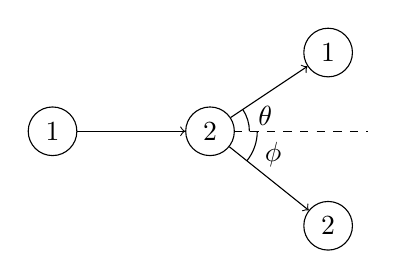
\begin{tikzpicture}
    \node [draw, circle] (1') at (3.5, 1) {1};
    \node [draw, circle] (2') at (3.5, -1.2) {2};
    \node [draw, circle] (2) at (2, 0) {2}
    edge [->] (1')
    edge [->] (2');
    \node [draw, circle] (1) {1}
    edge [->] (2);
    \draw [dashed] (2.3, 0) -- (4, 0);
    \draw (2.5, 0) arc (0:33.69:0.5);
    \draw (2.6, 0) arc (0:-38.66:0.6);
    \node at (2.8, -0.3) {$\phi$};
    \node at (2.7, 0.2) {$\theta$};
  \end{tikzpicture}
\end{center}
In the CM frame $S'$,
\[
  \mathbf{p}'_1 + \mathbf{p}'_2 = 0 = \mathbf{p}_3' + \mathbf{p}'_4.
\]
Both before and after the collision, the two particles have equal and opposite 3-momentum.
\begin{center}
  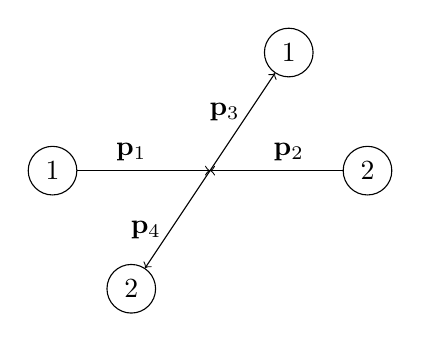
\begin{tikzpicture}
    \node [draw, circle] at (-2, 0) {1}
    edge [->] (0, 0);
    \node [draw, circle] at (2, 0) {2}
    edge [->] (0, 0);
    \node at (-1, 0) [above] {$\mathbf{p}_1$};
    \node at (1, 0) [above] {$\mathbf{p}_2$};
    \node [draw, circle] at (1, 1.5) {1}
    edge [<-] (0, 0);
    \node [draw, circle] at (-1, -1.5) {2}
    edge [<-] (0, 0);
    \node at (0.5, 0.75) [left] {$\mathbf{p}_3$};
    \node at (-0.5, -0.75) [left] {$\mathbf{p}_4$};
  \end{tikzpicture}
\end{center}
The scattering angle $\theta'$ is undetermined and can be thought of as being random. However, we can derive some conclusions about the angles $\theta$ and $\phi$ in the laboratory frame.

(staying in $S'$ for the moment) Suppose the particles have equal mass $m$. They then have the same speed $v$ in $S'$.

Choose axes such that
\[
  P_1' =
  \begin{pmatrix}
    m\gamma_v c\\
    m\gamma_v v\\
    0\\
    0
  \end{pmatrix},\quad
  P_2' =
  \begin{pmatrix}
    m\gamma_v c\\
    -m\gamma_v v\\
    0\\
    0
  \end{pmatrix}
\]
and after the collision,
\[
  P_3' =
  \begin{pmatrix}
    m\gamma_v c\\
    m\gamma_v v\cos \theta'\\
    m\gamma_v v\sin \theta'\\
    0
  \end{pmatrix},\quad
  P_4' =
  \begin{pmatrix}
    m\gamma_v c\\
    -m\gamma_v v\cos \theta'\\
    -m \gamma_v v\sin \theta'\\
    0
  \end{pmatrix}.
\]
We then use the Lorentz transformation to return to the laboratory frame $S$. The relative velocity of the frames is $v$. So the Lorentz transform is
\[
  \Lambda =
  \begin{pmatrix}
    \gamma_v & \gamma_v v/c & 0 & 0\\
    \gamma_v v/c & \gamma_v & 0 & 0\\
    0 & 0 & 1 & 0\\
    0 & 0 & 0 & 1
  \end{pmatrix}
\]
and we find
\[
  P_1 =
  \begin{pmatrix}
    m\gamma_u c\\
    m\gamma_u u\\
    0\\
    0
  \end{pmatrix},\quad
  P_2 =
  \begin{pmatrix}
    mc\\
    0\\
    0\\
    0
  \end{pmatrix}
\]
where
\[
  u = \frac{2v}{1 + v^2/c^2},
\]
(cf.\ velocity composition formula)

Considering the transformations of $P_3'$ and $P_4'$, we obtain
\[
  \tan \theta = \frac{\sin \theta'}{\gamma_v (1 + \cos \theta')} = \frac{1}{\gamma_v}\tan \frac{\theta'}{2},
\]
and
\[
  \tan \phi = \frac{\sin \theta'}{\gamma_v(1 - \cos \theta')} = \frac{1}{\gamma_v}\cot \frac{\theta'}{2}.
\]
Multiplying these expressions together, we obtain
\[
  \tan \theta\tan \phi = \frac{1}{\gamma_v^2}.
\]
So even though we do not know what $\theta$ and $\phi$ might be, they \emph{must} be related by this equation.

In the Newtonian limit, where $|\mathbf{v}| \ll c$, we have $\gamma_v \approx 1$. So
\[
  \tan \theta\tan \phi = 1,
\]
i.e.\ the outgoing trajectories are perpendicular in $S$.

\subsubsection*{Particle creation}
Collide two particles of mass $m$ fast enough, and you create an extra particle of mass $M$.
\[
  P_1 + P_2 = P_3 + P_4 + P_5,
\]
where $P_5$ is the momentum of the new particle.

In the CM frame,
\begin{center}
  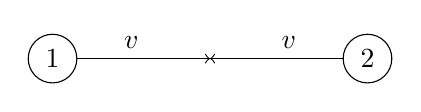
\begin{tikzpicture}
    \node [draw, circle] at (-2, 0) {1}
    edge [->] (0, 0);
    \node [draw, circle] at (2, 0) {2}
    edge [->] (0, 0);
    \node at (-1, 0) [above] {$v$};
    \node at (1, 0) [above] {$v$};
  \end{tikzpicture}
\end{center}
\[
  P_1 + P_2 =
  \begin{pmatrix}
    2m\gamma_v c\\
    \mathbf{0}
  \end{pmatrix}
\]
We have
\[
  P_3 + P_4 + P_5 =
  \begin{pmatrix}
    (E_3 + E_4 + E_5)/c\\
    \mathbf{0}
  \end{pmatrix}
\]
So
\[
  2m\gamma_v c^2 = E_3 + E_4 + E_5 \geq 2mc^2 + Mc^2.
\]
So in order to create this new particle, we must have
\[
  \gamma_v \geq 1 + \frac{M}{2m}.
\]
Alternatively, it occurs only if the initial kinetic energy in the CM frame satisfies
\[
  2(\gamma_v - 1)mc^2 \geq Mc^2.
\]
If we transform to a frame in which the initial speeds are $u$ and 0 (i.e.\ stationary target), then
\[
  u = \frac{2v}{1 + v^2/c^2}
\]
Then
\[
  \gamma_u = 2\gamma_v^2 - 1.
\]
So we require
\[
  \gamma_u \geq 2\left(1 + \frac{M}{2m}\right)^2 - 1 = 1 + \frac{2M}{m} + \frac{M^2}{2m}.
\]
This means that the initial kinetic energy in this frame must be
\[
  m(\gamma_u - 1)c^2 \geq \left(2 + \frac{M}{2m}\right)Mc^2,
\]
which could be much larger than $Mc^2$, especially if $M\gg m$, which usually the case. For example, the mass of the Higgs' boson is 130 times the mass of the proton. So it would be much advantageous to collide two beams of protons head on, as opposed to hitting a fixed target.
\end{document}
